\documentclass[11pt,a4paper]{article}
\usepackage[utf8]{inputenc}
\usepackage[german]{babel}
\usepackage[T1]{fontenc}
\usepackage{amsmath}
\usepackage{amsfonts}
\usepackage{amssymb}
\usepackage{graphicx}
\usepackage[margin=1.25cm]{geometry} % Puts the same margin on all borders of the document

% Packages

\usepackage{hyperref} % Generate hyperlinks to referenced items
\usepackage{adjustbox} % Used to change parameters in \includegraphics[scale=•]{•}
\usepackage{enumitem} % Provides several options for lists
\usepackage{verbatim} % Package to use \begin{comment}
\usepackage{pdfpages} % Used to import PDF pages
\usepackage{multirow} % Allows us to have a single cell in a table span multiple rows
\usepackage{makecell} % Allows us to format multiple lines in a single cell
\usepackage{minted} % Used to syntax highlight code
\usepackage{xcolor}  % Gives access to coloring text
\usepackage{longtable} % Allows us to create a table over multiple pages
\usepackage{float} % Improved placement of floating items
\usepackage{pdfpages} % Used to import pdf pages
\usepackage{booktabs} % Used for horizontal lines instead of \hline



% Settings

\graphicspath{{./files/}} % Sets path for files to the files folder in the same directory

\hypersetup{
    colorlinks=false, %set true if you want colored links
    linktoc=all,     %set to all if you want both sections and subsections linked
    linkcolor=blue,  %choose some color if you want links to stand out
}

\renewcommand{\arraystretch}{1.75} 


\begin{titlepage}
  \title{FOP Reference Sheet} % document_name-type_of_document
  \author{J. Milkovits}
  \date{Last Edited: \today}
\end{titlepage}

\begin{document}

\pagenumbering{gobble}
\maketitle
\pagenumbering{roman} % i, ii, iii on beginning pages, that don't have content
\tableofcontents
\clearpage
\pagenumbering{arabic} % 1,2,3 on content pages

\section{Collections}
	\begin{longtable}{ | p{0.2\textwidth} p{0.75\textwidth} | }
	\hline
	
	\makecell[l]{Informationen } & \makecell[l]{
	$\triangleright$ Sammlungen von Elementen (Objekte eines generischen Typs) \\
	$\triangleright$ Struktur: \\
	\hspace{0.4cm} $\diamond$ Alle Klassen und Interfaces in \texttt{java.util} \\
	\hspace{0.4cm} $\diamond$ Interface \texttt{Collection}: Alle Klassen implementieren dieses Interface \\
	\hspace{0.4cm} $\diamond$ Klasse \texttt{Collections}: Basisalgorithmen, Sortieren \\
	\hspace{0.4cm} $\diamond$ Interface \texttt{List}: Erweitert \texttt{Collection}, mehr Funktionalitäten \\
	\hspace{0.4cm} $\diamond$ Klasse \texttt{Iterator}: Iteration über die Elemente einer \texttt{Collection} \\
	$\triangleright$ Beispiele für Klasse, die das Interface \texttt{Collection} implementieren: \\
	\hspace{0.4cm} $\diamond$ \texttt{Vector, LinkedList, ArrayList, TreeSet, HashSet} } \\ \hline
	
	\makecell[l]{Interface \texttt{Collection}} & \makecell[l]{$\triangleright$ z.B.: \texttt{Collection<Number> c1 = new ArrayList<Number>();} \\
	\hspace{0.4cm} $\diamond$ Speichert leere \texttt{ArrayList} in einer Referenz des Interface \texttt{Collection} \\
	\hspace{0.4cm} $\diamond$ Dies ist möglich, da \texttt{ArrayList} das Interface \texttt{Collection} implementiert \\
	$\triangleright$ Methoden: \\
	\hspace{0.4cm} $\diamond$ \texttt{add}  \\
	\hspace{0.6cm} - Fügt zur ArrayList ein neues Element hinzu \\
	\hspace{0.6cm} - Gibt \texttt{true} zurück, falls Hinzufügen erfolgreich \\
	\hspace{0.4cm} $\diamond$ \texttt{addAll} \\
	\hspace{0.6cm} - Hat eine \texttt{Collection} als Parameter und fügt diese hinzu \\
	\hspace{0.4cm} $\diamond$ \texttt{size} \\
	\hspace{0.6cm} - Anzahl der Elemente als int \\
	\hspace{0.4cm} $\diamond$ \texttt{isEmpty} \\
	\hspace{0.6cm} - \texttt{true}, falls \texttt{Collection} keine Elemente enthält (\texttt{size == 0}) \\ 
	\hspace{0.4cm} $\diamond$ \texttt{contains} \\
	\hspace{0.6cm} - Parameter vom Typ \texttt{Object} \\
	\hspace{0.6cm} - Überprüft, ob aktualer Parameter in \texttt{Collection} vorhanden ist \\
	\hspace{0.6cm} - Nutzt \texttt{equals} von \texttt{Object} $\rightarrow$ Wertgleichheit \\
	\hspace{0.4cm} $\diamond$ \texttt{containsAll} \\
	\hspace{0.6cm} - \texttt{true}, falls ganze übergebene \texttt{Collection} enthalten ist \\
	\hspace{0.4cm} $\diamond$ \texttt{clear} \\
	\hspace{0.6cm} - Entfernt alle Elemente aus der \texttt{Collection} \\
	\hspace{0.4cm} $\diamond$ \texttt{remove} \\
	\hspace{0.6cm} - Entfernt übergebenes \texttt{Object} \\
	\hspace{0.6cm} - \texttt{true}, falls \texttt{Object} mindestens einmal vorhanden \\
	\hspace{0.6cm} - Bei mehreren, entscheidet die \texttt{Collection}-Klasse welches entfernt wird } \\ \hline

	\makecell[l]{Interface \texttt{List}} & \makecell[l]{
	$\triangleright$ Erweitert das Interface \texttt{Collection} \\
	$\triangleright$ Unterschied: Definition einer Reihenfolge auf den Elementen \\
	$\triangleright$ Methoden: \\
	\hspace{0.4cm} $\diamond$ \texttt{indexOf} \\
	\hspace{0.6cm} - Liefert ersten Index zurück, an dem \texttt{Object} zu finden ist \\
	\hspace{0.6cm} - Liefert -1 zurück, falls Parameter nicht in Liste gefunden wird \\
	\hspace{0.4cm} $\diamond$ \texttt{set} \\
	\hspace{0.6cm} - \texttt{T set(int index, T element) ...} \\
	\hspace{0.6cm} - Ersetzt Element an Stelle \texttt{index} durch \texttt{element} \\
	\hspace{0.6cm} - Gibt ersetztes Element zurück \\
	\hspace{0.4cm} $\diamond$ \texttt{add} \\
	\hspace{0.6cm} - Identisch zu Methode \texttt{set}, jedoch ein Unterschied: \\
	\hspace{0.6cm} - Überschreibt das Element \textbf{nicht}, sondern fügt es vor dem Element ein } \\ \hline

	\makecell[l]{Sortieren mit \\ Comparator} & \makecell[l]{
	$\triangleright$ Klasse \texttt{Collections} hat Klassenmethode \texttt{sort} \\
	$\triangleright$ \texttt{Collections.sort(list, new MyComparator());} \\
	\hspace{0.4cm} $\diamond$ Erster Parameter: Zu sortierende Liste (z.B.: \texttt{List<Student> list = ...}) \\
	\hspace{0.4cm} $\diamond$ Zweiter Parameter: Selbst erstellte Sortierlogik \\
	\hspace{0.4cm} $\diamond$ Typparameter von \texttt{Comparator} und \texttt{List} müssen gleich sein } \\ \hline

	\makecell[l]{Interface \texttt{Iterator}} & \makecell[l]{
	$\triangleright$ \texttt{Collection} und \texttt{List} erben von Interface \texttt{Iterable} \\
	$\triangleright$ Jede Klasse, die \texttt{Collection} implementiert hat eine eigene \texttt{Iterator}-Klasse \\
	$\triangleright$ Diese eigene \texttt{Iterator}-Klasse implementiert das Interface \texttt{Iterator} \\
	$\triangleright$ \texttt{Collection<Number> c1 = new ArrayList<Number>();} \\
	$\triangleright$ \texttt{Iterator<Number> it1 = c1.iterator();} \\
	\hspace{0.4cm} $\diamond$ \texttt{Collection} besitzt die Methode \texttt{iterator()} \\
	\hspace{0.4cm} $\diamond$ Liefert ein Objekt ihrer eigenen \texttt{Iterator}-Klasse zurück \\
	$\triangleright$ Methoden: \\
	\hspace{0.4cm} $\diamond$ \texttt{next()} \\
	\hspace{0.6cm} - Liefert ein noch nicht geliefertes Element der \texttt{Collection} \\
	\hspace{0.6cm} - Reihenfolge von Interface abhängig (\texttt{Collection} oder \texttt{List}) \\
	\hspace{0.4cm} $\diamond$ \texttt{hasNext()} \\
	\hspace{0.6cm} - \texttt{true}, falls mindestens ein Element noch nicht durch \\
	\hspace{0.9cm} diesen \texttt{Iterator} zurückgeliefert wurde } \\ \hline

	\makecell[l]{Interface \texttt{Map}} & \makecell[l]{
	$\triangleright$ z.B.: \texttt{Map<String,Integer> map = new HashMap<String,Integer>();} \\
	\hspace{0.4cm} $\diamond$  Erster Typparameter: \texttt{Key} (hier: \texttt{String}) \\
	\hspace{0.4cm} $\diamond$  Typparameter: \texttt{Value} (hier: \texttt{Integer}) \\
	$\triangleright$ Eine \texttt{Map} realisiert eine Abbildung von den \texttt{Keys} in die \texttt{Values} \\
	\hspace{0.4cm} $\diamond$  \texttt{Keys} müssen alle unterschiedlich sein \\
	$\triangleright$ Methoden: \\
	\hspace{0.4cm} $\diamond$ \texttt{put(key, value) // Fügt Paar in Map ein} \\
	\hspace{0.4cm} $\diamond$ \texttt{get(key) // Gibt value zu bestimmtem key zurück} } \\ \hline

	\makecell[l]{\texttt{LinkedList}} & \makecell[l]{
	$\triangleright$ Aufbau: \\
	\hspace{0.4cm} $\diamond$ Elemente der Liste enthalten: \\
	\hspace{0.6cm} - \texttt{Key} vom Typ T \\
	\hspace{0.6cm} - Attribut vom selben Elementtyp mit Namen \texttt{next} \\
	\hspace{0.4cm} $\diamond$ Abspeichern des sogenannten \texttt{head}, dieser speichert die Liste \\
	\hspace{0.4cm} $\diamond$ Die Liste wird durch die Verkettung untereinander mit \texttt{next} erstellt \\
	$\triangleright$ Die folgenden Beispiele sollen nur die Logik hinter der Klasse erläutern \\
	$\triangleright$ Durchlauf durch alle Elemente: (\textbf{LOGIK})\\
	\hspace{0.4cm} $\diamond$ (Die eigentliche Implementation in Java sieht anders aus) \\
	\hspace{0.4cm} $\diamond$ \texttt{for (ListItem<T> p = head; p != null; p = p.next) \{...\}} \\
	\hspace{0.4cm} $\diamond$ Setzen von \texttt{p} zu \texttt{p.next} bis \texttt{p == null} \\
	$\triangleright$ Einfügen Element am Anfang: (\textbf{LOGIK}) \\
	\hspace{0.4cm} $\diamond$ Erstellen eines neuen Listitems und Kopieren der Werte \\
	\hspace{0.4cm} $\diamond$ Achtung: Erst \texttt{head} als \texttt{next} abspeichern \\
	\hspace{0.4cm} $\diamond$ Danach neues Listitem als \texttt{head} setzen \\
	\hspace{0.4cm} $\diamond$ (sonst geht die komplette Liste verloren) \\
	$\triangleright$ Einfügen Element an Stelle n: (\textbf{LOGIK}) \\
	\hspace{0.4cm} $\diamond$ Fortschreiten des Durchlaufs bis zu n-1 \\
	\hspace{0.4cm} $\diamond$ \texttt{ListItem<T> tmp = new ListItem<T>();} \\
	\hspace{0.4cm} $\diamond$ \texttt{tmp.key = key; // Setzen des Keys} \\
	\hspace{0.4cm} $\diamond$ \texttt{tmp.next = p.next; // Knüpfen des neuen Elements an n+1.Element} \\
	\hspace{0.4cm} $\diamond$ \texttt{p.next = tmp; // Knüpfen des n-1.Elements an neues Element} \\
	$\triangleright$ Entfernen Element: (\textbf{LOGIK}) \\ 
	\hspace{0.4cm} $\diamond$ Überspringen des zu löschenden Elements \\
	\hspace{0.4cm} $\diamond$ \texttt{head}: \texttt{head = head.next;} \\
	\hspace{0.4cm} $\diamond$ Sonst: \texttt{p.next = p.next.next;} \\
	\hspace{0.6cm} - Laufpointer muss in diesem Fall eine Stelle davor stehenbleiben \\
	$\triangleright$ Allgemein: \\
	\hspace{0.4cm} $\diamond$ Auf korrektes Zwischenspeichern achten! \\
	$\triangleright$ Doppelte Verkettung: \\
	\hspace{0.4cm} $\diamond$ Ermöglicht rückwarts und vorwärts Durchlaufen \\
	\hspace{0.4cm} $\diamond$ Kostet Laufzeit und Speicher \\
	\hspace{0.4cm} $\diamond$ Verweisnamen meist \texttt{next} und \texttt{backward} \\
	\hspace{0.4cm} $\diamond$ Erhöhter Aufwand, da doppelte Verweiskopien \\
	$\triangleright$ Zyklische Listen: \\
	\hspace{0.4cm} $\diamond$ Letzter Verweis nicht \texttt{null} sondern auf \texttt{head} \\
	} \\ \hline

	\end{longtable}

\section{Computerspeicher}



	\begin{tabular}{ | p{0.2\textwidth} p{0.75\textwidth} | }
	\hline
	\makecell[l]{Unsere Vorstellung} & \makecell[l]{
	$\triangleright$ gro\ss es Feld aus Maschinenwörtern mit eindeutiger Adresse} \\ \hline
	
	\makecell[l]{Erzeugung eines \\ neuen Objekts} & \makecell[l]{
	$\triangleright$ Reservierung von ungenutztem Speicher in ausreichender Grö\ss e} \\ \hline
	
	\makecell[l]{Referenz} & \makecell[l]{
	$\triangleright$ Name der Variable, die die Anfangsadresse des Objekts speichert \\ 
	$\triangleright$ Kann auch an komplett anderer Stelle als das Objekt gespeichert sein } \\ \hline
	
	\makecell[l]{Speicherort primitiver \\ Datentypen} & \makecell[l]{
	$\triangleright$ Name verweist tatsächlich auf Speicherstelle, an der Wert abgespeichet wird } \\ \hline
	
	\makecell[l]{Prozessablauf} & \makecell[l]{
	$\triangleright$ Program Counter enthält Adresse der nächsten Anweisung \\
	\hspace{0.4cm} $\diamond$ Zählt nach jeder Anwendung hoch und verweist auf nächsten Speicher \\
	$\triangleright$ CPU verarbeitet parallel die momentane Anweisung aus Program Counter} \\ \hline
	
	\makecell[l]{Methodenausführung} & \makecell[l]{
	$\triangleright$ Einrichtung einer Variable \texttt{StackPointer} bei Programmstart \\
	$\triangleright$ StackPointer enthält die Adresse des \texttt{Call-Stacks} \\
	$\triangleright$ Bei Methodenaufruf wird im Speicher Platz reserviert, genannt \texttt{Frame} \\
	$\triangleright$ \texttt{Frame}  wird dann auf dem Call-Stack abgelegt\\
	$\triangleright$ Der \texttt{StackPointer}  wird dann mit der Adresse des neuen\texttt{Frames}  überschrieben \\
	$\triangleright$ Methodenaufruf vorbei: Frame wird wieder vom \texttt{Call-Stack} genommen \\
	$\triangleright$ \texttt{StackPointer} wird auf Adresse des vorherigen \texttt{Frames}  gesetzt} \\ \hline
	
	\makecell[l]{Methodentabelle} & \makecell[l]{
	$\triangleright$ Enthält bei Objekt die Anfangsadressen der verfügbaren Methoden } \\ \hline
	
	\end{tabular}
	
	\begin{center}
	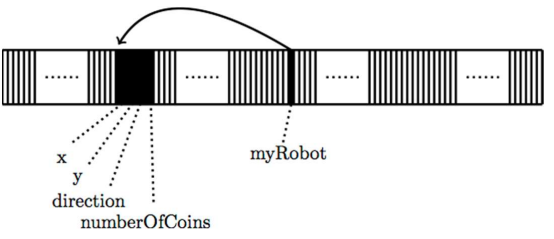
\includegraphics[scale=0.8]{computerspeicher}
	\end{center}

\section{Datenstrukturen}

\begin{tabular}{ | p{0.2\textwidth} p{0.75\textwidth} | }
	\hline
	\makecell[l]{Array} & \makecell[l]{
	$\triangleright$ Verwendet zum Speichern von mehreren Variablen des selben Typs \\
	$\triangleright$ Erzeugung: \texttt{int[] test = new int[n];} \\
	$\triangleright$ \texttt{n} gibt in diesem Fall die feste Anzahl der speicherbaren Variablen an \\
	$\triangleright$ Natürlich auch Arrays von Objekten möglich \\
	$\triangleright$ Zugriff auf Variablen: \texttt{test[0]} für ersten Wert (Index) \\
	$\triangleright$ Zugriff auf Länge: \texttt{test.length} } \\ \hline
	\end{tabular}



\section{Datentypen}

	\begin{tabular}{ | p{0.2\textwidth} p{0.75\textwidth} | }
	\hline

	\makecell[l]{Konstanten} & \makecell[l]{
	$\triangleright$ Variable/Referenz wird dadurch unveränderbar \\
	$\triangleright$ z.B.: \texttt{final myClass ABC = new myClass();} \\
	\hspace{0.4cm} $\diamond$ Referenz zwar nicht veränderbar, Objekt aber schon \\ 
	$\triangleright$ \texttt{Integer.MAX\_VALUE / Integer.MIN\_VALUE} \\
	$\triangleright$ Unendlich: \texttt{Double.POSITIVE\_INFINITY / Double.NEGATIVE\_INFINITY} \\
	$\triangleright$ Müssen initalisiert werden } \\ \hline
	
	\makecell[l]{Primitive Dateitypen} & \makecell[l]{
	$\triangleright$ Ganze Zahlen: byte $\rightarrow$ short $\rightarrow$ int $\rightarrow$ long \\
	$\triangleright$ Gebrochene Zahlen: float $\rightarrow$ double \\
	$\triangleright$ Logik: boolean \\
	$\triangleright$ Zeichen: char \\
	$\triangleright$ Mehrere Definitonen: \texttt{int m = 1, n, k = 2;} \\ 
	$\triangleright$ Ohne Initialisierung: undefinierter Wert} \\ \hline
	
	\makecell[l]{Literale} & \makecell[l]{
	$\triangleright$ wörtlich hingeschriebene Werte eines Datentyps  \\
	$\triangleright$ Zahlen standardmä\ss ig int, falls \texttt{long} gewünscht: \texttt{123L oder 123l} \\ 
	$\triangleright$ Bei gebrochenen double, falls \texttt{float} gewünscht: \texttt{12.3F oder 12.3f} \\
	$\triangleright$ null: Nutzung für Referenzen $\rightarrow$ verweist auf nichts} \\ \hline
	
	\makecell[l]{Boolean} & \makecell[l]{
	$\triangleright$ nur \texttt{true} und \texttt{false} \\
	$\triangleright$ Negation \texttt{!a} \\
	$\triangleright$ Logisches Und: \texttt{a \&\& b} \\
	$\triangleright$ Logisches Oder: \texttt{a || b} (inklusiv) \\
	$\triangleright$ Gleichheit: \texttt{a == b} } \\ \hline
	
	\makecell[l]{Zeichentyp char} & \makecell[l]{
	$\triangleright$ z.B.: \texttt{char c = ´a´;} \\
	$\triangleright$ Interne Kodierung als Unicode \\
	$\triangleright$ \textbackslash t Horizontaler Tab \\
	$\triangleright$ \textbackslash b Backspace \\
	$\triangleright$ \textbackslash n Neue Zeile \\
	$\triangleright$ Auch Darstellung im Hexacode (\textbackslash u039A)} \\ \hline
	
	\makecell[l]{Enumeration} & \makecell[l]{
	$\triangleright$ Zusammenfassung mehrerer Konstanten (feste Anzahl)\\
	$\triangleright$ Erzeugung meist in eigener .java Datei \\
	$\triangleright$ \texttt{enum MyDirection \{DOWN, RIGHT\} } \\
	$\triangleright$ Keine Objekterzeugung von Enumeration möglich \\
	$\triangleright$ Abspeichern in Variable des Enum-Types ist jedoch möglich \\
	$\triangleright$ \texttt{MyDirection dir = MyDirection.DOWN;} \\
	$\triangleright$ Klassenmethoden: \\
	\hspace{0.4cm} $\diamond$ \texttt{values() // Returns array with all enum components} \\
	\hspace{0.4cm} $\diamond$ \texttt{name() // Returns the name of the calling object as string} \\
	 } \\ \hline
	
	\makecell[l]{Referenztypen} & \makecell[l]{
	$\triangleright$ Alle Typen, die keine primitiven Datentypen sind \\
	$\triangleright$ Unterscheidung zwischen Referez und eigentlichem Objekt \\
	$\triangleright$ Gleichheitsoperator \texttt{==} vergleicht nur die Referenz (Objektidentität) \\
	\hspace{0.4cm} $\diamond$ Verweis auf dasselbe Objekt \\
	$\triangleright$ Wertgleichheit bezieht sich auf das Objekt an sich \\
	\hspace{0.4cm} $\diamond$ Deep Copy $\Rightarrow$ An allen parallelen Stellen Wertgleichheit \\
	\hspace{0.4cm} $\diamond$ Shallow Copy $\Rightarrow$ Nur Kopie der Adressen \\
	$\triangleright$ Ohne Initialisierung: Null} \\ \hline
	\end{tabular}


\section{Exceptions (java.lang.Exception;)}

\begin{tabular}{ | p{0.2\textwidth} p{0.75\textwidth} | }
	\hline
	\makecell[l]{Exception-Klassen} & \makecell[l]{
	$\triangleright$ Alle Klassen, die direkt oder indirekt von java.lang.Exception abgeleitet sind} \\ \hline

	\makecell[l]{Exception werfen} & \makecell[l]{
	$\triangleright$ \texttt{throws Exception \{...\}} nach Parameterliste im Methodenkopf \\
	$\triangleright$ Dies signalisiert, dass die Methode mindestens einen Fehler wirft \\
	$\triangleright$ Die geworfene Exception muss vom \texttt{throws}-Typ oder Subtyp sein \\
	$\triangleright$ Auch mehrere Exceptions möglich, mit einem Komma getrennt \\
	$\triangleright$ Werfen der Exception: \\
	\hspace{0.4cm} $\diamond$ z.B.: \texttt{throw new Exception ("No lower case letter!");} \\
	\hspace{0.4cm} $\diamond$ Hier wird als Parameter für die Objekterstellung ein String übergeben \\
	$\triangleright$ \texttt{throws}: \\
	\hspace{0.4cm} $\diamond$ Führt zur Beendung der Methode \\
	\hspace{0.4cm} $\diamond$ Liefert das geworfene Exception-Objekt zurück } \\ \hline

	\makecell[l]{Exception fangen} & \makecell[l]{
	$\triangleright$ Bei Methoden, die Exceptions werfen, wird ein \texttt{try-catch}-Block benötigt \\
	$\triangleright$ Aufbau: \\
	\hspace{0.4cm} $\diamond$ Methoden, die Exceptions werfen in \texttt{try \{...\}} aufrufen \\
	\hspace{0.4cm} $\diamond$ Falls Exception auftritt wird \texttt{catch (Exception exc) \{...\}} aufgerufen \\
	\hspace{0.4cm} $\diamond$ \texttt{catch} muss direkt im Anschluss nach \texttt{try} stehen \\
	\hspace{0.4cm} $\diamond$ Falls kein Fehler auftritt, wird \texttt{catch} übersprungen \\
	\hspace{0.4cm} $\diamond$ Das Programm wird dann normal weiter ausgeführt \\
	$\triangleright$ Es sind auch mehrere \texttt{catch}-Blöcke mit versch. Parametern möglich \\
	$\triangleright$ Methoden: \\
	\hspace{0.4cm} $\diamond$ \texttt{getMessage(); // Returns the error message as a string} \\
	\hspace{0.4cm} $\diamond$ \texttt{printStackTrace(); // Ausgabe des Call-Stacks} \\
	$\triangleright$ Alle möglichen Exceptions müssen durch den \texttt{catch}-Block abgedeckt sein \\
	$\triangleright$ Falls Exception zu mehreren \texttt{catch}-Blöcken 'passt', wird der Erste ausgeführt \\
	\hspace{0.4cm} $\diamond$ Deswegen Reihung der \texttt{catch}-Blöcke von Subtyp nach Supertyp \\
	$\triangleright$ Auch mehrere Exceptions in einem \texttt{catch}-Block möglich mit \texttt{||}} \\ \hline

	\makecell[l]{Weiterreichen} & \makecell[l]{
	$\triangleright$ Weiterreichen der Fehlermeldung durch \texttt{throws} im Methodenkopf möglich \\
	$\triangleright$ Kein \texttt{try-catch}-Block notwendig \\
	$\triangleright$ Main-Methode kann z.B. keine Exceptions weiterreichen} \\ \hline

	\makecell[l]{ \texttt{try-with-ressources} } & \makecell[l]{
	$\triangleright$ Für Ressourcen, die unbedingt wieder geschlossen werden müssen \\
	$\triangleright$ Öffnung der Ressource in runden Klammern: \texttt{try (Printer p =... ) \{...\}} \\
	$\triangleright$ Mehrere Ressourcen möglich, getrennt durch Semikolon } \\ \hline

	\makecell[l]{Runtime Exceptions} & \makecell[l]{
	$\triangleright$ Ausnahme zu \texttt{try}-Blöcken \\
	$\triangleright$ Exceptions von java.lang.RuntimeException und Subtypen \\
	$\triangleright$ z.B.: IndexOutOfBoundsException, NullPointerException \\ 
	$\triangleright$ Grund: Vermeidung von dauerenden \texttt{try}-Blöcken} \\ \hline
	
	\makecell[l]{Throwable und Error} & \makecell[l]{
	$\triangleright$ Exception und Error sind beide von Throwable abgeleitet \\
	$\triangleright$ Alle drei befinden sich im Paket java.lang \\
	$\triangleright$ Error: \\
	\hspace{0.4cm} $\diamond$ Werden geworfen, falls Fehlerbehandlung keinen Sinn macht \\
	\hspace{0.4cm} $\diamond$ Programmabbruch als Ausweg \\
	$\triangleright$ AssertionError: \\
	\hspace{0.4cm} $\diamond$ \texttt{throw new AssertionError("Bad!");} \\
	\hspace{0.4cm} $\diamond$ Kurzform: \texttt{assert x == 2: "Bad!";} \\
	\hspace{0.4cm} $\diamond$ \textbf{Wichtig:} Bedingung muss negiert werden! \\
	\hspace{0.4cm} $\diamond$ Assertanweisungen sinnvoll, da kurz und übersichtlich \\
	\hspace{0.4cm} $\diamond$ Können zusätzlich vom Compiler an- und abgeschaltet werden \\
	\hspace{0.4cm} $\diamond$ z.B.: Verwendung für Tests für Methoden und späteres Abschalten \\
    $\triangleright$ Solche Tests werden White-Box-Tests genannt } \\ \hline
    
    \makecell[l]{Exceptions aus \\ Lambda-Ausdrücken} & \makecell[l]{
    $\triangleright$ Gute Verwendung, falls die funktionale Methode eines Interface Fehler wirft \\
    $\triangleright$ \texttt{MyFuncIntf fct = (m,n) -> } \\
    \hspace{3cm} \texttt{\{if (n == 0) throw new Exception(); return m/n;\};} \\
    $\triangleright$ Funktionale Methode könnte führt Berechnung aus \\
    $\triangleright$ Falls \texttt{n == 0} wird jedoch eine Exception geworfen } \\ \hline

	\end{tabular}

\section{Fehler}
	\begin{tabular}{ | p{0.2\textwidth} p{0.75\textwidth} | }
	\hline

	\makecell[l]{Kompilierzeitfehler \\ (compile-time errors)} & \makecell[l]{
	$\triangleright$ Falsche Klammersetzung, falsche Schlüsselwörter,..\\
	$\triangleright$ Programm wird nicht übersetzt $\Rightarrow$ Fehlermeldung vom Compiler } \\ \hline
	
	\makecell[l]{Laufzeitfehler \\ (run-time errors)} & \makecell[l]{
	$\triangleright$ Tritt während der Ausführung auf \\
	$\triangleright$ Führt zum Abbruch des Programms $\Rightarrow$ Ausgabe der Fehlermeldung \\
	$\triangleright$ Kann nicht vom Compiler entdeckt werden \\
	$\triangleright$ IndexOutOfBounds, NullPointerException,.. } \\ \hline
	\end{tabular}

\section{Files}
	\begin{longtable}{ | p{0.2\textwidth} p{0.75\textwidth} | }
	\hline
	
	\makecell[l]{System Properties \\ (java.lang.System)} & \makecell[l]{
	$\triangleright$ Attribute der Umgebung, in denen das Java Programm abläuft \\
	$\triangleright$ Methoden: \\
	\hspace{0.4cm} $\diamond$ \texttt{getProperty} \\
	\hspace{0.6cm} - Erhält \texttt{String} und gibt \texttt{String} zurück \\ 
	\hspace{0.4cm} $\diamond$ z.B.: \texttt{String homeDir = System.getProperty(\string"user.home\string");} \\
	\hspace{0.4cm} $\diamond$ Mögliche Strings: \\
	\hspace{0.6cm} - \texttt{\string"user.home\string" // Home directory} \\
	\hspace{0.6cm} - \texttt{\string"user.dir\string" // Working directory} \\
	\hspace{0.6cm} - \texttt{\string"user.name\string" // Account name} \\
	\hspace{0.6cm} - \texttt{\string"file.separator\string" // Zeichen zur Dateitrennung} \\
	\hspace{0.6cm} - \texttt{\string"line.separator\string" // Zeichen zur Zeilentrennung} \\
	$\triangleright$ \texttt{System.out}: \\
	\hspace{0.4cm} $\diamond$ Klassenattribut \texttt{out} von System ist von Klasse \texttt{PrintStream} \\
	\hspace{0.4cm} $\diamond$ \texttt{PrintStream} hat also auch Methoden wie \texttt{println} \\
	$\triangleright$ \texttt{System.err}: \\
	\hspace{0.4cm} $\diamond$ Auch \texttt{err} ist von Klasse \texttt{PrintStream} \\
	\hspace{0.4cm} $\diamond$ Hierhin werden die Fehlerausgaben geschrieben \\
	\hspace{0.4cm} $\diamond$ z.B. sinnvoll um Fehler in seperate Log-Datei umzuleiten \\
	$\triangleright$ \texttt{System.in}: \\
	\hspace{0.4cm} $\diamond$ Auch \texttt{in} ist von Klasse \texttt{PrintStream} \\
	\hspace{0.4cm} $\diamond$ Liest Tastatureingaben \\
	$\triangleright$ Diese drei Attribute können auch auf andere Streams gesetzt werden \\
	\hspace{0.4cm} $\diamond$ z.B.: andere \texttt{FileInputStreams/FileOutputStreams} \\
	\hspace{0.4cm} $\diamond$ \texttt{System.setIn(in); System.setOut(out); System.setErr(err);}
	} \\ \hline

	\makecell[l]{Klasse Path / Paths} & \makecell[l]{
	$\triangleright$ Beide in \texttt{java.nio.file} \\
	$\triangleright$ Objekt der Klasse \texttt{Path} verwaltet einen Pfadnamen \\
	\hspace{0.4cm} $\diamond$ Dort muss nicht unbedingt etwas existieren \\
	$\triangleright$ \texttt{Paths} wird nur dazu genutzt um Objekt von \texttt{Path} zu erzeugen \\
	\hspace{0.4cm} $\diamond$ z.B.: \texttt{Path path = Paths.get(homeDir, \string"fop.txt\string");}   } \\ \hline

	\makecell[l]{Klasse Files} & \makecell[l]{
	$\triangleright$ Aus Package \texttt{java.nio.file} \\
	$\triangleright$ Nützliche Sammlung von Klassenmethoden rund um Dateien \\
	$\triangleright$ Methoden: \\
	\hspace{0.4cm} $\diamond$ \texttt{lines // Files.lines(path);} \\
	\hspace{0.6cm} - Öffnet Datei an übergebenem Pfad \\
	\hspace{0.6cm} - Liefert einen Stream von Strings, ein String pro Zeile \\
	\hspace{0.6cm} - Zeilenende durch \texttt{\string"line.separator\string"} gekennzeichnet \\
	\hspace{0.6cm} - \texttt{IOException}, falls Problem beim Öffnen der Datei (\texttt{java.io}) \\
	\hspace{0.4cm} $\diamond$ \texttt{exists // Files.exists(path);} \\
	\hspace{0.6cm} - \texttt{true}, wenn es dort Datei/Verzeichnis gibt \\
	\hspace{0.4cm} $\diamond$ \texttt{isReadable(path)} \\
	\hspace{0.6cm} - Fragt lesende Zugriffsrechte ab \\
	\hspace{0.4cm} $\diamond$ \texttt{isWritable(path)} \\
	\hspace{0.6cm} - Fragt schreibende Zugriffsrechte ab \\
	\hspace{0.4cm} $\diamond$ \texttt{isRegularFile(path)} \\
	\hspace{0.6cm} - \texttt{true}, falls es eine reguläre Datei ist (kein Verzeichnis) \\
	\hspace{0.4cm} $\diamond$ \texttt{isDirectory(path)} \\
	\hspace{0.6cm} - \texttt{true}, falls es ein Verzeichnis ist \\
	\hspace{0.4cm} $\diamond$ \texttt{size(path) // long size = Files.size(path);} \\
	\hspace{0.6cm} - Fragt die Grö\ss e der Datei ab \\
	\hspace{0.6cm} - \texttt{long}, da die Dateigrö\ss e oft nicht in \texttt{int} passt \\
	\hspace{0.4cm} $\diamond$ \texttt{createFile(path)} \\
	\hspace{0.6cm} - Richtet Datei an der übergebenen Stelle ein \\
	\hspace{0.4cm} $\diamond$ \texttt{copy(path1, path2)} \\
	\hspace{0.6cm} - Kopieren von Pfad 1 nach Pfad 2 \\
	\hspace{0.4cm} $\diamond$ \texttt{move(path1, path2)} \\
	\hspace{0.6cm} - Umbenennen einer Datei, oft auch Bewegen genannt \\
	\hspace{0.4cm} $\diamond$ \texttt{delete(path)} \\
	\hspace{0.6cm} - Entfernen einer Datei \\
	\hspace{0.6cm} - \texttt{NoSuchElementException}, falls nicht vorhanden \\
	\hspace{0.4cm} $\diamond$ \texttt{deleteIfExists(path)} \\
	\hspace{0.6cm} - Falls das Objekt nicht existiert, passiert garnichts} \\ \hline
	
	\makecell[l]{Beispiel: \\ Einlesen einer Datei \\  in einen String} & \makecell[l]{
	1 \hspace{0.1cm} \texttt{String homeDir = System.getProperty(\string"user.home\string");} \\
	2 \hspace{0.1cm} \texttt{Path path = Paths.get(homeDir, \string"fop\string", \string"streams.txt\string");} \\
	3 \hspace{0.1cm} \texttt{try (Stream<String> stream = Files.lines(path)) \{ }  \\
	4 \hspace{0.5cm} \texttt{String fileContentAsString = stream.reduce(String::concat);} \\
	5 \hspace{0.1cm} \texttt{\} catch (IOException exc) \{ } \\
	6 \hspace{0.5cm} \texttt{System.out.print(\string"Could not open file\string")} \\
	7 \hspace{0.1cm} \texttt{\}} \\
	$\triangleright$ \texttt{try-with-resources} wird für Interface \texttt{AutoCloseable} verwendet } \\ \hline

	\makecell[l]{Bytedaten} & \makecell[l]{
	$\triangleright$ Direkt, ohne Bezug zu Streams \\
	$\triangleright$ Klassen und Interfaces finden sich in \texttt{java.io} \\
	$\triangleright$ Byteweise Verarbeitung sinnvoll für Audio oder Bilddateien, nicht für Text \\
	$\triangleright$ Wird aber meist durch Bibliotheken oder Ähnliches gehandhabt} \\ \hline

	\makecell[l]{Bytedaten lesen} & \makecell[l]{
	$\triangleright$ Verwendung eines \texttt{InputStream}-Objekts \\
	$\triangleright$ \texttt{InputStream} abstrakt, deswegen nur Subtypen z.B.: \texttt{FileInputStream} \\
	\hspace{0.4cm} $\diamond$ \texttt{FileInputStream} nutzt den Namen der Datei als String im Konstruktor \\
	$\triangleright$ Methoden: \\
	\hspace{0.4cm} $\diamond$ \texttt{read()} \\
	\hspace{0.6cm} - Liest nächstes Byte in ein \texttt{int} \\
	\hspace{0.6cm} - Überprüfung, ob -1 um zu prüfen, ob Dateiende erreicht ist \\
	$\triangleright$ Beispiel: \\
	\hspace{0.4cm} 1 \hspace{0.1cm} \texttt{FileInputStream in = new FileInputStream (fileName);} \\
	\hspace{0.4cm} 2 \hspace{0.1cm} \texttt{int n = in.read();} \\
	\hspace{0.4cm} 3 \hspace{0.1cm} \texttt{if (n == 1) return;} } \\ \hline

	\makecell[l]{Bytedaten schreiben} & \makecell[l]{
	$\triangleright$ Verwendung eines \texttt{OutputStream}-Objekts \\
	$\triangleright$ \texttt{OutputStream} abstrakt, deswegen nur Subtypen z.B.: \texttt{FileOutputStream} \\
	\hspace{0.4cm} $\diamond$ \texttt{FileOutputStream} nutzt den Namen der Datei als String im Konstruktor \\
	\hspace{0.4cm} $\diamond$ Existiert die Datei schon, geht der Inhalt verloren \\
	\hspace{0.4cm} $\diamond$ Existiert die Datei nicht, wird sie erstellt \\
	\hspace{0.4cm} $\diamond$ Zweiter Konstruktor mit \texttt{boolean} als zweiten Paramter: \\
	\hspace{0.6cm} - Falls \texttt{false}: Verhält sich wie normaler Konstruktor \\
	\hspace{0.6cm} - Falls \texttt{true}: Inhalt geht nicht verloren, wird hinten angehangen  \\
	$\triangleright$ Methoden: \\
	\hspace{0.4cm} $\diamond$ \texttt{write()} \\
	\hspace{0.6cm} - Hat \texttt{int} als formalen Parametertyp \\
	\hspace{0.6cm} - Schreibt nur unterestes Byte dieses \texttt{int} \\
	$\triangleright$ Beispiel: \\
	\hspace{0.4cm} 1 \hspace{0.1cm} \texttt{FileOutputStream out = new FileOutputStream(fileName);} \\  
	\hspace{0.4cm} 2 \hspace{0.1cm} \texttt{int i = 5;} \\
	\hspace{0.4cm} 3 \hspace{0.1cm} \texttt{out.write(i);}} \\ \hline

	\makecell[l]{Relevante Subtypen  von \\Input-/OutputStream} & \makecell[l]{
	$\triangleright$ Geschwindigkeit beim Lesen/Schreiben ist relevant \\
	$\triangleright$ \texttt{BufferedInputStream}: \\
	\hspace{0.4cm} $\diamond$ liest mehrere Bytes auf einmal ein \\
	\hspace{0.4cm} $\diamond$ Konstruktor: \texttt{BufferedInputStream(InputStream in)} \\
	\hspace{0.4cm} $\diamond$ Verwendet im Konstruktor z.B. einen \texttt{FileInputStream} \\
	$\triangleright$ \texttt{BufferedOutputStream}: \\
	\hspace{0.4cm} $\diamond$ Schreibt zuerst in internen Puffer \\
	\hspace{0.4cm} $\diamond$ Falls dieser voll ist, wird in die Datei geschrieben \\
	\hspace{0.4cm} $\diamond$ Konstruktor: \texttt{BufferedOutputStream(OutputStream out)} \\
	\hspace{0.4cm} $\diamond$ Schreibt die Daten auf den OutputStream im Parameter \\
	$\triangleright$ \texttt{PrintStream}: \\
	\hspace{0.4cm} $\diamond$ Ersatz für OutputStream im Package \texttt{java.io} \\
	\hspace{0.4cm} $\diamond$ Konstruktor: \texttt{PrintStream(OutputStream out)} \\
	\hspace{0.4cm} $\diamond$ Dient als Konvertierer von primitiven Datentypen und String \\
	\hspace{0.8cm} in die byteweise Darstellung \\
	\hspace{0.4cm} $\diamond$ Das eigentliche Schreiben übernimmt der übergebene \texttt{OutputStream} \\
	\hspace{0.4cm} $\diamond$ Methode \texttt{print} \\ 
	\hspace{0.6cm} - z.B.: \texttt{out1.print(\string"pi = \string"); out1.print(3.14);} \\
	\hspace{0.6cm} - Byteweise Ausgabe von übergebenen Werten \\
	\hspace{0.4cm} $\diamond$ \texttt{System.out.print()}: \texttt{out} ist von Klasse \texttt{PrintStream} \\
	\hspace{0.4cm} $\diamond$ Methode \texttt{println} \\
	\hspace{0.6cm} - Ausgabe von Werten mit Zeilenumbruch} \\ \hline

	\makecell[l]{Mehr Subtypen von \\Input-/OutputStream} & \makecell[l]{
	$\triangleright$ \texttt{java.util.zip.ZipInputStream} \\
	\hspace{0.4cm} $\diamond$ Zum Einlesen von komprimierten Zip-Dateien \\
	$\triangleright$ \texttt{java.util.jar.JarInputStream} \\
	\hspace{0.4cm} $\diamond$ Zum Einlesen von Jar-Dateien \\
	\hspace{0.4cm} $\diamond$ Jar-Dateien enthalten kompilierte Java-Dateien, mit zip komprimiert \\
	$\triangleright$ \texttt{javax.sound.sampled.AudioInputStream} \\
	\hspace{0.4cm} $\diamond$ für Audio-Dateien \\
	$\triangleright$ \texttt{java.io.PipedInputStream / java.io.PipedOutputStream} \\
	\hspace{0.4cm} $\diamond$ Zwei aneinander gekoppelte Lese/Schreib-Klassen
	} \\ \hline

	\makecell[l]{Textdaten direkt} & \makecell[l]{
	$\triangleright$ Bequemere Zugriffsmöglichkeiten für Textdaten vorhanden \\
	$\triangleright$ \texttt{Reader} und \texttt{Writer} aus Package \texttt{java.io} \\
	$\triangleright$ Textdatei besteht aus einzelnen Zeichen aka \texttt{char} \\
	\hspace{0.4cm} $\diamond$ Jedes \texttt{char} ist zwei Byte gro\ss} \\ \hline

	\makecell[l]{Textdaten lesen} & \makecell[l]{
	$\triangleright$ Komplett analog zu \texttt{InputStream} und \texttt{FileInputStream} \\
	$\triangleright$ \texttt{Reader} abstrakt, deswegen nur Subtypen z.B. \texttt{FileReader} \\
	\hspace{0.4cm} $\diamond$ \texttt{FileReader} nutzt den Namen der Datei als String im Konstruktor \\
	$\triangleright$ Methoden: \\
	\hspace{0.4cm} $\diamond$ \texttt{read} \\
	\hspace{0.6cm} - Liest \texttt{char}-Werte ein \\
	\hspace{0.6cm} - Verschiedene Implementationen z.B.: kein Parameter $\rightarrow$ einzelner \texttt{char} \\
	\hspace{0.6cm} - Mit \texttt{char-Array}: Liest soviele ein, bis \texttt{Array} voll ist \\
	$\triangleright$ Beispiel: \\
	\hspace{0.4cm} 1 \hspace{0.1cm} \texttt{FileReader reader1 = new FileReader(fileName);} \\
	\hspace{0.4cm} 2 \hspace{0.1cm} \texttt{char[] buffer = new char[256];} \\
	\hspace{0.4cm} 3 \hspace{0.1cm} \texttt{int n = reader1.read(buffer);} \\
	\hspace{0.4cm} 4 \hspace{0.1cm} \texttt{// n ist in diesem Fall die Anzahl der gelesenen chars} \\
	$\triangleright$ \texttt{BufferedReader} \\
	\hspace{0.4cm} $\diamond$ Konstruktor: \texttt{BufferedReader(Reader in)} \\
	\hspace{0.4cm} $\diamond$ Methode \texttt{readLine();} \\
	\hspace{0.6cm} - Liest alles vom letzten gelesenen Zeichen bis zum Zeilenende \\
	\hspace{0.6cm} - Also meist eine ganze Zeile \\
	$\triangleright$ Verknüpfung mit byteweisem Einlesen: \\
	\hspace{0.4cm} $\diamond$ evtl. sinnvoll, falls offener \texttt{InputStream} auf Text-Datenquelle \\
	\hspace{0.4cm} $\diamond$ Die Brücke bildet hier der Subtyp \texttt{InputStreamReader} \\
	\hspace{0.4cm} 1 \hspace{0.1cm} \texttt{InputStream in = ...;} \\
	\hspace{0.4cm} 2 \hspace{0.1cm} \texttt{Reader reader = new InputStreamReader(in);}} \\ \hline

	\makecell[l]{Textdaten schreiben} & \makecell[l]{
	$\triangleright$ \texttt{Writer} abstrakt, deswegen nur Subtypen z.B. \texttt{FileWriter} \\
	\hspace{0.4cm} $\diamond$ \texttt{FileWriter} benutzt den Namen der Datei als String im Konstruktor \\
	$\triangleright$ Methoden: \\
	\hspace{0.4cm} $\diamond$ \texttt{write} \\
	\hspace{0.6cm} - Schreibt einzelnen \texttt{char} oder ganzen \texttt{String} \\
	$\triangleright$ Beispiel: \\
	\hspace{0.4cm} 1 \hspace{0.1cm} \texttt{FileWriter writer1 = new FileWriter(fileName);} \\
	\hspace{0.4cm} 2 \hspace{0.1cm} \texttt{writer1.write('H');} \\
	\hspace{0.4cm} 3 \hspace{0.1cm} \texttt{writer1.write(\string"ello World\string");} \\ 
	$\triangleright$ Verknüpfung mit byteweisem Schreiben: \\
	\hspace{0.4cm} $\diamond$ Die Brücke bildet hier der Subtyp \texttt{OutputStreamWriter} \\
	\hspace{0.4cm} 1 \hspace{0.1cm} \texttt{OutputStream out = ...;} \\
	\hspace{0.4cm} 2 \hspace{0.1cm} \texttt{Writer writer = new OutputStreamWriter(out);} } \\ \hline

	\end{longtable}

\pagebreak

\section{Functional Interfaces und Lambda-Ausdrücke}

    \begin{longtable}{ | p{0.2\textwidth} p{0.75\textwidth} | } 
    \hline 
    
    \makecell[l]{Functional Interface} & \makecell[l]{
    $\triangleright$ Interface, bei dem genau eine Methode weder \texttt{default} oder \texttt{static} ist \\
    \hspace{0.4cm} $\diamond$ Diese Methode heißt funktionale Methode dieses \texttt{Functional Interface} \\
    $\triangleright$ Jedes \texttt{Functional Interface} hat genau eine funktionale Methode \\
    $\triangleright$ \texttt{Functional Interface} \texttt{IntToDoubleFunction} \\
    \hspace{0.4cm} $\diamond$ Aus Package \texttt{java.util.function} \\
    \hspace{0.4cm} $\diamond$ Hat die funktionale Methode \texttt{double applyAsDouble(int n);}} \\ \hline

    \makecell[l]{Lambda-Ausdrücke \\ Einführung} & \makecell[l]{
    $\triangleright$ Sind Literale von Funktionstypen \\
    $\triangleright$ Abgekürzte Schreibweise für den Aufruf der Hauptmethode eines Func. Interface \\
    $\triangleright$ Verwendung am Beispiel \texttt{IntToDoubleFunction} \textbf{ohne} Lambda: \\
    \hspace{0.6cm} \texttt{IntToDoubleFunction fct1 = new X(2);} \\
    \hspace{0.6cm} \texttt{double y = fct1.applyAsDouble(10);} \\
    \hspace{0.6cm} - \texttt{X} ist hier eine Klasse, die das Interface und die Methode implementiert \\
    $\triangleright$ Verwendung am Beispiel \texttt{IntToDoubleFunction} \textbf{mit} Lambda: \\
    \hspace{0.6cm} \texttt{IntToDoubleFunction fct2 = x -> x * 10;} \\
    \hspace{0.6cm} \texttt{double z = fct2.applyAsDouble(10);} \\
    \hspace{0.6cm} - Richtet nicht sichtbare Klasse ein, die Interface implementiert \\
    \hspace{0.6cm} - Lambda-Ausdruck wird für die funktionale Methode verwendet \\
    \hspace{0.6cm} - Speichern der Referenz eines Objektes dieser Klasse in \texttt{fct2} \\
    } \\ \hline

    \makecell[l]{Closure} & \makecell[l]{
    $\triangleright$ Falls der Parameter (oben 10) zur Laufzeit nicht feststeht (z.B. y): \\
    \hspace{0.4cm} $\diamond$ Unsichtbare Klasse erhält Attribut, das durch Konstruktor initialisiert wird \\
    \hspace{0.4cm} $\diamond$ Verwendung dieses Attributs innerhalb der Klasse \\
    $\triangleright$ Info aus Entstehungskontext des Lambda-Ausdrucks wird mitgespeichert \\
    \hspace{0.4cm} $\diamond$ Aktualer Wert aber nicht unbedingt kopiert, sondern referenziert \\
    \hspace{0.4cm} $\diamond$ Vorsicht bei Änderungen  } \\ \hline

    \makecell[l]{Lambda-Ausdrücke \\ Aufbau} & \makecell[l]{
    $\triangleright$ \texttt{n -> n \SI{}{\percent} 2 == 1} \\
    \hspace{0.4cm} $\diamond$ Kurzform  \\
    $\triangleright$ \texttt{(int n) ->\{return n \SI{}{\percent} 2 == 1;\}} \\
    \hspace{0.4cm} $\diamond$ richtige lange Form, Typangabe des Parameters optional \\
    $\triangleright$ \texttt{(int n, double x) -> \{System.out.print(x); System.out.print(n);\}} \\
    \hspace{0.4cm} $\diamond$ Langform ermöglicht mehrere Anweisungen } \\ \hline

    \makecell[l]{Beispiel Prädikate} & \makecell[l]{
    $\triangleright$ Prädikat: boolsche Funktione, die entweder \texttt{true} oder \texttt{false} zurückliefert \\
    $\triangleright$ Gut für Methoden, die z.B. variablen Filter implementieren \\
    $\triangleright$ \texttt{java.util.function.IntPredicate}: \\
    \hspace{0.4cm} $\diamond$ Funktionale Methode \texttt{boolean test(int x);} \\
    \hspace{0.4cm} $\diamond$ Beispiel: \\
    \hspace{0.6cm} - \texttt{IntPredicate pred1 = n -> n \SI{}{\percent} 2 == 1} \\
    \hspace{0.6cm} - Gibt \texttt{true} zurück, falls \texttt{n} ungerade ist \\
    $\triangleright$ \texttt{java.util.function.IntPredicate} hat noch \texttt{default}-Methoden: \\
    \hspace{0.4cm} $\diamond$ Zugriff auf diese über \texttt{pred1}: \\
    \hspace{0.6cm} - \texttt{IntPredicate pred4 = pred1.negate();} \\
    \hspace{0.6cm} - Die Klasse des Objekts \texttt{pred1} implementiert ja das Interface \\
    \hspace{0.4cm} $\diamond$ Ergänzung des \texttt{Functional Interface} durch diese \texttt{default}-Methoden  \\
    $\triangleright$ Natürlich auch Array-Erstellung eines Interface möglich \\
    \hspace{0.4cm} $\diamond$ \texttt{IntPredicate[] predicates = new IntPredicate[6];} \\
    \hspace{0.4cm} $\diamond$ \texttt{predicates[0] = n -> n > 0;} \\
    $\triangleright$ Auch Erstellung einer Liste möglich \\
    \hspace{0.4cm} $\diamond$ \texttt{List<IntPredicate> pred = new ArrayList<IntPredicate>();} \\
    \hspace{0.4cm} $\diamond$ \texttt{pred.add(n -> n > 0);} } \\ \hline

    \makecell[l]{Methodennamen \\ als Lambda} & \makecell[l]{
    $\triangleright$ Für Lambda-Ausdrücke, die nur aus einzelnem Methodenaufruf bestehen \\
    \hspace{0.4cm} $\diamond$ Fachbegriff \texttt{method reference} \\
    $\triangleright$ Normalerweise: \texttt{... = x -> \{System.out.print(x);\}} \\
    $\triangleright$ Hier: \texttt{... = System.out::print;} \\
    \hspace{0.4cm} $\diamond$ Verbinden des Methodennamens mit Referenz auf Objekt durch Doppelpunkt \\
    \hspace{0.4cm} $\diamond$ Funktioniert auch analog mit Klassenmethoden} \\ \hline

    \end{longtable}

\section{Graphical User Interface}
	\begin{longtable}{ | p{0.2\textwidth} p{0.75\textwidth} | }
	\hline
	
	\makecell[l]{Window Manager} & \makecell[l]{
	$\triangleright$ Systemprozess, der permanent im Hintergrund als \texttt{Service} läuft \\
	$\triangleright$ Stellt generelle, anwendungsunspezifische Funktionalitäten zur Verfügung \\
	\hspace{0.4cm} $\diamond$ Öffnen, Schlie\ss en, Ikonifizieren, Grö\ss e ändern \\
	\hspace{0.4cm} $\diamond$ Rahmen um Fenster, Bildschirmhintergrund } \\ \hline

	\makecell[l]{Klasse Frame} & \makecell[l]{
	$\triangleright$ Abgeleitet von \texttt{java.awt.Window;} (awt = abstract window toolkit) \\
	$\triangleright$ Im Gegensatz zu \texttt{Window} aber mit Rahmen (vom \texttt{Window Manager} verwaltet) \\
	$\triangleright$ Beispielkonstruktor: \texttt{Frame frame = new Frame(string); // Fenstertitel} \\
	$\triangleright$ Vorhergehensweise: \\
	\hspace{0.4cm} $\diamond$ Erstellung einer Klasse, die \texttt{Frame} erweitert \\
	\hspace{0.4cm} $\diamond$ Hinzufügen von Funktionalitäten \\
	$\triangleright$ Methoden: \\
	\hspace{0.4cm} $\diamond$ \texttt{setVisible(boolean b)} \\ 
	\hspace{0.6cm} - \texttt{Frame} ist entweder sichtbar oder unsichtbar \\ 
	\hspace{0.6cm} - Standardmä\ss ig unsichtbar \\
	\hspace{0.6cm} - Erst Fenster aufbauen, dann sichtbar machen \\
	\hspace{0.4cm} $\diamond$ \texttt{setBackground(Color bgColor)} \\
	\hspace{0.6cm} - Setzt die Hintergrundfarbe des Fensters \\
	\hspace{0.4cm} $\diamond$ \texttt{dispose()} \\
	\hspace{0.6cm} - Alle Ressourcen des Fensters und der Bestandteile werden freigegeben \\
	\hspace{0.4cm} $\diamond$ \texttt{setExtendedState(int state)} \\
	\hspace{0.6cm} - Setzt den Status des Fensters \\
	\hspace{0.6cm} - \texttt{ICONIFIED}: Ikonifiziert das Fenster \\
	\hspace{0.6cm} - \texttt{NORMAL}: Deikonifiziert das Fenster \\
	\hspace{0.6cm} - \texttt{MAXIMIZED\_HORIZ}: Ausbreitung auf gesamte Horizontale \\
	\hspace{0.4cm} $\diamond$ \texttt{add(Component comp)} \\
	\hspace{0.6cm} - Fügt den übergebenen Komponenten zum \texttt{Frame} hinzu \\
	} \\ \hline

	\makecell[l]{Komponenten} & \makecell[l]{
	$\triangleright$ Eigene Klasse für jede Komponente \\
	$\triangleright$ Alle Klassen oder Interfaces aus \texttt{java.awt}, falls nicht anders gesagt \\
	$\triangleright$ Werden mithilfe von \texttt{add(Component comp)} zum Fenster hinzugefügt } \\ \hline

	\makecell[l]{Button} & \makecell[l]{$\triangleright$ Konstruktor: \texttt{Button(String label) // Text auf dem Button} \\
	$\triangleright$ Methoden: \\
	\hspace{0.4cm} $\diamond$ \texttt{setFont(Font f)} \\
	\hspace{0.6cm} - Zum Setzen der Schriftart \\
	\hspace{0.6cm} - Konstruktor \texttt{Font: Font(String name, int style, int size)} \\
	\hspace{0.4cm} $\diamond$ \texttt{addActionListener(ActionListener l)} \\
	\hspace{0.6cm} - Fügt den übergebenen \texttt{ActionListener} hinzu \\ 
	\hspace{0.6cm} - Bei jedem Klick wird \texttt{actionPerformed} des \texttt{Listeners} aufgerufen \\
	\hspace{0.6cm} - Auch mehrere möglich \\
    \hspace{0.6cm} - Automatische Einrichtung des \texttt{Event Dispatch Thread} \\
	\hspace{0.4cm} $\diamond$ \texttt{setLabel(String label)} \\
	\hspace{0.6cm} - Setzt den Titel des \texttt{Button}
	} \\ \hline

	\makecell[l]{Interface \\ ActionListener} & \makecell[l]{
	$\triangleright$ Zugehörig zu \texttt{Button} \\
	$\triangleright$ Aus Package \texttt{java.awt.event} \\
	$\triangleright$ Funktionales Interface \\
	$\triangleright$ Funktionale Methode \texttt{actionPerformed (ActionEvent event)} \\
	$\triangleright$ Vorhergehensweise: \\
	\hspace{0.4cm} $\diamond$ Erstellen einer eigenen Klasse, die \texttt{ActionListener} implementiert \\
	\hspace{0.4cm} $\diamond$ Erstellen relevanter Attribute und Konstruktor für gegebenen Fall \\
	\hspace{0.4cm} $\diamond$ Implemetieren der Methode \texttt{actionPerformed (ActionEvent event)} \\
	\hspace{0.4cm} $\diamond$ Erstellen eines Objekts unserer Klasse \\ 
	\hspace{0.6cm} - \texttt{ActionListener listener = new MyListener(frame);} \\
	\hspace{0.4cm} $\diamond$ Hinzufügen des \texttt{Listener} zum \texttt{Button} \\
	\hspace{0.6cm} - \texttt{button.addActionListener(listener);} \\
	$\triangleright$ Alternativ: \\
	\hspace{0.4cm} $\diamond$ Erstellung des \texttt{Listener} in der Subklasse des \texttt{Frame} \\ 
	\hspace{0.6cm} - Keine \texttt{Frame}-Übergabe notwendig \\
    \hspace{0.6cm} - z.B.: als \texttt{private}-Klasse (Stichwort: \texttt{nested classes}) \\
    $\triangleright$ Da \texttt{Functional Interface}: Lambda-Ausdruck \\
    \hspace{0.4cm} $\diamond$ \texttt{button.addActionListener( (e) -> \{System.out.print("Hello");\})}
	 } \\ \hline

	\makecell[l]{Klasse ActionEvent} & \makecell[l]{
	$\triangleright$ Übergebener Parameter bei \texttt{actionPerformed} \\
	$\triangleright$ Methoden: \\
	\hspace{0.4cm} $\diamond$ \texttt{getWhen()} \\
	\hspace{0.6cm} - Gibt die Uhrzeit des Geschehnisses als \texttt{long} zurück \\
	\hspace{0.6cm} - Nützlich: \texttt{java.sql.Timestamp} \\
	\hspace{0.6cm} - \texttt{Timestamp stamp = new Timestamp (event.getWhen());} \\ 
	\hspace{0.6cm} - Methoden: \texttt{stamp.getHour(); stamp.getMinute();}} \\ \hline

	\makecell[l]{Übersicht Listener \\ und Events} & \makecell[l]{
	$\triangleright$ \texttt{Listener}-Interface $\leftrightarrow$ \texttt{Event}-Klasse \\
	$\triangleright$ \texttt{KeyListener} $\leftrightarrow$ \texttt{KeyEvent} \\
	$\triangleright$ \texttt{MouseListener} $\leftrightarrow$ \texttt{MouseEvent} \\
	$\triangleright$ \texttt{MouseMotionListener} $\leftrightarrow$ \texttt{MouseEvent} \\
	$\triangleright$ \texttt{MouseWheelListener} $\leftrightarrow$ \texttt{MouseWheelEvent} \\ 
	$\triangleright$ \texttt{WindowFocusListener} $\leftrightarrow$ \texttt{WindowEvent} \\
	$\triangleright$ \texttt{WindowListener} $\leftrightarrow$ \texttt{WindowEvent} \\ 
	$\triangleright$ \texttt{WindowStateListener} $\leftrightarrow$ \texttt{WindowEvent} \\
	$\triangleright$ Hinzufügen: \\
	\hspace{0.4cm} $\diamond$ \texttt{addKeyListener(...)} \\
	\hspace{0.4cm} $\diamond$ \texttt{addMouseListener(...)} \\
	\hspace{0.4cm} $\diamond$ \texttt{addWindowListener(...)} } \\ \hline

	\makecell[l]{Adapter} & \makecell[l]{
	$\triangleright$ Verwendung von Adaptern, wenn passendes Interface nicht \texttt{functional} ist \\
	\hspace{0.4cm} $\diamond$ z.B. Interface \texttt{KeyListener, MouseListener,..} \\
	\hspace{0.4cm} $\diamond$ Diese Interfaces besitzen mehrere Methoden \\
	$\triangleright$ Adapter sind Klassen und bestehen zu jedem \texttt{Listener}-Interface \\
	\hspace{0.4cm} $\diamond$ z.B.: \texttt{KeyAdapter, MouseAdapter} \\
	\hspace{0.4cm} $\diamond$ Diese Adapter implementieren das dazugehörige Interface \\
	\hspace{0.4cm} $\diamond$ Die Methoden werden jedoch leer gelassen \\
	$\triangleright$ Vorteil vom Adapter: \\
	\hspace{0.4cm} $\diamond$ Nicht alle Methoden müssen implementiert werden \\
	\hspace{0.4cm} $\diamond$ Nur die genutzten Methoden (z.B.: \texttt{keyPressed()}) werden implementiert \\
	$\triangleright$ Verwendung: \\
	\hspace{0.4cm} $\diamond$ Erweitern der eigenen \texttt{Listener}-Klasse mit Adapter \\
	\hspace{0.4cm} $\diamond$ z.B.: \texttt{public class MyKeyListener extends KeyAdapter \{...\}}} \\ \hline

	\makecell[l]{Interface KeyListener} & \makecell[l]{
	$\triangleright$ Abhorchen der Tastatur \\
	$\triangleright$ Erstellen eigener Klasse, die die Klasse \texttt{KeyAdapter} (siehe Adapter) erweitert \\
	$\triangleright$ Methoden: \\
	\hspace{0.4cm} $\diamond$ \texttt{public void keyPressed (KeyEvent event)} \\
	\hspace{0.6cm} - Wird beim Herunterdrücken einer Taste ausgeführt \\
	\hspace{0.4cm} $\diamond$ \texttt{public void keyReleased (KeyEvent event)} \\
	\hspace{0.6cm} - Wird beim Loslassen einer Taste ausgeführt \\
	\hspace{0.4cm} $\diamond$ \texttt{public void keyTyped (KeyEvent event)} \\
	\hspace{0.6cm} - Wird beim Antippen einer Taste ausgeführt} \\ \hline

	\makecell[l]{Klasse KeyEvent} & \makecell[l]{
	$\triangleright$ Übergebener Parameter bei z.B.: \texttt{keyPressed} \\
	$\triangleright$ Methoden: \\
	\hspace{0.4cm} $\diamond$ \texttt{getKeyCode()} \\
	\hspace{0.6cm} - Liefert die Kodierung der gedrückten Taste zurück \\
	$\triangleright$ Klassenkonstanten für jede Taste: \\
	\hspace{0.4cm} $\diamond$ z.B.: \texttt{KeyEvent.VK\_A // Buchstabe A} \\
	\hspace{0.4cm} $\diamond$ z.B.: \texttt{KeyEvent.VK\_COLON // Doppelpunkt} \\
	\hspace{0.4cm} $\diamond$ z.B.: \texttt{KeyEvent.VK\_BACKSPACE // Backspace Taste} \\
	$\triangleright$ Beispiel Verwendung: \\
	\hspace{0.4cm} 1 \hspace{0.1cm} \texttt{public class MyKeyListener extends KeyAdapter \{} \\
	\hspace{0.4cm} 2 \hspace{0.5cm} \texttt{public void keyPressed (KeyEvent event) \{} \\
	\hspace{0.4cm} 3 \hspace{0.9cm} \texttt{switch (event.getKeyCode()) \{}	\\
	\hspace{0.4cm} 4 \hspace{1.3cm} \texttt{case KeyEvent.VK\_A: ... break;} \\
	\hspace{0.4cm} 5 \hspace{1.3cm} \texttt{case KeyEvent.VK\_COLON: ... break;} \\
	\hspace{0.4cm} 6 \hspace{1.3cm} \texttt{case KeyEvent.VK\_Backspace: ... break;} \\
	\hspace{0.4cm} 7 \hspace{0.9cm} \texttt{\}} \\
	\hspace{0.4cm} 8 \hspace{0.5cm} \texttt{\}} \\
	\hspace{0.4cm} 9 \hspace{0.1cm} \texttt{\}}
	} \\ \hline

	\makecell[l]{Interface \\ MouseListener} & \makecell[l]{
	$\triangleright$ Abhorchen der Maus \\
	$\triangleright$ Erstellen eigener Klasse, die die Klasse \texttt{MouseAdapter} erweitert \\
	\hspace{0.4cm} $\diamond$ \texttt{MouseAdapter} implementiert alle drei \texttt{Mouse}-Interfaces \\
	\hspace{0.4cm} $\diamond$  \texttt{MouseListener, MouseMotionListener, MouseWheelListener} \\
	$\triangleright$ Methoden: \\
	\hspace{0.4cm} $\diamond$ \texttt{public void mouseClicked (MouseEvent event)} \\
	\hspace{0.6cm} - Wird beim kurzen Klicken der Maustaste ausgeführt \\
	\hspace{0.4cm} $\diamond$ \texttt{public void mousePressed (MouseEvent event)} \\	
	\hspace{0.6cm} - Wird beim Herunterdrücken der Maustaste ausgeführt \\
	\hspace{0.4cm} $\diamond$ \texttt{public void mouseReleased (MouseEvent event)} \\
	\hspace{0.6cm} - Wird beim Loslassen der Maustaste ausgeführt \\
	\hspace{0.4cm} $\diamond$ \texttt{public void mouseEntered (MouseEvent event)} \\
	\hspace{0.6cm} - Wird ausgeführt, sobald der Mauszeiger den abgehorchten Bereich betritt \\
	\hspace{0.4cm} $\diamond$ \texttt{public void mouseExited (MouseEvent event)} \\
	\hspace{0.6cm} - Wird ausgeführt, sobald der Mauszeiger den abgehorchten Bereich verlässt} \\ \hline

	\makecell[l]{Interface \\ MouseMotionListener} & \makecell[l]{
	$\triangleright$ Abhorchen der Mausbewegung \\
	$\triangleright$ Methoden sind auch in Klasse \texttt{MouseAdapter} enthalten \\
	$\triangleright$ Methoden: \\
	\hspace{0.4cm} $\diamond$ \texttt{public void mouseDragged (MouseEvent event)} \\
	\hspace{0.4cm} $\diamond$ \texttt{public void mouseMoved (MouseEvent event)}  } \\ \hline

	\makecell[l]{Interface \\ MouseWheelListener} & \makecell[l]{
	$\triangleright$ Abhorchen der Mausradbewegung \\
	$\triangleright$ Methoden sind auch in Klasse \texttt{MouseAdapter} enthalten \\
	$\triangleright$ Methoden: \\
	\hspace{0.4cm} $\diamond$ \texttt{public void mouseWheelMoved (MouseWheelEvent event)}} \\ \hline

	\makecell[l]{Klasse MouseEvent} & \makecell[l]{
	$\triangleright$ Übergebener Parameter bei z.B.: \texttt{mouseClicked} \\
	$\triangleright$ Methoden: \\
	\hspace{0.4cm} $\diamond$ \texttt{getButton()} \\
	\hspace{0.6cm} - Liefert die gedrückte Taste zurück \\
	\hspace{0.4cm} $\diamond$ \texttt{getX()} \\
	\hspace{0.6cm} - Liefert x-Koordinate abhängig vom Ursprung des Bereichs \\
	\hspace{0.4cm} $\diamond$ \texttt{getY()} \\
	\hspace{0.6cm} - Liefert y-Koordinate abhängig vom Ursprung des Bereichs \\
	$\triangleright$ Klassenkonstanten für Maustasten: \\
	\hspace{0.4cm} $\diamond$ \texttt{MouseEvent.BUTTON1} \\
	\hspace{0.4cm} $\diamond$ \texttt{MouseEvent.BUTTON2}} \\ \hline

	\makecell[l]{Klasse \\ MouseWheelEvent} & \makecell[l]{
	$\triangleright$ Übergebener Parameter bei z.B.: \texttt{mouseWheelMoved} \\
	$\triangleright$ Methoden: \\
	\hspace{0.4cm} $\diamond$ \texttt{getWheelRotation()} \\
	\hspace{0.6cm} - Liefert die Anzahl der gedrehten "Ticks"  } \\ \hline

	\makecell[l]{Interface \\ WindowListener} & \makecell[l]{
	$\triangleright$ Abhorchen von Fensteraktionen \\
	$\triangleright$ Erstellen eigener Klasse, die die Klasse \texttt{WindowAdapter} erweitert \\
	\hspace{0.4cm} $\diamond$ \texttt{WindowAdapter} implementiert alle drei \texttt{Window}-Interfaces \\
	\hspace{0.4cm} $\diamond$ \texttt{WindowListener, WindowStateListener, WindowFocusListener} \\
	$\triangleright$ Methoden: \\
	\hspace{0.4cm} $\diamond$ \texttt{public void windowOpened (WindowEvent event)} \\
	\hspace{0.4cm} $\diamond$ \texttt{public void windowClosing (WindowEvent event)} \\
	\hspace{0.4cm} $\diamond$ \texttt{public void windowClosed (WindowEvent event)} \\
	\hspace{0.4cm} $\diamond$ \texttt{public void windowClosed (WindowEvent event)} \\
	\hspace{0.4cm} $\diamond$ \texttt{public void windowDeactivated (WindowEvent event)} \\
	\hspace{0.4cm} $\diamond$ \texttt{public void windowIconified (WindowEvent event)} \\
	\hspace{0.4cm} $\diamond$ \texttt{public void windowDeiconified (WindowEvent event)}} \\ \hline

	\makecell[l]{Interface \\ WindowStateListener} & \makecell[l]{
	$\triangleright$ Abhorchen des Status des Fensters \\
	$\triangleright$ Methoden sind auch in \texttt{WindowAdapter} vorhanden \\
	$\triangleright$ Methoden: \\
	\hspace{0.4cm} $\diamond$ \texttt{public void windowStateChanged ( WindowEvent event )}} \\ \hline

	\makecell[l]{Interface \\ WindowFocusListener} & \makecell[l]{
	$\triangleright$ Abhorchen des Fokus im Bezug auf das Fenster \\
	$\triangleright$ Methoden sind auch in \texttt{WindowAdapter} vorhanden \\
	$\triangleright$ Methoden: \\
	\hspace{0.4cm} $\diamond$ \texttt{public void windowGainedFocus ( WindowEvent event )} \\
	\hspace{0.4cm} $\diamond$ \texttt{public void windowLostFocus ( WindowEvent event )} } \\ \hline

	\makecell[l]{Klasse Canvas} & \makecell[l]{
	$\triangleright$ abgegrenzte Zeichenfläche in einem Fenster \\
	$\triangleright$ Vorhergehensweise: \\
	\hspace{0.4cm} $\diamond$ Erstellung eigener Subtyp-Klasse von \texttt{Canvas} \\
	\hspace{0.4cm} $\diamond$ Implementieren der Methode \texttt{public void paint (Graphics graphics)} \\
	\hspace{0.4cm} $\diamond$ Füllen der Methode mit eigener Zeichenlogik \\
	\hspace{0.4cm} $\diamond$ Verwendung von \texttt{java.awt.Graphics;} \\
	\hspace{0.4cm} $\diamond$ Hinzufügen zum \texttt{Frame} mithilfe von \texttt{add} \\
	$\triangleright$ Beleuchtung nützlicher Aspekte von Graphics: \\
	$\triangleright$ \texttt{FontMetrics} \\
	\hspace{0.4cm} $\diamond$ Informationen über festgelegte Schriftart und Schriftgrö\ss e \\
	\hspace{0.4cm} $\diamond$ Abfrage: \\
	\hspace{0.6cm} - \texttt{FontMetrics fontM = graphics.getFontMetrics();} \\
	\hspace{0.4cm} $\diamond$ Abfrage der maximalen Stringhöhe: \\
	\hspace{0.6cm} - \texttt{int maxHeight = fontM.getMaxAscent() + fontM.getMaxDescent();} \\
	\hspace{0.6cm} - Methoden geben maximalen Abstand von der Basislinie des Textes an \\
	\hspace{0.4cm} $\diamond$ Abfrage der Stringbreite von gegebenem String: \\
	\hspace{0.6cm} - \texttt{int widthStr = fontMetrics.stringWidth(string);} \\
	$\triangleright$ Abfrage des Zeichenfensters als Rechteck: \\
	\hspace{0.6cm} - \texttt{Rectangle area = graphics.getClipBounds();} \\
	\hspace{0.6cm} - \texttt{x} und \texttt{y} geben den Ursprung an \\
	\hspace{0.6cm} - \texttt{width} und \texttt{height} die Breite und Höhe \\
	$\triangleright$ Einige Methoden von \texttt{Graphics} \\
	\hspace{0.4cm} $\diamond$ \texttt{setColor(Color color)} \\
	\hspace{0.4cm} $\diamond$ \texttt{fillOval(...)} \\
	\hspace{0.4cm} $\diamond$ \texttt{drawOval(...)} \\
	\hspace{0.4cm} $\diamond$ \texttt{drawString(...)}} \\ \hline

	\makecell[l]{Klasse Checkbox} & \makecell[l]{
	$\triangleright$ Kleiner Button (Pin) mit etwas Text \\
	$\triangleright$ Zwei Zustände: An oder Aus \\
	$\triangleright$ Konstruktor: \\
	\hspace{0.4cm} $\diamond$ \texttt{Checkbox(String label) // Titel der Checkbox} \\
	\hspace{0.4cm} $\diamond$ \texttt{Checkbox} standardmä\ss ig aus \\
	$\triangleright$ Benötigt ein Objekt vom Typ \texttt{ItemListener} (siehe unten) \\
	\hspace{0.4cm} $\diamond$ \texttt{ItemListener item = new MyItemListener(checkbox,...);} \\
	$\triangleright$ Methoden: \\
	\hspace{0.4cm} $\diamond$ \texttt{isSelected()} \\
	\hspace{0.6cm} - \texttt{true}, wenn die \texttt{Checkbox} an ist \\
	\hspace{0.4cm} $\diamond$ \texttt{setLabel(string);} \\
	\hspace{0.6cm} - Setzt den Titel der \texttt{Checkbox}} \\ \hline

	\makecell[l]{Interface \\ ItemListener} & \makecell[l]{
	$\triangleright$ Verwendung bei \texttt{Checkbox} und \texttt{Choice} \\
	$\triangleright$ Funktionales Interface \\
	$\triangleright$ Funktionale Methode \texttt{itemStateChanged (ItemEvent event)} \\
	$\triangleright$ Vorhergehensweise analog zu \texttt{ActionListener} \\
	\hspace{0.4cm} $\diamond$ Erstellung neuer Klasse, die \texttt{ItemListener} implementiert} \\ \hline

	\makecell[l]{Klasse Choice} & \makecell[l]{
	$\triangleright$ Repräsentiert ein Auswahlmenü \\
	$\triangleright$ Verwendet auch das Interface \texttt{ItemListener} \\
	$\triangleright$ Konstruktor: \\
	\hspace{0.4cm} $\diamond$ \texttt{Choice choice = new Choice();}
	$\triangleright$ Methoden: \\
	\hspace{0.4cm} $\diamond$ \texttt{add(string)} \\
	\hspace{0.6cm} - Hinzufügen neuer Auswahlen \\
	\hspace{0.6cm} - Startet bei Index 0 \\
	\hspace{0.4cm} $\diamond$ \texttt{select(int)} \\
	\hspace{0.6cm} - Legt eine Auswahl als Standard fest \\
	\hspace{0.6cm} - Übergabe des Index als \texttt{int}
	\hspace{0.4cm} $\diamond$ \texttt{getSelectedItem()} \\
	\hspace{0.6cm} - Liefert den ausgewählten String zurück \\
	\hspace{0.4cm} $\diamond$ \texttt{getSelectedIndex()} \\
	\hspace{0.6cm} - Liefert Index der aktiven Auswahl } \\ \hline

	\makecell[l]{Klasse Label} & \makecell[l]{
	$\triangleright$ Nicht durch User interagierbares Rechteck mit Text \\
	$\triangleright$ Konstruktor: \\
	\hspace{0.4cm} $\diamond$ \texttt{Label(String text) // Labeltext} \\
	$\triangleright$ Wartet auf Events bei anderen Entitäten \\
	$\triangleright$ Methoden: \\
	\hspace{0.4cm} $\diamond$ \texttt{setAlignment(int alignment)} \\
	\hspace{0.6cm} - Auswahl der Zentierung des Textes \\
	\hspace{0.6cm} - Paramter: \texttt{Label.CENTER, Label.RIGHT, Label.LEFT} \\
	\hspace{0.4cm} $\diamond$ \texttt{setBackground(Color c)} \\
	\hspace{0.6cm} - Setzen der Hintergrundfarbe \\
	\hspace{0.4cm} $\diamond$ \texttt{	setText(String text)} \\
	\hspace{0.6cm} - Setzt den Text des \texttt{Label} \\
	\hspace{0.6cm} - z.B.: Aufruf beim Drücken eines \texttt{Button}} \\ \hline

	\makecell[l]{Klasse List} & \makecell[l]{
	$\triangleright$ Auswahlmenü \\
	$\triangleright$ Aus \texttt{java.awt}, \textbf{nicht} \texttt{java.util} \\
	$\triangleright$ Konstruktor:  \\
	\hspace{0.4cm} $\diamond$ \texttt{List(int rows, boolean multipleMode)} \\
	\hspace{0.4cm} $\diamond$ \texttt{rows} gibt die maximale Anzahl der zugleich angezeigten Menüpunkte an \\
	\hspace{0.4cm} $\diamond$ Anzahl der Möglichkeiten grö\ss er als \texttt{rows} $\rightarrow$ Scrollbar \\
	\hspace{0.4cm} $\diamond$ \texttt{multipleMode}: Auswahl mehrerer Menüpunkte ermöglichen \\
	$\triangleright$ Methoden: \\
	\hspace{0.4cm} $\diamond$ \texttt{add(String item)} \\
	\hspace{0.6cm} - Hinzufügen neuer Menüpunkte \\
	\hspace{0.4cm} $\diamond$ \texttt{getSelectedIndexes()} \\
	\hspace{0.6cm} - Liefert die Indizes der ausgewählten Punkte \\
	\hspace{0.4cm} $\diamond$ \texttt{setMultipleMode(boolean b)} \\
	\hspace{0.6cm} - De-/Aktivieren der Mehrfachauswahl} \\ \hline

	\makecell[l]{Klasse Scrollbar} & \makecell[l]{
	$\triangleright$ Werden meist automatisch hinzugefügt (\texttt{List}) \\
	$\triangleright$ z.B.: Erstellung eines eigenen Schiebereglers \\
	$\triangleright$ Benötigt ein Objekt vom Typ \texttt{AdjustmentListener} (siehe unten) \\
	\hspace{0.4cm} $\diamond$ z.B.: \texttt{AdjustmentListener adjust = new MyAdjustListener(frame);} \\
	$\triangleright$ Konstruktor: \\
	\hspace{0.4cm} $\diamond$ \texttt{Scrollbar(int orientation, int value, int visible,} \\
	\hspace{2.5cm} \texttt{ int minimum, int maximum)} \\
	\hspace{0.4cm} $\diamond$ \texttt{orientation}: \texttt{Scrollbar.VERTICAL, Scrollbar.HORIZONTAL} \\
	\hspace{0.4cm} $\diamond$ \texttt{value}: Startwert der Scrollbar \\
	\hspace{0.4cm} $\diamond$ \texttt{visible}: Grö\ss e des scrollbaren Balkens \\
	\hspace{0.4cm} $\diamond$ \texttt{minimum}: Minimal einstellbarer Wert \\
	\hspace{0.4cm} $\diamond$ \texttt{maximum}: Maximal einstellbarer Wert} \\ \hline

	\makecell[l]{Interface \\ AdjustmentListener} & \makecell[l]{
	$\triangleright$ Verwendung bei \texttt{Scrollbar} \\
	$\triangleright$ Funktionales Interface \\
	$\triangleright$ Funktionale Methode: \texttt{adjustmentValueChanged (AdjustmentEvent event)} \\
	$\triangleright$ Vorhergehensweise analog zu \texttt{ActionListener} \\
	\hspace{0.4cm} $\diamond$ Erstellung neuer Klasse, die \texttt{AdjustmentListener} implementiert} \\ \hline

	\makecell[l]{Klasse \\ Adjustmentevent} & \makecell[l]{$\triangleright$ Übergebener Parameter bei \texttt{adjustmentValueChanged} \\
	$\triangleright$ Methoden: \\
	\hspace{0.4cm} $\diamond$ \texttt{getValue()} \\
	\hspace{0.6cm} - Liefert den neuen Wert der Scrollbar} \\ \hline

	\makecell[l]{Klasse Textfield} & \makecell[l]{
	$\triangleright$ Zeile, vom Nutzer schreibbar \\
	$\triangleright$ z.B.: Benutzername, Passwort, etc.. \\
	$\triangleright$ Benötigt ein Objekt vom Typ \texttt{KeyListener} (siehe oben) \\
	$\triangleright$ Konstruktor: \\
	\hspace{0.4cm} $\diamond$ \texttt{TextField(int columns)} \\
	\hspace{0.4cm} $\diamond$ \texttt{columns} gibt die Zeichenzahl in der Zeile an \\
	$\triangleright$ Methoden: \\
	\hspace{0.4cm} $\diamond$ \texttt{setEchoChar(char c)} \\
	\hspace{0.6cm} - Anzeige der eingegebenen Zeichen mit anderem Zeichen z.B.: '*' \\
	\hspace{0.6cm} - Rückgängig machen: \texttt{field.setEchochar((char) 0);} \\
	$\triangleright$ Methoden: \\
	\hspace{0.4cm} $\diamond$ \texttt{getText()} \\
	\hspace{0.6cm} - Liefert den eingegebenen Text als String} \\ \hline

	\makecell[l]{Klasse TextArea} & \makecell[l]{
	$\triangleright$ Eingabebereich über mehrere Zeilen \\
	$\triangleright$ z.B.: Verwendung eines Objekts des Typs \texttt{FocusListener} \\
	$\triangleright$ Konstruktor: \\
	\hspace{0.4cm} $\diamond$ \texttt{TextArea(String text, int rows, int columns, int scrollbars)} \\
	\hspace{0.4cm} $\diamond$ \texttt{text}: Text, falls Bereich leer und nicht im Mausfokus \\
	\hspace{0.4cm} $\diamond$ \texttt{scrollbars}: Legt die Art der \texttt{Scrollbar} fest \\
	\hspace{0.6cm} - \texttt{Scrollbar.BOTH, Scrollbar.HORIZONTAL\_ONLY} \\
	\hspace{0.6cm} - \texttt{Scrollbar.NONE, Scrollbar.VERTICAL\_ONLY} \\
	\hspace{0.4cm} $\diamond$ \texttt{rows}: Anzahl der Zeilen \\
	\hspace{0.4cm} $\diamond$ \texttt{columns}: Breite der Zeilen \\
	$\triangleright$ Methoden: \\
	\hspace{0.4cm} $\diamond$ \texttt{setText(String t)} \\
	\hspace{0.6cm} - Setzt den Text des Textfeldes \\
	\hspace{0.4cm} $\diamond$ \texttt{getText()} \\
	\hspace{0.6cm} - Liefert den geschriebenen Text als String \\
	$\triangleright$ Leerer Text: \texttt{(\string"\string")} \\
	\hspace{0.4cm} $\diamond$ z.B.: Vergleich mit momentanem Text mit \texttt{equals}} \\ \hline

	\makecell[l]{Interface \\ FocusListener} & \makecell[l]{
	$\triangleright$ Verwendung bei \texttt{TextArea} \\
	$\triangleright$ Kein funktionales Interface, trotzdem keine Adapter-Klasse \\
	$\triangleright$ Vorhergehensweise analog zu \texttt{ActionListener} \\
	$\triangleright$ Im Gegensatz zu \texttt{WindowFocusListener} auch für einzelne Komponenten \\
	$\triangleright$ Methoden: \\
	\hspace{0.4cm} $\diamond$ \texttt{focusGained(FocusEvent e)} \\ 
	\hspace{0.6cm} - Wird ausgeführt, wenn eine Komponente den Tastaturfokus erhält \\
	\hspace{0.4cm} $\diamond$ \texttt{focusLost(FocusEvent e)} \\
	\hspace{0.6cm} - Wird ausgeführt, wenn eine Komponente den Tastaturfokus verliert} \\ \hline

	\makecell[l]{Hierarchie graphischer \\ Komponenten} & \makecell[l]{
	$\triangleright$ Vom \texttt{java.awt.Component} direkt abgeleitet: \\
	\hspace{0.4cm} $\diamond$ \texttt{Button} \\
	\hspace{0.4cm} $\diamond$ \texttt{Canvas} \\
	\hspace{0.4cm} $\diamond$ \texttt{Checkbox} \\
	\hspace{0.4cm} $\diamond$ \texttt{Choice} \\
	\hspace{0.4cm} $\diamond$ \texttt{Label} \\
	\hspace{0.4cm} $\diamond$ \texttt{List} \\
	\hspace{0.4cm} $\diamond$ \texttt{Scrollbar} \\
	\hspace{0.4cm} $\diamond$ \texttt{TextComponent // Supertyp von TextArea und TextField} \\
	\hspace{0.4cm} $\diamond$ \texttt{Container}
	$\triangleright$ Von \texttt{Container} direkt abgeleitet: \\
	\hspace{0.4cm} $\diamond$ \texttt{Window} \\
	$\triangleright$ Von \texttt{Window} direkt abgeleitet: \\
	\hspace{0.4cm} $\diamond$ \texttt{Frame} } \\ \hline


	\makecell[l]{Klasse Component} & \makecell[l]{
	$\triangleright$ Die meisten Methoden sind hier definiert, aber nicht implementiert \\
	\hspace{0.4cm} $\diamond$ z.B.: \texttt{setVisible(boolean b), setFont(Font f),..} \\
	\hspace{0.4cm} $\diamond$ Die Methoden werden in den Komponentenklassen dann implementiert} \\ \hline

	\makecell[l]{Klasse Container} & \makecell[l]{
	$\triangleright$ Fasst mehrere Komponenten zu einer zusammen \\
	$\triangleright$ Hinzufügen von \texttt{Buttons,..., Windows, Frames, Containern} möglich \\
	$\triangleright$ \textbf{Wichtig:} Hinzufügen von \texttt{Container} möglich \\
	\hspace{0.4cm} $\diamond$ Ähnliche Struktur wie ein Ordnerverzeichnis \\
	\hspace{0.4cm} $\diamond$ z.B.: \texttt{Frame} in einem \texttt{Frame} \\
	$\triangleright$ Methoden: \\
	\hspace{0.4cm} $\diamond$ \texttt{paint (Graphics graphics)} \\
	\hspace{0.6cm} - In \texttt{Component} definiert, hier überschrieben \\
	\hspace{0.6cm} - Ruft \texttt{paint} für jeden enthaltenen Komponenten auf \\
	\hspace{0.4cm} $\diamond$ \texttt{add (Component comp)} \\
	\hspace{0.6cm} - Hinzufügen einer Komponente zum \texttt{Container} \\
	\hspace{0.4cm} $\diamond$ \texttt{add (Component comp, Object constraints)} \\
	\hspace{0.6cm} - Steuerung der Position mithilfe des zweiten Parameters \\ \\
	\hspace{0.6cm} - Weiteres bei \texttt{LayoutManager} \\
	\hspace{0.4cm} $\diamond$ \texttt{setLayout (LayoutManager manager)} \\
	\hspace{0.6cm} - Setzen des \texttt{LayoutManager} \\
	\hspace{0.6cm} - Dieser steuert die Platzierung der Komponenten \\ 
	\hspace{0.6cm} - Jeder \texttt{Container} hat zu jedem Zeitpunkt einen \texttt{LayoutManager} \\
	\hspace{0.4cm} $\diamond$ \texttt{validate()} \\
	\hspace{0.6cm} - Aktualisierung nach z.B.: Grö\ss enänderung } \\ \hline

	\makecell[l]{Klasse \\ LayoutManager} & \makecell[l]{
	$\triangleright$ Wird bei Erstellung eines \texttt{Containers} oder Subtyps automatisch eingerichtet \\
	\hspace{0.4cm} $\diamond$ Standardklasse für für \texttt{Window} und \texttt{Frame} ist \texttt{BorderLayout} \\
	$\triangleright$ \texttt{BorderLayout} \\
	$\triangleright$ Einteilung des Fensters in fünf Bereiche \\
	\hspace{0.4cm} $\diamond$ \texttt{NORTH, EAST, SOUTH, WEST, CENTER} \\
	\hspace{0.4cm} $\diamond$ Mögliche Positionen als Klassenkonstaten vordefiniert \\
	\hspace{0.6cm} - z.B.: \texttt{BorderLayout.NORTH, BorderLayout.CENTER,..} \\
	\hspace{0.4cm} $\diamond$ Verwendung bei \texttt{add (Component comp, Object constraints)} \\
	\hspace{0.6cm} - z.B.: \texttt{frame.add (comp1, BorderLayout.NORTH);} \\
	\hspace{0.6cm} - Ohne Wahl der Position (normales \texttt{add}): \texttt{CENTER} als Standard \\
	$\triangleright$ \texttt{BorderLayout} an sich für das Fenster an sich meist die richtige Wahl \\
	\hspace{0.4cm} $\diamond$ Aber nicht unbedingt für \texttt{Container} innerhalb eines Fensters \\
	$\triangleright$ \texttt{BoxLayout} \\ 
	\hspace{0.4cm} $\diamond$ Anlegen in einer Reihe nacheinander \\
	\hspace{0.4cm} $\diamond$ Wahl ob vertikal oder horizontal im Konstruktor \\
	$\triangleright$ \texttt{GridLayout} \\
	\hspace{0.4cm} $\diamond$ Matrixartiges Anlegen (wie Telefontastatur) \\
	\hspace{0.4cm} $\diamond$ Anzahl Zeilen und Spalten im Konstruktor festgelegt \\
	$\triangleright$ \texttt{BorderLayout, BoxLayout und GridLayout}: \\
	\hspace{0.4cm} $\diamond$ Passen Grö\ss e der Komponenten anhand der Gesamtsituation an \\
	\hspace{0.4cm} $\diamond$ Nicht unbedingt passendste Grö\ss e für Komponente \\
	$\triangleright$ \texttt{FlowLayout} \\
	\hspace{0.4cm} $\diamond$ Anlegen in einer Zeile nebeneinander \\
	\hspace{0.6cm} - Anfangen einer Zeile, falls die alte voll ist \\
	\hspace{0.4cm} $\diamond$ Wählt automatisch die bestmöglichste Grö\ss e für Komponenten \\
	\hspace{0.6cm} - Abfrage über \texttt{getPreferredSize()} \\
	$\triangleright$ \texttt{CardLayout} \\
	\hspace{0.4cm} $\diamond$ Zeigt Komponenten nicht alle gleichzeitig, sondern nacheinander \\
	\hspace{0.4cm} $\diamond$ Navigation: \texttt{first, last, next, previous} \\
	$\triangleright$ \texttt{validate()} \\
	\hspace{0.4cm} $\diamond$ Notwendig zur Aktualisierung von sichtbaren Fenstern \\
	\hspace{0.4cm} $\diamond$ Wann: \\
	\hspace{0.6cm} - Ändern der Anzahl von Komponenten \\
	\hspace{0.6cm} - Ändern der Grö\ss e von Komponenten (auch Schrift)} \\ \hline

	\makecell[l]{Java Swing \\ (javax.swing)} & \makecell[l]{
	$\triangleright$ \texttt{java.awt} als Grundlage \\
	$\triangleright$ Zweite Bibliothek, die die Funktionalitäten erweitert \\
	$\triangleright$ Verbindung zu \texttt{java.awt}: \\
	\hspace{0.4cm} $\diamond$ \texttt{JFrame extends java.awt.Frame} \\
	\hspace{0.4cm} $\diamond$ \texttt{JComponent extends java.awt.Container} \\
	\hspace{0.6cm} - Funktionalitäten von \texttt{Container} hier in \texttt{JComponent} \\
	$\triangleright$ Von \texttt{JComponent} abgeleitet: \\
	\hspace{0.4cm} $\diamond$ \texttt{JButton, JCheckbox, JLabel} \\
	\hspace{0.4cm} $\diamond$ \texttt{JList<T>, JScrollbar, JTextComponent} \\
	$\triangleright$ \texttt{JButton, JCheckbox} sind aber indirekt abgeleitet: \\
	\hspace{0.4cm} $\diamond$ Zwischenklasse \texttt{AbstractButton} bei beiden \\
	\hspace{0.6cm} - \texttt{public class JButton extends AbstractButton\{\}} \\
	\hspace{0.4cm} $\diamond$ Bei \texttt{JCheckbox} zusätzlich noch \texttt{JToggleButton extends AbstractButton} \\
	\hspace{0.6cm} - \texttt{public class JCheckbox extends JToggleButton \{\}} \\
	\hspace{0.4cm} $\diamond$ \textbf{Grund:} \\
	\hspace{0.6cm} - Einführung zusätzlicher, eng verwandter, Komponenten \\
	\hspace{0.6cm} - Deswegen Auslagerung in Supertyp \\
	$\triangleright$ \texttt{JList<T>}: \\
	\hspace{0.4cm} $\diamond$ in \texttt{Swing} generisch, Liste von beliebigem Referenztyp \\
	\hspace{0.4cm} $\diamond$ in \texttt{java.awt} wird String verwendet} \\ \hline
	 
	\makecell[l]{Klasse JComponent} & \makecell[l]{
	$\triangleright$ Bietet mehr Funktionalitäten als \texttt{Component} \\
	$\triangleright$ ToolTips: \\
	\hspace{0.4cm} $\diamond$ Hinzufügen von MouseOver-ToolTips \\
	\hspace{0.4cm} $\diamond$ \texttt{setToolTipText(String s)} \\
	\hspace{0.6cm} - Setzen des Tooltip-Texts \\
	\hspace{0.4cm} $\diamond$ Deaktivieren mithilfe Übergabe von \texttt{null} \\
	$\triangleright$ \texttt{Randdarstellungen:} \\
	\hspace{0.4cm} $\diamond$ Ränder für Komponenten \textbf{innerhalb} eines Fensters \\
	\hspace{0.4cm} $\diamond$ \texttt{setBorder (Border border)} \\
	\hspace{0.4cm} $\diamond$ Verwendung der Klasse \texttt{BorderFactory} zur Erzeugung der \texttt{Border} \\
	\hspace{0.6cm} - \texttt{BorderFactory.createLineBorder(Color color,int thickness)} \\
	\hspace{0.8cm} - Simpler rechteckiger Rahmen mit angegebener Dicke und Farbe \\
	\hspace{0.6cm} - \texttt{BorderFactory.createBevelBorder(BevelBorder.LOWERED)} \\
	\hspace{0.6cm} - \texttt{BorderFactory.createBevelBorder(BevelBorder.RAISED)} \\
	\hspace{0.8cm} - Ganze Komponente mit 3D Effekt (tiefer oder höher erscheinend) \\
	\hspace{0.6cm} - \texttt{BorderFactory.createEtchedBorder(EtchedBorder.LOWERED)} \\
	\hspace{0.6cm} - \texttt{BorderFactory.createEtchedBorder(EtchedBorder.RAISED)} \\
	\hspace{0.8cm} - Nur Rand mit 3D Effekt (tiefer oder höher erscheinend) \\
	\hspace{0.6cm} - \texttt{BorderFactory.createEmptyBorder()} \\
	\hspace{0.8cm} - Zurücksetzen des Randeffekts \\
	$\triangleright$ \texttt{Look and Feel:} \\
	\hspace{0.4cm} $\diamond$ Anpassung der Gesamterscheinung an Systemstandard \\
	\hspace{0.4cm} $\diamond$ Verwendung von \texttt{javax.swing.UIManager} \\
	\hspace{0.4cm} $\diamond$ Setzen des Look and Feel auf Systemstandard: \\
	\hspace{0.8cm} 1 \hspace{0.1cm} \texttt{String s = UIManager.getSystemLookAndFeelClassName();}  \\
	\hspace{0.8cm} 2 \hspace{0.1cm} \texttt{UIManager.setLookAndFeel(s);} \\
	\hspace{0.4cm} $\diamond$ Setzen des Look and Feel auf z.B. Java-Standard \\
	\hspace{0.8cm} Methode: \texttt{UIManager.setLookAndFeel(LookAndFeel lookAndFeel)} \\
	\hspace{0.8cm} 1 \hspace{0.1cm} \texttt{UIManager.setLookAndFeel(new MetalLookAndFeel());}  \\
	$\triangleright$ \texttt{KeyBindings:} \\
	\hspace{0.4cm} $\diamond$ Funktionalitäten wie \texttt{Listener} automatisch umgesetzt \\
	\hspace{0.4cm} $\diamond$ Erläuterung der Funktion anhand eines Beispiels: \\
	\hspace{0.8cm} 1 \hspace{0.1cm} \texttt{String keyStrokeStr = \string"alt shift X\string";} \\
    \hspace{0.8cm} 2 \hspace{0.1cm} \texttt{KeyStroke keystroke = KeyStroke.getKeyStroke(keyStrokeStr);} \\
    \hspace{0.8cm} 3 \hspace{0.1cm} \texttt{textArea.getInputMap().put(keystroke, keyStrokeStr);} \\
	\hspace{0.8cm} 4 \hspace{0.1cm} \texttt{StyledEditorKit.UnderlineAction action } \\
	\hspace{0.8cm} 5 \hspace{0.5cm} \texttt{= new StyledEditorkit.UnderlineAction();} \\
	\hspace{0.8cm} 6 \hspace{0.1cm} \texttt{textArea.getActionMap().put(keyStrokeStr, action);} \\
	\hspace{0.6cm} - Zeile 1: Kodierung einer Tastenkombination als String \\
	\hspace{0.6cm} - Regeln dafür: Dokumentation \texttt{javax.swing.KeyStroke} \\
	\hspace{0.6cm} - Zeile 2: Umwandlung des Strings in \texttt{KeyStroke}-Objekt \\
	\hspace{0.6cm} - Jeder \texttt{JComponent} hat \texttt{actionMap} und \texttt{inputMap} (ähnlich wie \texttt{Map}) \\
	\hspace{0.6cm} - Zeile 3 und 6: Einfügen von \texttt{Key + Value} in jeweilige \texttt{Map} \\
	\hspace{0.6cm} - Verbindung dieser \texttt{Maps} über \texttt{Value} von Input und \texttt{Key} von Action \\
	\hspace{0.6cm} - Verbindung über \texttt{keyStrokeStr} einer Aktion mit Tastenkombination \\
	\hspace{0.6cm} - Zeile 4 und 5: Verwendung von \texttt{Action extends ActionListener} \\
	\hspace{0.6cm} - Verwendung der Methode \texttt{actionPerformed} \\
	\hspace{0.6cm} - Klassen in Java vorhanden, die \texttt{Action} implementieren (UnderlineAction) \\
	\hspace{0.6cm} - Klasse \texttt{UnderlineAction} ist in Klasse \texttt{StyledEditorKit} eingebettet \\
	\hspace{0.6cm} - Enthält viele Funktionalitäten zum Editieren von Texten \\
	$\triangleright$ \texttt{Drag \& Drop:} \\
	\hspace{0.4cm} $\diamond$ Automatisch implementiert, Konfiguration möglich \\
	$\triangleright$ \texttt{Assistive Technologies:} \\
	\hspace{0.4cm} $\diamond$ Unterstützungsmöglichkeiten für Leute mit Handicap \\
	$\triangleright$ Zusätzliche Features von \texttt{JFrame}: \\
	\hspace{0.4cm} $\diamond$ Separierung von Hauptmenü und Rest des Fensters} \\ \hline
	
	\makecell[l]{Weitere GUI-Klassen} & \makecell[l]{
	$\triangleright$ \texttt{JFormattedTextfield}: \\
	\hspace{0.4cm} $\diamond$ Erlaubt Formatierungsregeln für den einzugebenden Text \\
	\hspace{0.4cm} $\diamond$ z.B. für Datumsangaben
	\hspace{0.4cm} $\diamond$ \texttt{JFormattedTextField extends JTextField} \\
	$\triangleright$ \texttt{JPasswordField}: \\
	\hspace{0.4cm} $\diamond$ Zusätzliche Funktionalitäten für Passwörter \\
	$\triangleright$ \texttt{JRadioButton}: \\
	\hspace{0.4cm} $\diamond$ kleiner, anklickbarer Bereich \\
	\hspace{0.4cm} $\diamond$ Verwendung im Rahmen eines Objekts von Klasse \texttt{ButtonGroup} \\
	\hspace{0.4cm} $\diamond$ Nur ein \texttt{RadioButton} in \texttt{ButtonGroup} kann gleichzeitig angeklickt sein \\
	$\triangleright$ \texttt{JToolbar}: \\
	\hspace{0.4cm} $\diamond$ Vereinfachte Möglichkeit für Standardmenüs \\
	$\triangleright$ \texttt{JSlider}: \\
	\hspace{0.4cm} $\diamond$ Klasse für Schieberegler \\
	\hspace{0.4cm} $\diamond$ Besser als Verwendung einer \texttt{Scrollbar} als Schieberegler \\
	$\triangleright$ \texttt{Popup}: \\
	\hspace{0.4cm} $\diamond$ Popup-Fenster \\
	$\triangleright$ \texttt{JTable}: \\
	\hspace{0.4cm} $\diamond$ Umsetzung einer Tabelle \\
	\hspace{0.4cm} $\diamond$ Häufiges Verwendungsbeispiel: \\
	\hspace{0.8cm} 1 \hspace{0.1cm} \texttt{Object[][] entries = ...;} \\
	\hspace{0.8cm} 2 \hspace{0.1cm} \texttt{Object[] columnNames = ...;} \\
	\hspace{0.8cm} 3 \hspace{0.1cm} \texttt{JTable table = new JTable(entries, columnNames);} \\
	\hspace{0.8cm} 4 \hspace{0.1cm} \texttt{JScrollPane scrollPane = new JScrollPane(table);} \\
	\hspace{0.8cm} 5 \hspace{0.1cm} \texttt{table.setFillsViewportHeight(true);} \\
	\hspace{0.8cm} 6 \hspace{0.1cm} \texttt{int[] selectedRows = table.getSelectedRows();} \\
	\hspace{0.8cm} 7 \hspace{0.1cm} \texttt{int[] selectedColumns = table.getSelectedColumns();} \\
	\hspace{0.6cm} - Zeile 1: Erzeugung der Tabellenmatrix \\
	\hspace{0.6cm} - Zeile 2: Erzeugung der Spaltennamen \\
	\hspace{0.6cm} - Zeile 3: Konstruktor der Tabelle mit den eben erstellen Arrays \\
	\hspace{0.6cm} - Zeile 4: \texttt{JScrollPane} kapselt Objekt von \texttt{Component} ein \\
	\hspace{0.6cm} - Zeigt nur einen Ausschnitt der übergebenen Komponente \\
	\hspace{0.6cm} - Fügt au\ss erdem \texttt{Scrollbar} ein \\
	\hspace{0.6cm} - Zeile 5: Vertikale Streckung der Tabelle, um gesamte Höhe auszufüllen \\
	\hspace{0.6cm} - Zeile 6: Abfrage der momentan ausgewählten Zeile \\
	\hspace{0.6cm} - Zeile 7: Abfrage der momentan ausgewählten Spalte} \\ \hline
	
	
	
	\end{longtable}

\pagebreak

\section{Generics}
	\begin{longtable}{ | p{0.2\textwidth} p{0.75\textwidth} | }
	\hline
	\makecell[l]{Wrapper-Klassen} & \makecell[l]{
	$\triangleright$ primitive Datentypen nicht mit Generizität vereinbar \\
	$\triangleright$ Deswegen benötigen wir eine stellvertretende Klasse $\rightarrow$ Wrapper-Klassen \\
	$\triangleright$ selber Name, nur mit gro"sem Anfangsbuchstaben (Integer, Long, Character,..) \\
	$\triangleright$ Konstruktor mit Parameter des zugehörigen Datentyps \\
	$\triangleright$ Methoden: \\
	\hspace{0.4cm} $\diamond$ \texttt{intValue(); // Returns specific value of class} \\
	\hspace{0.4cm} $\diamond$ \texttt{MAX\_VALUE; // Returns max value} \\
	$\triangleright$ Boxing/Unboxing: \\
	\hspace{0.4cm} $\diamond$ Primitiver Datentyp und Wrapper-Klasse sind austauschbar \\
	\hspace{0.4cm} $\diamond$ Automatische Umwandlung ineinander \\
	\hspace{0.4cm} $\diamond$ Boxing: \texttt{Integer i = 123;} \\
	\hspace{0.4cm} $\diamond$ Unboxing: \texttt{System.out.print(i); // 123} } \\ \hline
	
	\makecell[l]{Generische Klassen} & \makecell[l]{
	$\triangleright$ \texttt{public class Pair <T1, T2> \{...\}} \\
	$\triangleright$ Klasse \texttt{Pair} ist \textbf{generisch} / Klasse \texttt{Pair} ist mit T1 und T2 \textbf{parametrisiert} \\
	$\triangleright$ \texttt{T1} und \texttt{T2} sind die \textbf{Typparameter} von Klasse \texttt{Pair} \\
	$\triangleright$ \texttt{T1} und \texttt{T2} können als Datentypen/Rückgabewerte verwendet werden \\
	$\triangleright$ Können \textbf{nicht} in Klassenmethoden verwendet werden  \\
	$\triangleright$ Bei Einrichtung von Objekten von \texttt{Pair} werden die Typparamter festgelegt \\
	\hspace{0.4cm} $\diamond$ \texttt{Pair<Integer,Double> pair = new Pair<Integer,Double>(2,3.5);} \\
	\hspace{0.4cm} $\diamond$ \texttt{Pair} ist mit \texttt{Integer} und \texttt{Double} \textbf{instanziiert}\\
	\hspace{0.4cm} $\diamond$ Typparameter können natürlich auch vom selben Typ sein} \\ \hline

	\makecell[l]{Generische Methoden} & \makecell[l]{
	$\triangleright$ Auch in \textbf{nicht-generischen Klassen} generische Methoden möglich \\
	$\triangleright$ \texttt{public class X \{...\}} \\
	$\triangleright$ Einzelne Methode parametrisiert: \\
	\hspace{0.4cm} $\diamond$ \texttt{public <T1,T2> Pair<T1,T2> makePair(T1 t1, T2 t2) \{...\}} \\
	\hspace{0.4cm} $\diamond$ \textbf{Parametrisierung} der Methode (\texttt{<T1,T2>}) steht vor dem Rückgabetyp \\
	$\triangleright$ Aufurf: \\
	\hspace{0.4cm} $\diamond$ \texttt{Pair<A,B> pair1 = x.makePair(new A(), new B());} \\
	\hspace{0.4cm} $\diamond$ Compiler erkennt selbst die Typen für die Methode \\
	$\triangleright$ Falls \texttt{T1} z.B. schon die Klasse \texttt{X} parametrisiert: \\
	\hspace{0.8cm} \texttt{public class X <T1>} \{ \\
	\hspace{1.2cm} \texttt{public <T2> Pair<T1,T2> makePair(T1 t1, T2 t2) \{...\} } \\
	\hspace{0.8cm} \} } \\ \hline 

	\makecell[l]{Typparameter} & \makecell[l]{
	$\triangleright$ Alle Arten von Klassen und Arrays möglich \\
	$\triangleright$ Auch parametrisierte Klassen sind als Typparamter möglich \\
	$\triangleright$ Typparameter dürfen jedoch nicht vom primitiven Datentyp sein \\
	$\triangleright$ Vererbung von Typparametern ist jedoch nicht übertragbar \\ 
	\hspace{0.4cm} $\diamond$ Bei bereits instanziierten Parametern sind keine Subklassen möglich \\
	$\triangleright$ Kurzform: \\
	\hspace{0.4cm} $\diamond$ \texttt{Pair<String,Integer> pair;} \\
	\hspace{0.4cm} $\diamond$ \texttt{pair = new Pair<> ("Hello", 123);} \\
	\hspace{0.4cm} $\diamond$ \texttt{"Diamond-Operator"}: Compiler erkennt selbstständig die Instanziierung } \\ \hline

	\makecell[l]{Eingeschränkte \\ Typparameter} & \makecell[l]{
	$\triangleright$ Werden bei der Definition von generischen Klassen/Methoden verwendet \\
	$\triangleright$ \texttt{<T extends X> // T gleich X, oder direkt/indirekt Subtyp von X} \\
	\hspace{0.4cm} $\diamond$ Notwendig um sicherzustellen, dass aufgerufene Methoden definiert sind \\
	\hspace{0.4cm} $\diamond$ z.B.: \texttt{<T extends Number> // z.B.: doubleValue() immer vorhanden} \\
	$\triangleright$ Mehrfache Einschränkung:  \\
	\hspace{0.4cm} $\diamond$ \texttt{<T extends X \& Interface1 \& Interface2} \\
	\hspace{0.4cm} $\diamond$ Klasse muss, falls vorhanden, an erster Stelle stehen} \\ \hline

	\makecell[l]{Wildcards} & \makecell[l]{
	$\triangleright$ Werden bei der Instanziierung von Typparametern verwendet \\
	$\triangleright$ \texttt{public double m (X<? extends Number> n) \{...\}} \\
	\hspace{0.4cm} $\diamond$ Ermöglicht nun die Verwendung von Subklassen bei aktualen Parametern \\
	\hspace{0.4cm} $\diamond$ (Siehe Einschränkung \texttt{Typparameter / 4. Stichpunkt}) \\
	$\triangleright$ \textbf{Unterschied:} \\
	\hspace{0.4cm} $\diamond$ \texttt{public <T extends Number> double m (X<T> n) \{...\}} \\
	\hspace{0.6cm} $\diamond$ Generische Methode mit eingeschränkt wählbarem Typparameter \\
	\hspace{0.4cm} $\diamond$ \texttt{public double m (X<? extends Number> n) \{...\}} \\
	\hspace{0.6cm} $\diamond$ Nichtgenerische Methode mit generischem Parameter mit eingeschränkt \\
	\hspace{1cm} wählbarem Typparameter \\
	$\triangleright$ Weitere Wildcard: \texttt{X<?>} \\
	\hspace{0.4cm} $\diamond$ Allgemeinst möglichste, \texttt{extends Object} \\
	$\triangleright$ \texttt{X<? super Double>} \\
	\hspace{0.4cm} $\diamond$ Mit allen Supertypen (direkt/indirekt) und alle implementieren Interfaces} \\ \hline

	\makecell[l]{Empfehlungen} & \makecell[l]{
	$\triangleright$ Oracle-Empfehlungen im Bezug auf Wildcards \\
	$\triangleright$ In-Parameter (Werte einer Methode, die nur gelesen werden): \\ 
	\hspace{0.4cm} $\diamond$ Verwendung von \texttt{extends} \\
	$\triangleright$ Out-Paramter (Werte einer Methode, die nur geschrieben werden): \\
	\hspace{0.4cm} $\diamond$ Verwendung von \texttt{super} \\
	$\triangleright$ In/Out-Parameter: \\
	\hspace{0.4cm} $\diamond$ Keine Verwendung von Wildcards \\
	$\triangleright$ Rückgaben: \\
	\hspace{0.4cm} $\diamond$ Keine Verwendung von Wildcards} \\ \hline

	\makecell[l]{Interface Comparator} & \makecell[l]{
	$\triangleright$  \texttt{Functional Interface} im Package \texttt{java.util} \\
	$\triangleright$ Verwendung: \\
	\hspace{0.4cm} $\diamond$ Erstellen einer Vergleichsklasse, die \texttt{Comparator<T>} implementiert \\
	\hspace{0.4cm} $\diamond$ \texttt{..class MyComp<T extends Number> implements Comparator<T> \{...\}} \\
	\hspace{0.4cm} $\diamond$ Generisch mit einem Typparameter \\
	$\triangleright$ Methode: \texttt{public int compare (T t1, T2) \{...\}} \\
	\hspace{0.4cm} $\diamond$ Methode, muss abhängig vom Fall, selbst implementiert werden \\
	\hspace{0.4cm} $\diamond$ 0, falls beide Objekte äquivalent \\
	\hspace{0.4cm} $\diamond$ Negative Zahl, falls 1.Objekt-Wert dem 2.Objekt-Wert vorangehend ist \\
	\hspace{0.4cm} $\diamond$ Positive Zahl, falls 1.Objekt-Wert dem 2.Objekt-Wert nachfolgend ist \\
	$\triangleright$ \texttt{String} hat bereits eine Methode \texttt{compareTo}: sortiert lexikographisch }  \\ \hline

	\makecell[l]{Einschränkungen} & \makecell[l]{
	$\triangleright$ Keine primitiven Datentypen als Instanziierung von Typparametern \\
	$\triangleright$ Keine Erzeugung von Objekten/Arrays von Typparametern mit \texttt{new} \\
	$\triangleright$ Keine Klassenattribute von Typparametern \\
	$\triangleright$ Kein Downcast oder \texttt{instanceof} von Typparametern \\
	$\triangleright$ Kein \texttt{throw-catch} mit Typparametern \\
	$\triangleright$ Keine Methodenüberladung mit Typparametern } \\ \hline

	\end{longtable}



\section{Graphics (java.awt.Graphics;)}
	\begin{tabular}{ | p{0.2\textwidth} p{0.75\textwidth} | }
	\hline
	\makecell[l]{Applet} & \makecell[l]{
	$\triangleright$ leichtgewichtige Variante an Graphikprogrammen \\
	$\triangleright$ \texttt{import java.awt.Applet;} \\
	$\triangleright$ 1. Erstellen eigener Applet-Klasse (\texttt{extends Applet}) \\
	$\triangleright$ 2. Überschreiben der Methode \texttt{paint} \\
	\hspace{0.8cm} \texttt{public void paint (Graphics graphics) \{...\}} \\
	\hspace{0.8cm} Klasse \texttt{Graphics} verknüpft Programm mit Zeichenfläche \\
	$\triangleright$ 2.1 \texttt{GeomShape2D}-Array \\
	\hspace{0.8cm} \texttt{GeomShape2D pic = new GeomShape2D[3];} \\
	\hspace{0.8cm} Füllen des erstellten Arrays mit Formen (z.B.: \texttt{ new Circle(0,0,0);})\\
	$\triangleright$ 2.2 Erstellen jeder Form mithilfe Randfarbe, Füllfarbe und Zeichnen \\
	\hspace{0.8cm} \texttt{pic[0].setBoundaryColor(Color.RED); // Randfarbe} \\
	\hspace{0.8cm} \texttt{pic[0].setFillColor(Color.RED);	  // Füllfarbe} \\
	\hspace{0.8cm} \texttt{pic[0].paint(graphics); // Eigentliches Zeichnen}} \\ \hline
	
	\makecell[l]{GeomShape2D} & \makecell[l]{
	$\triangleright$ Abstrake Klasse (Methode \texttt{paint} ist abstrakt) \\
	$\triangleright$ Attribute: \\
	\hspace{0.4cm} \texttt{int positionX; int positionY; int rotationAngle;} \\
	\hspace{0.4cm} \texttt{int transparencyValue; Color boundaryColor; Color fillColor;} \\
	$\triangleright$ Subklassen: \texttt{Rectangle, Circle, StraightLine} } \\ \hline
	\end{tabular}


\section{Interfaces}
	\begin{tabular}{ | p{0.2\textwidth} p{0.75\textwidth} | }
	\hline
	\makecell[l]{Erzeugung} & \makecell[l]{
	$\triangleright$ Meist in eigener Datei \\
	$\triangleright$ \texttt{public interface MyInterface \{...\}} \\
	$\triangleright$ Alle Methodes und das Interface \textbf{müssen} \texttt{public} sein \\ } \\ \hline
	
	\makecell[l]{Methoden} & \makecell[l]{
	$\triangleright$ Objektmethoden werden hier nicht implementiert, sondern nur definiert \\
	$\triangleright$ \texttt{public} kann weggelassen werden, da ohnehin notwending \\
	$\triangleright$ Implementierte Methoden müssen dann auch \texttt{public} sein \\
    $\triangleright$ Falls eine der Methoden nicht implementiert wird $\Rightarrow$ Klasse abstrakt \\
    $\triangleright$ Klassenmethoden können definiert und implementiert werden \\
    \hspace{0.6cm} - Statischer Typ entscheidet bei Klassenmethoden welche Implementation \\
    \hspace{0.6cm} - Deswegen ist dies hier in \texttt{Java} kein Problem \\ 
    $\triangleright$ Außerdem möglich: \\
    \hspace{0.4cm} $\diamond$ Klassenkonstanten (sind aber implizit \texttt{public} und \texttt{final}) \\
    \hspace{0.4cm} $\diamond$ Implementierte \string"Default\string"-Objektmethoden} \\ \hline
    
    \makecell[l]{Default-\\Objektmethoden} & \makecell[l]{
    $\triangleright$ Werden durch Schlüsselwort \texttt{default} vor Rückgabetyp eingeleitet \\
    $\triangleright$ Problem bei Mehrfachvererbung von Interfaces: \\
    \hspace{0.4cm} $\diamond$ Compiler wirft Fehlermeldung, falls Klasse zwei Implementationen  \\
    \hspace{0.8cm} der selben Methode erbt \\
    $\triangleright$ Beispiel: \\
    \hspace{0.4cm} 1 \hspace{0.1cm} \texttt{public interface Int1 \{} \\
    \hspace{0.4cm} 2 \hspace{0.5cm} \texttt{default void m() \{...\}} \\
    \hspace{0.4cm} 3 \hspace{0.1cm} \texttt{\}}} \\ \hline

	\makecell[l]{Verwendung} & \makecell[l]{
	$\triangleright$ \texttt{implements MyInterface} nach Klassenname  \\
	$\triangleright$ Beliebig viele Interfaces möglich (seperiert durch ,) \\
    $\triangleright$ Ein Interface kann mehrere andere Interfaces erweitern (\texttt{extends}} \\ \hline


    \makecell[l]{Unterschiede Interface \\ Abstrakte Klasse} & \makecell[l]{
    $\triangleright$ Interfaces können Mehrfachvererbung \\
    $\triangleright$ Abstrakte Klassen können von Klassen abgeleitet werden \\
    $\triangleright$ Abstrakte Klassen, können non-\texttt{public} Attribute/Methoden haben} \\ \hline
    

	\end{tabular}

\section{JUnit-Tests}

	\begin{tabular}{ | p{0.2\textwidth} p{0.75\textwidth} | }
	\hline

	\makecell[l]{Allgemein} & \makecell[l]{
	$\triangleright$ Tests als Ganzes - Black-Box-Tests \\
	$\triangleright$ JUnit-Tests werden in eine seperate Quelldatei geschrieben \\
	$\triangleright$ Die zu testende Einheit/Klasse wird dann importiert } \\ \hline

	\makecell[l]{Imports} & \makecell[l]{
	$\triangleright$ \texttt{import static org.junit.Assert.assertEquals;} \\
	$\triangleright$ \texttt{import static org.junit.Assert.asserTrue;} \\
	$\triangleright$ \texttt{import org.junit.jupiter.api.Test;} \\
	$\triangleright$ \texttt{import org.junit.jupiter.api.BeforeEach;} \\
	$\triangleright$ \texttt{import static org.junit.jupiter.api.Assertions.assertThrows;}} \\ \hline

	\makecell[l]{Methoden:} & \makecell[l]{
	$\triangleright$ \texttt{assertEquals(...,...); // \texttt{true}, falls beide Parameter identisch} \\
    \hspace{0.4cm} $\diamond$ Existiert auch mit 3 Parametern, 3. Wert entspricht maximalen Unterschied \\ 
    \hspace{0.4cm} $\diamond$ Test auf Wertgleichheit, muss aber bei Klasse selbst implementiert werden \\
    $\triangleright$ \texttt{assertSame(...,...); // \texttt{true}, falls selbe Referenz} \\
    \hspace{0.4cm} $\diamond$ Test auf Objektidentität \\
	$\triangleright$ \texttt{assertTrue(...); // \texttt{true}, falls der Parameter \texttt{true} ist} \\
	$\triangleright$ \texttt{assertThrows(...,...); // Wirft Exception abhängig von Executable} \\
	\hspace{0.4cm} $\diamond$ 1. Parameter zu werfende Exception.class \\
	\hspace{0.4cm} $\diamond$ 2. Parameter Functional Interface \texttt{Executable} aus Package java.lang.reflect } \\ \hline
	
	\makecell[l]{Test} & \makecell[l]{
	$\triangleright$ \texttt{@Test} vor der Methode \\
	$\triangleright$ \texttt{void} als Rückgabewert \\
	$\triangleright$ Nutzung einer \texttt{assert}-Methode (siehe Methoden)} \\ \hline

	\makecell[l]{BeforeEach} & \makecell[l]{
	$\triangleright$ \texttt{@BeforeEach} vor der Methode \\
	$\triangleright$ Wird vor jeder einzelnen Testmethode einmal ausgeführt  } \\ \hline
	
	
	
	\end{tabular}

\section{Klassen}

	\begin{longtable}{ | p{0.2\textwidth} p{0.75\textwidth} | }
	\hline

	\makecell[l]{Erzeugung} & \makecell[l]{
	$\triangleright$ meist in seperater .java Datei  \\
	$\triangleright$ \texttt{public class MyClass \{\}} \\
	$\triangleright$ \texttt{new MyClass();}: \\
	\hspace{0.4cm} $\diamond$ Reserviert ausreichend Speicherplatz für das Objekt \\ 
	$\triangleright$ \texttt{MyClass x = new MyClass();}: \\
	\hspace{0.4cm} $\diamond$ Speichern der Adresse des neuen Objekts in der Referenz x } \\ \hline
	
	\makecell[l]{Attribute} & \makecell[l]{
	$\triangleright$ Eigenschaften der Objekte/Klassen \\
	$\triangleright$ z.B.: \texttt{private int x;} (Objektattribut) \\
	$\triangleright$ z.B.: \texttt{private static int x;} (Klassenattribut)  } \\ \hline
	
	\makecell[l]{Konstruktor} & \makecell[l]{
	$\triangleright$ Wird zur Erzeugung von neuen Objekten einer Klasse verwendet \\
	$\triangleright$ Methode mit selben Namen wie Klasse und ohne Rückgabetyp \\
	$\triangleright$ z.B.: \texttt{public MyClass (int x, int y) \{this.x = x; this.y = y;\}} \\
	$\triangleright$ Erzeugung eines neuen Objekts: \texttt{MyClass test = new MyClass(2,4);} \\
	$\triangleright$ Falls kein Konstruktur angegeben wird $\rightarrow$ Default Constructor \\
	\hspace{0.4cm} $\diamond$ Basisklasse muss auch Konstruktor mit leerer Parameterliste haben \\
	$\triangleright$ Konstruktoren werden \texttt{nicht} vererbt \\
	$\triangleright$ \texttt{Static Initializer} \\
	\hspace{0.4cm} $\diamond$ Methodenkopf besteht nur aus \texttt{static \{...\}} \\
	\hspace{0.4cm} $\diamond$ Wird genutzt um auf jeden Fall Klassenkonstanten zu initialisieren \\
	$\triangleright$ Aufruf anderen Konstruktors in Konstruktor mit \texttt{this(Parameter);}} \\ \hline

	\makecell[l]{Abstraktion} & \makecell[l]{
	$\triangleright$ \texttt{abstract public class MyClass \{...\}} \\
	$\triangleright$ Notwendig, sobald Klasse eine abstrakte Methode beinhaltet \\
	$\triangleright$ Keine Objekterzeugung möglich \\
	$\triangleright$ Meist als Klasse mit Rahmenbedingungen für Subklassen verwendet }  \\ \hline
	
	\makecell[l]{Klasse aller Klassen} & \makecell[l]{
	$\triangleright$ \texttt{java.lang.Object} \\
	$\triangleright$ Jede Klasse ist direkt oder indirekt von \texttt{Object} abgeleitet \\
	$\triangleright$ Methoden: \\
	\hspace{0.4cm} $\diamond$ \texttt{boolean equals (Object obj) \{...\} // Test auf Wertgleichheit} \\
	\hspace{0.4cm} $\diamond$ \texttt{String toString() \{...\} // Zustand des Objekts als String } \\
	\hspace{0.4cm} $\diamond$ Werden oft an jeweilige Klasse angepasst } \\ \hline
	
	\makecell[l]{Verborgene \\ Informationen} & \makecell[l]{
	$\triangleright$ Jedes Objekt einer Klasse erhält einen Verweis auf ein anonymes Objekt \\
	$\triangleright$ Dieses anonyme Objket wird für jede Klasse nur einmal eingerichtet \\
	$\triangleright$ Enthät Informatiuonen zur Klasse, Attribute und Methoden der Klasse \\
	$\triangleright$ Methodentabelle: \\
	\hspace{0.4cm} $\diamond$ Gibt an, welche Implementationen aller Methoden verwendet wird \\
	\hspace{0.4cm} $\diamond$ Ermöglicht, die Feststellung der Klasse zur Laufzeit \\
	\hspace{0.4cm} $\diamond$ Methode in Supertyp und Substyp haben den selben Index (Position) } \\ \hline

	\makecell[l]{Verschachtelte \\ Klassen} & \makecell[l]{
	$\triangleright$ Einbettung von Klasse in andere Klasse \\
	$\triangleright$ Eingebettete Klasse sind ähnlich einem Attribut einer Klasse \\
	$\triangleright$ Zum Beispiel:
	\hspace{0.4cm} 1 \hspace{0.1cm} \texttt{public class X \{} \\
	\hspace{0.4cm} 2 \hspace{0.5cm} \texttt{private class Y \{...\}} \\
	\hspace{0.4cm} 3 \hspace{0.1cm} \texttt{\}} \\
	$\triangleright$ \texttt{Y} ist in diesem Fall die innere, \texttt{X} die äu\ss ere Klasse \\
	$\triangleright$ Innere Klasse darf: \\
	\hspace{0.4cm} $\diamond$ Alle Identifier möglich \\
	$\triangleright$ Äu\ss ere Klasse darf: \\
	\hspace{0.4cm} $\diamond$ Nur \texttt{public} oder ohne \texttt{public}, kein \texttt{private} oder \texttt{protected} \\
	$\triangleright$ Maximal eine Klasse darf \texttt{public} sein $\rightarrow$ Name der Quelldatei \\
	$\triangleright$ Innere Klassen sind davon allerdings nicht betroffen \\
	$\triangleright$ Objekterzeugung: \\
	\hspace{0.4cm} $\diamond$ Erstellung von Objekten der inneren Klasse über Objekt der äu\ss eren Klasse \\ 
	\hspace{0.4cm} $\diamond$ Automatische Erzeugung eines Verweises auf Erzeugungsobjekt \\
	\hspace{0.4cm} $\diamond$ \texttt{X a = new X(); a.newY();} \\
	$\triangleright$  Aufruf: \\
	\hspace{0.4cm} $\diamond$ \texttt{OuterClass.InnerClass x = ...;} \\
	\hspace{0.4cm} $\diamond$ Äu\ss ere Klasse + Innere Klasse durch Punkt getrennt \\
	$\triangleright$ \texttt{static}: \\
	\hspace{0.4cm} $\diamond$ \texttt{static} auch bei inneren Klassen möglich \\
	\hspace{0.4cm} $\diamond$ Kann nur auf Klassenmethoden und -attribite zugreifen \\
	\hspace{0.4cm} $\diamond$ Erzeugung ohne Objekt möglich z.B.: \texttt{X.Y a = new X.Y();} } \\ \hline
	
	\end{longtable}

\section{Konversionen}

	\begin{tabular}{ | p{0.2\textwidth} p{0.75\textwidth} | }
	\hline

	\makecell[l]{Implizit} & \makecell[l]{
	$\triangleright$ Immer möglich, wenn kein Informationsverlust entstehen kann \\
	$\triangleright$ z.B.: kleinerer Datentyp in grö\ss eren } \\ \hline
	
	\makecell[l]{Explizit} & \makecell[l]{
	$\triangleright$ Meist Informationsverlust \\
	$\triangleright$ Durchführung durch Angabe des Datentyps in Klammern davor \\
	$\triangleright$ z.B.: \texttt{int i = (int)testDouble;} } \\ \hline
	\end{tabular}


\section{Methoden}
	\begin{tabular}{ | p{0.2\textwidth} p{0.75\textwidth} | }
	\hline
	\makecell[l]{Methodenaufbau} & \makecell[l]{
	$\triangleright$  Modifier Rückgabewert Identifier (Parameterliste) \{Anweisung\} \\
	$\triangleright$ Alles vor den Anweisung: Methodenkopf (Head) \\
	$\triangleright$ Alles in den geschweiften Klammern: Methodenrumpf (Body) \\
	$\triangleright$ z.B.: \texttt{public void setX (int x) \{this.x = x;\}} (Objektmethode) \\
	$\triangleright$ z.B.: \texttt{public static void setY (int y) \{this.y = y;\}} (Klassenmethode) \\
	$\triangleright$ \texttt{this.x} steht hier für das Objektattribut und nicht den Parameter} \\ \hline
	
	\makecell[l]{Ausführung} & \makecell[l]{
	$\triangleright$ Objektmethoden: \texttt{myObject.setX(2);} \\
	$\triangleright$ Klassenmethoden: \texttt{MyClass.setY(2);}} \\ \hline
	
	\makecell[l]{return} & \makecell[l]{
	$\triangleright$ Wird für Rückgabe bei Methoden mit Rückgabewert benötigt } \\ \hline
	
	\makecell[l]{Abstraktion} & \makecell[l]{
	$\triangleright$ \texttt{abstract} vor Modifier (\texttt{z.B.: public)} \\
	$\triangleright$ Abstrakte Methoden haben keinen Methodenrumpf } \\ \hline
	
	\makecell[l]{Parameter} & \makecell[l]{
	$\triangleright$ Parameterliste in Definition: Formale Parameter \\
	$\triangleright$ Parameterliste bei Methodenaufruf: Aktuale Parameter \\
	\hspace{0.4cm} $\diamond$ Kommt von actual $\Rightarrow$ tatsächlich, vorliegend \\
	$\triangleright$ Verhalten bei Referenzen: \\
	\hspace{0.4cm} $\diamond$ Kopie der Adresse des Objekts bei Initialisierung des formalen durch \\
	\hspace{0.8cm} aktualen Parameter \\
	$\triangleright$ Variable Parameterzahl: \\
	\hspace{0.4cm} $\diamond$ \texttt{void m (double... args) \{...\}} \\
	\hspace{0.4cm} $\diamond$ Drei Punkte deuten variable Parameteranzahl an \\
	\hspace{0.4cm} $\diamond$ Compiler macht aus den übergebenen Werten selbstständig ein Array \\
	\hspace{0.4cm} $\diamond$ Ermöglicht variable Anzahl von Werten \texttt{(1.42,2.7)} \\
	\hspace{0.4cm} $\diamond$ z.B.: Funktion, die das Maximum von übergebenen Variablen bestimmt} \\ \hline

	\makecell[l]{Signatur} & \makecell[l]{
	$\triangleright$ Besteht aus Identifier und Parameterliste \\
	$\triangleright$ Eine Klasse kann keine zwei Methoden mit derselben Signatur haben  } \\ \hline
	

	\makecell[l]{Klassenmethoden} & \makecell[l]{
	$\triangleright$ Wird mithilfe von \texttt{static} zwischen Modifier und Rückgabewert definiert \\
	$\triangleright$ Klassenmethoden werden über den Klassennamen aufgerufen \\
	$\triangleright$ \textbf{Nicht erlaubt:} Lesen und Schreiben von Objektmethoden und -Attributen \\
	$\triangleright$ \textbf{Nicht erlaubt:} Objektmethoden aufrufen \\
	$\triangleright$ \textbf{Erlaubt:} Klassenattribute lesen und schreiben \\
	$\triangleright$ \textbf{Erlaubt:} Klassenmethoden aufrufen \\
	$\triangleright$ Workaround: Objekt als Parameter übergeben \\
	$\triangleright$ \texttt{static}-Import funktioniert auch bei Klassenmethoden \\
	$\triangleright$ Die Implementation wird hier durch den statischen Typ bestimmt } \\ \hline
	
	\end{tabular}

\section{Optional (java.lang.Optional;)}
	\begin{tabular}{ | p{0.2\textwidth} p{0.75\textwidth} | }
	\hline
	
	\makecell[l]{Informationen} & \makecell[l]{
	$\triangleright$ Objekt der Klasse \texttt{Optional} kapselt ein Objekt seines Typparameters ein \\
	$\triangleright$ Bietet bequemem Umgang mit der Möglichkeit, dass eine Referenz \texttt{null} ist } \\ \hline

	\makecell[l]{Methoden} & \makecell[l]{
	\hspace{0.4cm} $\diamond$ \texttt{ofNullable} \\
	\hspace{0.6cm} - Bekommt ein Objekt oder \texttt{null} übergeben und kapselt dieses ein \\
	\hspace{0.6cm} - Gibt ein Objekt der Klasse \texttt{Optional} zurück \\
	\hspace{0.4cm} $\diamond$ \texttt{get} \\
	\hspace{0.6cm} - Liefert das eingekapselte Objekt zurück \\
	\hspace{0.6cm} - Falls \texttt{null}: \texttt{NoSuchElementException} \\
	\hspace{0.4cm} $\diamond$ \texttt{orElseGet} \\
	\hspace{0.6cm} - Zurücklieferung eines anderen Wertes vom Typparameter, falls \texttt{null} \\
	\hspace{0.6cm} - Formaler Parameter: \texttt{java.util.function.Supplier;} \\
	\hspace{0.4cm} $\diamond$ \texttt{ifPresent} \\
	\hspace{0.6cm} - Ausführung des Parameters, falls Objekt vorhanden (nicht \texttt{null}) \\
	\hspace{0.6cm} - Formaler Parameter: \texttt{java.util.function.Consumer;} \\
	\hspace{0.6cm} - z.B.: \texttt{opt1.ifPresent(x -> \{System.out.print(x);\});} \\
	\hspace{0.6cm} - z.B.: Falls \texttt{opt1} ein Objekt einkapselt, wird es ausgegeben \\
	\hspace{0.4cm} $\diamond$ \texttt{map} \\
	\hspace{0.6cm} - Abbildung basierend auf Paramter \\
	\hspace{0.6cm} - z.B.: \texttt{Optional<Number> opt2 = opt1.map(x -> x * x);} \\
	\hspace{0.6cm} - z.B.: Hier \texttt{opt2} auch \texttt{null}, da \texttt{opt1 == null} \\
	\hspace{0.4cm} $\diamond$ \texttt{filter} \\
	\hspace{0.6cm} - Liefert \texttt{Optional} vom selben generischen Typ zurück \\
	\hspace{0.6cm} - Formaler Parameter: \texttt{java.util.function.Predicate;} \\
	\hspace{0.6cm} - Filter \texttt{true}: Neues \texttt{Optional}-Objekt mit selbem Kapselinhalt \\ 
	\hspace{0.6cm} - Filter \texttt{false}: Leeres \texttt{Optional}-Objekt wird zurückgegeben \\
	\hspace{0.6cm} - z.B.: \texttt{Optional<Number> opt3 = opt1.filter(x -> x + 2 == 1);} \\
	\hspace{0.6cm} - Gibt selbes Objekt zurück, falls Gleichung erfüllt } \\ \hline

	\makecell[l]{Beispiel} & \makecell[l]{
	$\triangleright$ \texttt{Optional<Number> opt1 = Optional.ofNullable(null);} \\
	$\triangleright$ \texttt{Number n1 = opt1.get(); // NoSuchElementException} \\
	$\triangleright$ \texttt{Number n2 = opt1.orElseGet(() -> 0); // Falls null -> 0}  } \\ \hline
	
	\end{tabular}

\section{Packages und Zugriffsrechte}
	\begin{tabular}{ | p{0.2\textwidth} p{0.75\textwidth} | }
	\hline
	
	\makecell[l]{Package} & \makecell[l]{
	$\triangleright$ Zusammenfassung von mehreren Dateien \\
	$\triangleright$ Wird zur Gruppierung von ähnlichen Funktionalitäten verwendet \\
	$\triangleright$ Ermöglicht selbe Dateinamen in unterschiedlichen Packages \\
	$\triangleright$ Bestehen nur aus Kleinbuchstaben \\
	$\triangleright$ Am Anfang der Quelldatei: \texttt{package mypackage;} \\
	\hspace{0.4cm} $\diamond$ Datei gehört damit zum Package \texttt{mypackage} \\
	\hspace{0.4cm} $\diamond$ \texttt{mypackage} wird automatisch importiert } \\ \hline
	
	\makecell[l]{Import} & \makecell[l]{
	$\triangleright$ \texttt{import package.*;} \\
	$\triangleright$ \texttt{*} steht für alle Definitionen aus \texttt{package} \\
	$\triangleright$ \texttt{*} importiert aber nicht die Inhalte von Subpackages \\
	$\triangleright$ Import-Anweisungen müssen immer am Anfang des Quelltextes stehen \\
	$\triangleright$ Durch Importanweisungen sind Teile danach nur noch mit Namen ansprechbar \\
	$\triangleright$ Wichtigstes Package: \texttt{java.lang.*} (automatisch importiert) \\
	$\triangleright$ Konstanten: \texttt{import static java.lang.Math.PI;} \\
	\hspace{0.4cm} $\diamond$ Ermöglicht Schreiben von \texttt{PI} statt \texttt{Math.PI}} \\ \hline
	
	\makecell[l]{Zugriffsrechte} & \makecell[l]{
	$\triangleright$ Klassen/Enum: nur \texttt{public} oder nichts \\
	\hspace{0.4cm} $\diamond$ Nur eine Klasse darf \texttt{public} sein (Damit auch Dateiname) \\
	$\triangleright$ \texttt{private:} Zugriff innerhalb der Klasse \\
	$\triangleright$ \texttt{Keine Angabe:} \texttt{private} + im Package \\
	$\triangleright$ \texttt{protected:} \texttt{Keine Angabe} + in allen Subklassen \\
	$\triangleright$ \texttt{public:} \texttt{protected} + an jeder Import-Stelle } \\ \hline
	\end{tabular}



\section{Programme und Prozesse}

	\begin{tabular}{ | p{0.2\textwidth} p{0.75\textwidth} | }
	\hline

	\makecell[l]{Quelltest} & \makecell[l]{
	$\triangleright$ z.B. selbst geschriebener Java-Code } \\ \hline
	
	\makecell[l]{Java-Bytecode} & \makecell[l]{
	$\triangleright$ Wird durch Übersetzung des Java-Quelltextes erzeugt } \\ \hline
	
	\makecell[l]{Programm} & \makecell[l]{
	$\triangleright$ Sequenz von Informationen} \\ \hline
		
	\makecell[l]{Aufruf eines Programms} & \makecell[l]{
	$\triangleright$ Starten eines Prozesses, der die Anweisungen des Programmes abarbeitet } \\ \hline
	
	\makecell[l]{Prozesse} & \makecell[l]{
	$\triangleright$ CPU besteht aus mehreren Prozessorkernen \\
	$\triangleright$ Mehrere Prozesse laufen dementsprechend parallel \\
	$\triangleright$ Allerdings bearbeitet jeder Kern nur einen Prozess gleichzeitig (sehr kurz) \\
	\hspace{0.4cm}$\diamond$ Illusion von Multitasking } \\ \hline
	\end{tabular}

\section{Random (java.util.Random;)}
	\begin{tabular}{ | p{0.2\textwidth} p{0.75\textwidth} | }
	\hline

	\makecell[l]{Verwendung} & \makecell[l]{
	$\triangleright$ Erzeugung eines neuen Objekts \\
	\hspace{0.4cm} $\diamond$ \texttt{Random random = new Random();} \\
	$\triangleright$ Zahlenerzeugung mithilfe von: \\
	\hspace{0.4cm} $\diamond$ \texttt{random.nextInt();} \\
	\hspace{0.4cm} $\diamond$ \texttt{random.nextLong();} \\
	\hspace{0.4cm} $\diamond$ \texttt{random.nextFloat();} \\
	\hspace{0.4cm} $\diamond$ \texttt{random.nextDouble();} \\
	$\triangleright$ Bei \texttt{float} und \texttt{double}: Zwischen 0 und 0.1 \\
	$\triangleright$ Bei \texttt{int} und \texttt{long}: Zahl aus Wertebereich } \\ \hline

	\makecell[l]{Methoden} & \makecell[l]{
	$\triangleright$ \texttt{nextInt(), nextDouble(),..} \\
	\hspace{0.4cm} $\diamond$ Generierung von Zufallszahlen \\
	$\triangleright$ \texttt{ints(), longs(), doubles()} \\
	\hspace{0.4cm} $\diamond$ Liefern jeweils Stream mit zufälligen Zahlen zurück \\
	\hspace{0.4cm} $\diamond$ In diesem Fall unendliche Länge \\
	\hspace{0.4cm} $\diamond$ Werden in Verbindung mit IntStreams (etc..) verwendet } \\ \hline
	
	\end{tabular}
	
\section{Schleifen, if, switch}

	\begin{tabular}{ | p{0.2\textwidth} p{0.75\textwidth} | }
	\hline
	\makecell[l]{while-Schleife} & \makecell[l]{
	$\triangleright$ \texttt{while (Bedingung) \{Anweisung;\}} \\ 
	$\triangleright$ Schleife wird ausgeführt, solange die Bedingung wahr ist \\ 
	$\triangleright$ \{\} kann bei einzelner Anweisung auch weggelassen werden } \\ \hline
	
	\makecell[l]{do-while-Schleife} & \makecell[l]{
	$\triangleright$ \texttt{do \{Anweisung;\} while (Bedingung);} \\ 
	$\triangleright$ Anweisungsblock wird immer mindestens einmal ausgeführt } \\ \hline
	
	\makecell[l]{for-Schleife} & \makecell[l]{
	$\triangleright$ \texttt{for (Anweisung davor; Bedingung; Anweisung danach) \{Anweisung\}} \\
	$\triangleright$ z.B.: \texttt{for (int i = 0; i < 10; i++) \{...\}} \\
	\hspace{0.4cm}$\diamond$ Zehnmalige Ausführung der Anweisung \\
	$\triangleright$ Kurzform: \texttt{for (Position p : positions) \{\}} \\
	\hspace{0.4cm} $\diamond$ (Komponententyp Identifier : ArrayName)  } \\ \hline
	
	\makecell[l]{if-Anweisung} & \makecell[l]{
	$\triangleright$ \texttt{if (Bedingung) \{...\}} \\
	\hspace{0.4cm} $\diamond$ Führt den Code in der Anweisung nur aus, falls die Bedingung erfüllt ist \\
	$\triangleright$ \texttt{if (Bedingung) \{\} else \{\}} \\
	\hspace{0.4cm} $\diamond$ Code, der ausgeführt wird, falls Bedingung nicht erfüllt ist} \\ \hline

	\makecell[l]{switch-Anweisung} & \makecell[l]{
	$\triangleright$ Abfrage von mehreren Fällen \\
	$\triangleright$ \texttt{switch (i) \{ case 2: ... break; case 3: ... break; default: ... \}} \\
	$\triangleright$\texttt{break;} Ohne break, geht es mit der Anweisung für den nächsten Fall weiter \\
	$\triangleright$ Keine Variablen als Abfragen für Fälle / kein Ausdruck, nur EIN Wert \\
	$\triangleright$ \texttt{default} wird dann ausgeführt, wenn kein anderer Fall eintritt}  \\ \hline

	\end{tabular}

	
\section{Streams (java.util.stream.Stream;)}
	\begin{tabular}{ | p{0.2\textwidth} p{0.75\textwidth} | }
	\hline
	
	\makecell[l]{Information} & \makecell[l]{
	$\triangleright$ Generisches Interface \texttt{Stream} \\
	$\triangleright$ Einheitliche Schnittstelle für Listen, Arrays, Dateien \\
	$\triangleright$ Relevante Kapitel: \texttt{Optional} \\
	} \\ \hline

	\makecell[l]{Methodenzusammen- \\ fassung} & \makecell[l]{
	$\triangleright$ filter, map, max, of \\
	$\triangleright$ \texttt{filter} \\
	\hspace{0.4cm} $\diamond$ Liefert Stream vom selben generischen Typ zurück \\
	\hspace{0.4cm} $\diamond$ Formaler Parameter: \texttt{java.util.function.Predicate;} \\
	$\triangleright$ \texttt{map} \\
	\hspace{0.4cm} $\diamond$ Liefert Stream von evtl. anderem Typparameter zurück \\
	\hspace{0.4cm} $\diamond$ Dieser Typ ist abhängig vom aktualen Parameter \\
	\hspace{0.4cm} $\diamond$ Formaler Parameter: \texttt{java.util.function.Function;} \\
	$\triangleright$ \texttt{max} \\
    \hspace{0.4cm} $\diamond$ Liefert nur einzelnes Element zurück abhängig vom \texttt{Comparator} \\
    \hspace{0.4cm} $\diamond$ Gibt Objekt vom Typ \texttt{Optional} zurück
	$\triangleright$ \texttt{of} \\
	\hspace{0.4cm} $\diamond$ Dient der direkten Erzeugung von Streams \\
	\hspace{0.4cm} $\diamond$ Beliebige Anzahl an Parametern des Typarameters \\
	\hspace{0.4cm} $\diamond$ Rückgabe eines Streams mit diesen Elementen \\
	\hspace{0.4cm} $\diamond$ z.B.: \texttt{Stream<Number>.of(new Integer(2), new Integer(3));} \\
	$\triangleright$ \texttt{reduce} \\
	\hspace{0.4cm} $\diamond$ Erstellt aus allen Elementen des Streams ein einzelnes Ergebnis \\
	\hspace{0.4cm} $\diamond$ Durch sukzessiven Aufruf der Funktion im aktualen Parameter \\
	\hspace{0.4cm} $\diamond$ z.B.: \texttt{String fileContent = stream.reduce(String::concat);} } \\ \hline

	\makecell[l]{Stream aus Liste} & \makecell[l]{
	$\triangleright$ \texttt{List<Number> list = new LinkedList<Number>(); // Erstellt Liste}	\\
	$\triangleright$ \texttt{Stream<Number> stream1 = list.stream();} \\
	\hspace{0.4cm} $\diamond$ Liefert Stream vom selben generischen Typ \\
	\hspace{0.4cm} $\diamond$ Methode der Klasse \texttt{List} \\
	$\triangleright$ \texttt{... stream1.filter(myPred); // Anwenden eines Filter} \\
	$\triangleright$ \texttt{... stream1.map(myFct); // Anwenden einer Abbildung} \\
	$\triangleright$ \texttt{Optional<Number> opt = stream.max(new MyComp());} \\
	$\triangleright$ Methoden wie \texttt{filter} und \texttt{map} werden \textbf{intermediate operations} genannt \\
	$\triangleright$ Methoden wie \texttt{max} werden \textbf{terminal operations} genannt \\
	$\triangleright$ Zusammenfassung dieser Operationen möglich: \\
	$\triangleright$ \texttt{... =  list.stream().filter(myPred).map(myFct).max(new MyComp());} } \\ \hline

	\makecell[l]{Stream aus Array} & \makecell[l]{
	$\triangleright$ \texttt{Number[] a = new Number[100]; // Erstellt Array} \\
	$\triangleright$ \texttt{Stream<Number> stream1 = Arrays.stream(a); // Erzeugt Stream} \\
	\hspace{0.4cm} $\diamond$ Aufruf der \texttt{Arrays}-Klassenmethode \texttt{stream(Array a)} } \\ \hline

	\makecell[l]{Iterator} & \makecell[l]{
	$\triangleright$ \texttt{Iterator iter = stream.iterator(); // Erzeugt Iterator Objekt} \\
	$\triangleright$ \texttt{iter.hasNext() // Verwendung als Abbruchbedingung} \\
	$\triangleright$ \texttt{iter.next() // Zum Fortschreiten im Iterator}  } \\ \hline

	\makecell[l]{Liste aus Stream} & \makecell[l]{
	$\triangleright$ \texttt{List<String> list = stream.collect(Collectors.toList());} \\
	\hspace{0.4cm} $\diamond$ \texttt{Collectors} besitzt viele Klassenmethoden zur Verarbeitung von Streams \\
	\hspace{0.4cm} $\diamond$ \texttt{toList()} liefert das generische Interface \texttt{Collector} } \\ \hline

	\makecell[l]{Array aus Stream} & \makecell[l]{
	$\triangleright$ \texttt{Number[] a = stream.toArray(Number[]::new);} \\
	$\triangleright$ Art der Erzeugung abhängig vom Parameter \\
	$\triangleright$ Parameter: Siehe Methodennamen als Lambda-Ausdrücke } \\ \hline %% TOOOOOODOOOOOOOOOO!!!!

	\makecell[l]{Int-/Long-/\\ DoubleStreams} & \makecell[l]{
	$\triangleright$ Methoden sind genau diesselben wie bei normalen Streams \\
	$\triangleright$ z.B.: \texttt{IntStream stream1 = IntStream.of(1,2,3);} \\
	$\triangleright$ Nutzen der Klasse \texttt{Random} für unendlichen Stream mit Zufallszahlen \\
	\hspace{0.4cm} $\diamond$ \texttt{IntStream stream1 = new Random().ints();}} \\ \hline

	
	
	
	\end{tabular}
	
\section{String (java.lang.String)}	
	\begin{tabular}{ | p{0.2\textwidth} p{0.75\textwidth} | }
	\hline
	\makecell[l]{Eigenschaften} & \makecell[l]{
	$\triangleright$ Sonderrolle, da Klasse, aber trotzdem Literale in Java \\
	$\triangleright$ Zeichenketten, die aus allen möglichen chars bestehen} \\ \hline
	
	\makecell[l]{Methoden:} & \makecell[l]{
	$\triangleright$ \texttt{String str = "Hello World";} \\
	\hspace{0.8cm} $\diamond$ \texttt{str.length; // 11} \\
	\hspace{0.8cm} $\diamond$ \texttt{str.charAt(2); // e} \\
	\hspace{0.8cm} $\diamond$ \texttt{str.indexOf('e'); // 2} \\
	\hspace{0.8cm} $\diamond$ \texttt{str.matches("He.+rld"); // true} \\
	\hspace{1.5cm} \texttt{.+} $\Rightarrow$ \texttt{.} als Platzhalter für beliebiges Zeichen, 
	\texttt{+} erlaubt Wiederholung \\ 
	\hspace{2.03cm} $\Rightarrow$ Regular Expression \\
	\hspace{0.8cm} $\diamond$ \texttt{String str 2 = str.concat("b"); // Anhängen } \\
	\hspace{0.8cm} $\diamond$ \texttt{String str 2 = str1 + "b"; // Kurzform}  } \\ \hline
	\end{tabular}
	
\section{Syntax}

	\begin{tabular}{ | p{0.2\textwidth} p{0.75\textwidth} | }
	\hline

	\makecell[l]{Keywords} & \makecell[l]{
	$\triangleright$ Können nur an bestimmten Stellen im Code stehen \\
	$\triangleright$ z.B. \texttt{class, import, public, while,..}} \\ \hline
	
	\makecell[l]{Identifier} & \makecell[l]{
	$\triangleright$ Namen für Klassen, Variablen, Methoden,.. \\
	$\triangleright$ Erstes Zeichen darf keine Ziffer sein \\
	$\triangleright$ Keine Keywords als Identifier
	$\triangleright$ Identifier sind case-sensitive } \\ \hline
	
	\makecell[l]{Konventionen} & \makecell[l]{
	$\triangleright$ Variablen / Methoden beginnen mit Kleinbuchstaben (\texttt{testInt}) \\
	$\triangleright$ Klassen beginnen mit Gro\ss buchstaben (\texttt{testClass}) \\
	$\triangleright$ Wortanfänge im Inneren mit Gro\ss buchstaben \\
	$\triangleright$ Konstanten bestehen aus $\_$ und Gro\ss buchstaben (\texttt{CENTS$\_$PER$\_$EURO}) \\
	$\triangleright$ Packagenamen nur aus Kleinbuchstaben und \_ bei unzulässigen Zeichen \\
	$\triangleright$ Boolesche Bestandteile: Prädikate (\texttt{isGreen}) \\
	$\triangleright$ Andere Bestandteile mit Wert: Beschreibung des Wertes \\
	$\triangleright$ Subroutinen ohne Rückgabe: Imperativ (\texttt{fillOval})} \\ \hline
	
	\makecell[l]{Kommentare} & \makecell[l]{
	$\triangleright$ \texttt{//} Einzelne Zeile \\
	$\triangleright$ \texttt{/*...*/} Mehrere Zeilen \\
	$\triangleright$ \texttt{/**...*/} Erzeugung von Javadoc }  \\ \hline

	\makecell[l]{Javadoc} & \makecell[l]{
	$\triangleright$ Erzeugung mithilfe von \texttt{/**} und Enter \\
	$\triangleright$ Bei Methodenköpfen: \\
	\hspace{0.4cm} $\diamond$ \texttt{@param x the dividend} \\
	\hspace{0.4cm} $\diamond$ \texttt{@return x divided by x}  \\
	\hspace{0.4cm} $\diamond$ \texttt{@throws class IndexOutOfBoundsException if c is not an int} \\
	$\triangleright$ Bei Quelldateien: \\
	\hspace{0.4cm} $\diamond$ \texttt{@author} \\
	\hspace{0.4cm} $\diamond$ \texttt{@version}} \\ \hline

	\makecell[l]{Rechtsausdrücke} & \makecell[l]{
	$\triangleright$ Haben Typ und Wert \\
	$\triangleright$ z.B.: \texttt{2*3+1}  } \\ \hline

	\makecell[l]{Linksausdrücke} & \makecell[l]{
	$\triangleright$ Verweisen auf Speicherstellen \\
	$\triangleright$ z.B.: \texttt{int n}   } \\ \hline

	\end{tabular}

\pagebreak

\section{Threads}

	\begin{longtable}{ | p{0.2\textwidth} p{0.75\textwidth} | }
	\hline
	
	
	\makecell[l]{Interface Runnable} & \makecell[l]{
	$\triangleright$ Aus Package \texttt{java.lang} \\
	$\triangleright$ Enthält den Inhalt des parallel laufenden Prozesses \\
	$\triangleright$ \texttt{Functional Interface} mit funktionaler Methode \texttt{run} \\
	$\triangleright$ Funktionsweise: \\
	\hspace{0.4cm} $\diamond$ Erstellung einer Klasse, die das Interface \texttt{Runnable} implementiert \\
	\hspace{0.4cm} $\diamond$ Implementierung der funktionalen Methode \texttt{run} \\
	\hspace{0.6cm} - \texttt{public void run() \{...\}} \\
	\hspace{0.4cm} $\diamond$ Erzeugung eines Objekts unserer Klasse \\
	\hspace{0.6cm} - z.B.: \texttt{Runnable runnable = new MyRunnable(...);} \\ 
	\hspace{0.4cm} $\diamond$ Erzeugung eines \texttt{Thread}-Objekts mithilfe unseres \texttt{runnable} \\
	\hspace{0.6cm} - \texttt{new Thread(runnable).start();} \\
	\hspace{0.4cm} $\diamond$ Der \texttt{Thread} wird dadurch auch gestartet} \\ \hline
		
	\makecell[l]{Klasse Thread} & \makecell[l]{
	$\triangleright$ Aus Package \texttt{java.lang} \\
	$\triangleright$ \texttt{Thread} organisiert einen parallel laufenden Prozess \\
	$\triangleright$ Methoden: \\
	\hspace{0.4cm} $\diamond$ \texttt{static currentThread} \\
	\hspace{0.6cm} - Keine Parameter \\
	\hspace{0.6cm} - Liefert den \texttt{Thread} in dem die Methode aufgerufen wurde \\
	\hspace{0.4cm} $\diamond$ \texttt{dumpStack} \\
	\hspace{0.6cm} - Schreiben den CallStacks auf \texttt{System.err} \\
	\hspace{0.4cm} $\diamond$ \texttt{static getAllStackTraces} \\
	\hspace{0.6cm} - Liefert die CallStacks aller \texttt{Threads} als \texttt{Map}	\\
	\hspace{0.4cm} $\diamond$ \texttt{getId} \\
	\hspace{0.6cm} - Jeder \texttt{Thread} besitzt eine ID von Typ \texttt{long} \\
	\hspace{0.6cm} - Diese ID ist einmalig und bleibt gleich \\
	\hspace{0.4cm} $\diamond$ \texttt{getName} \\
	\hspace{0.6cm} - Abfrage des nicht einmaligen Namens \\
	\hspace{0.4cm} $\diamond$ \texttt{getPriority; setPriority} \\
	\hspace{0.6cm} - Jeder \texttt{Thread} besitzt eine Priorität \\
	\hspace{0.6cm} - Anfangs gesetzt und dauernd beschränkt durch Klassenkonstanten \\
	\hspace{0.4cm} $\diamond$ \texttt{static sleep} \\
	\hspace{0.6cm} - Anhalten des \texttt{Threads} für übergebene Pause (\texttt{long}) \\
	\hspace{0.4cm} $\diamond$ \texttt{getState} \\
	\hspace{0.6cm} - Gibt den Status des \texttt{Threads} aus \\
	 } \\ \hline

	\makecell[l]{Threads und Streams} & \makecell[l]{
	$\triangleright$ Verknüpfung zweier \texttt{Threads} mithilfe von \texttt{PipedInput(Output)Stream} \\
	$\triangleright$ z.B.: Ungefähre Vorhergehensweise: \\
	\hspace{0.4cm} $\diamond$ Erzeugung beider Streams: (Beachten von \texttt{try-catch}): \\
	\hspace{0.6cm} - \texttt{PipedOutputStream out = new PipedOutputStream();} \\
	\hspace{0.6cm} - \texttt{PipedInputStream in = new PipedInputStream(out);} \\
	\hspace{0.4cm} $\diamond$ Implementieren einer schreibenden \texttt{Runnable}-Klasse \\
	\hspace{0.6cm} - z.B.: Schreiben von zufälligen Zahlen auf \texttt{out} \\
	\hspace{0.4cm} $\diamond$ Erstellen des \texttt{Threads}: \\
	\hspace{0.6cm} - \texttt{Runnable runnable = new MyWriteRunnable(out);} \\
	\hspace{0.6cm} - \texttt{new Thread(runnable).start();} \\
	\hspace{0.4cm} $\diamond$ Lesen mithilfe \texttt{in} der geschriebenen Daten \\
	\hspace{0.4cm} $\Rightarrow$ Zwei verbundene Streams, einer schreibt, der andere liest} \\ \hline
	
	\makecell[l]{Interferiende Threads} & \makecell[l]{
	$\triangleright$ Reihenfolge der Zugriffe, bei Zugriff auf die selbe Ressource, ungewiss \\
	$\triangleright$ z.B.: Gleichzeitiges Schreiben auf \texttt{StdOut // Standard Out $\rightarrow$ System.out} } \\ \hline

	\makecell[l]{Thread terminieren} & \makecell[l]{
	$\triangleright$ Beispiel: \\
	\hspace{0.4cm} $\diamond$ Einfügen einer Boolean-Variable in dazugehöriger \texttt{Runnable}-Klasse \\
	\hspace{0.4cm} $\diamond$ Ausführung von \texttt{run()} solange diese \texttt{false} ist \\
	\hspace{0.4cm} $\diamond$ Setzen der Variable auf \texttt{true}, wenn terminiert werden soll \\
	$\triangleright$ Sobald die Methode \texttt{run} beendet ist, terminiert der \texttt{Thread} \\
	$\triangleright$ Andere Umsetzung: \\
	\hspace{0.4cm} $\diamond$ Einfügen einer \texttt{terminate()}-Methode in die \texttt{Runnable}-Klasse \\
	\hspace{0.4cm} $\diamond$ Diese setzt z.B. die oben implementierte Variable auf \texttt{true} \\
	\hspace{0.4cm} $\diamond$ Zugriff auf diese Methode über das erzeugte \texttt{Runnable}-Objekt} \\ \hline

	\makecell[l]{Gründe für Threads} & \makecell[l]{
	$\triangleright$ Parallelisierung \\
	\hspace{0.4cm} $\diamond$ Aufteilung der Arbeitslast \\
	\hspace{0.4cm} $\diamond$ Oft jedoch nicht schneller, sondern langsamer \\
	$\triangleright$ Abspaltung von eigenständigen Programmteilen \\
	\hspace{0.4cm} $\diamond$ Starten und Vergessen } \\ \hline

	\makecell[l]{Parallelisierung von \\ Streams} & \makecell[l]{
	$\triangleright$ Bereits implementiert, automatische, effiziente Aufteilung \\
	$\triangleright$ Methode \texttt{parallelStream()} \\
	\hspace{0.4cm} $\diamond$ Kann, aber muss nicht, aufteilen \\
	\hspace{0.4cm} $\diamond$ Liefert den selben Stream als Rückgabetyp zurück \\
	\hspace{0.4cm} $\diamond$ bequeme Möglichkeit zur Verarbeitung gro\ss er Datenmengen } \\ \hline

	\end{longtable}


\section{Vererbung}
	\begin{tabular}{ | p{0.2\textwidth} p{0.75\textwidth} | }
	\hline
	\makecell[l]{Zweck} & \makecell[l]{
	$\triangleright$ Weitergabe von allen Methoden und Attributen } \\ \hline
	
	\makecell[l]{Verwendung} & \makecell[l]{
	$\triangleright$ \texttt{public class MySubClass extends MyClass \{\}} } \\ \hline
	
	\makecell[l]{Konstruktor} & \makecell[l]{
	$\triangleright$ Aufruf des Konstruktors der Superklasse mithilfe von \texttt{super(Parameter);} \\
	$\triangleright$ Dieser Aufruf erfolgt im Konstruktor der Subklasse \\
	$\triangleright$ z.B.: \texttt{public MySubClass (int x) \{ super(x);<v\}}} \\ \hline
	
	\makecell[l]{Overwrite} & \makecell[l]{
	$\triangleright$ Methoden in Subklassen können auch neu geschrieben werden \\
	\hspace{0.4cm} $\diamond$ Die Implementation der Superklasse wird sozusagen überschrieben \\
	$\triangleright$ Selber Name und Parameterliste notwendig \\
	$\triangleright$ Signatur der Methoden muss identisch sein \\
	\hspace{0.4cm} $\diamond$ Die anderen Bestandteile können variieren: \\
	\hspace{0.4cm} $\diamond$ Zugriffsrechte dürfen in abgeleiteter Klasse erweitert sein \\
	\hspace{0.4cm} $\diamond$ private $\rightarrow$ $\epsilon$ $\rightarrow$ protected $\rightarrow$ public \\
	\hspace{0.4cm} $\diamond$ Bei Referenztypen Rückgabetyp durch Subtyp ersetzbar \\
	\hspace{0.4cm} $\diamond$ Exceptionklassen durch Subtypen ersetzbar \\
	$\triangleright$ Aufruf der überschriebenen Methode mit \texttt{super.m();} \\
	$\triangleright$ Exceptions: \\
	\hspace{0.4cm} $\diamond$ Exception Klasse darf durch Subtyp ersetzt werden} \\ \hline
	
	\makecell[l]{Overload} & \makecell[l]{
	$\triangleright$ Methoden mit selbem Bezeichner, aber unterschiedlicher Parameterliste \\
	$\triangleright$ Die Methode wird überladen \\ 
	$\triangleright$ Konstruktoren kann man auch überladen \\
	\hspace{0.4cm} $\diamond$ Für manche Werte werden dann Standardwerte gesetzt \\
	\hspace{0.4cm} $\diamond$ Anderer Konstruktor auch in Konstruktor aufrufbar (\texttt{this(1);}) \\
	$\triangleright$ Alle Methoden einer Klasse müssen unterschiedliche Signatur haben } \\ \hline
		
	\makecell[l]{Subtypen} & \makecell[l]{
	$\triangleright$ Abgeleitete Klassen / Interfaces (\texttt{extends}) \\
	$\triangleright$ Überall wo ein Referenztyp (Supertyp) erwartet wird: \\
	\hspace{0.4cm} $\diamond$ Verwendung eines Objekts eines Subtyps möglich \\
	\hspace{1.2cm} in Zuweisung an Variable \\
	\hspace{1.2cm} als Parameterwert \\
	\hspace{1.2cm} als Rückgabewert	} \\ \hline
	
	
	\makecell[l]{Statischer Typ} & \makecell[l]{
	$\triangleright$ Der Typ, mit dem Referenz definiert wird \\
	$\triangleright$ Statischer Typ unveränderlich mit Referenz verknüpft $\Rightarrow$ statisch \\
	$\triangleright$ z.B.: \texttt{X a = new Y();} $\Rightarrow$ \texttt{X} hier statischer Typ \\
	$\triangleright$ \textbf{Entscheidet}, auf welche Attribute/Methoden zugegriffen werden darf \\
	\hspace{0.4cm} $\diamond$ Müssen im statischen Typ vorhanden sein (definiert oder ererbt)\\
	 } \\ \hline
	
	\makecell[l]{Dynamischer Typ} & \makecell[l]{
	$\triangleright$ Der Typ des Objekts einer Referenz, auf das diese Referenz \\
	$\triangleright$ Muss gleich dem statischen Typ oder ein Subtyp des statischen Typs sein \\
	$\triangleright$ Kann sich beliebig häufig ändern $\Rightarrow$ dynamisch \\
	$\triangleright$ z.B.: \texttt{X a = new Y();} $\Rightarrow$ \texttt{Y} hier dynamischer Typ \\
	$\triangleright$ \textbf{Entscheidet}, welche Implementation der Methode aufgerufen wird} \\ \hline
	
	\makecell[l]{Downcast} & \makecell[l]{
	$\triangleright$ \texttt{if (y instanceof X) \{...\}} \\
	\hspace{0.4cm} $\diamond$ Gibt \texttt{true} zurück, falls \texttt{y} (Variable von Referenztyp) gleich 
	dem Typen \\
	\hspace{0.7cm}  von \texttt{X} oder ein Subtyp von \texttt{X} ist \\
	$\triangleright$ Downcast \\
	\hspace{0.4cm} $\diamond$ Vorherige Überprüfung mit \texttt{isinstanceof} \\
	\hspace{0.4cm} $\diamond$ Ermöglicht z.B.: \texttt{X z;} \\
	\hspace{3.6cm} \texttt{z = (X) y;} \\
	\hspace{0.4cm} $\diamond$ 
	\textbf{Warum?} Zugriff auf Funktionen, die nicht im statischen Typ existieren } \\ \hline	
	
	\makecell[l]{Garbage Collector} & \makecell[l]{
	$\triangleright$ Teil des Laufzeitsystems \\
	$\triangleright$ Wird selbstständig aufgerufen, um Objekte ohne Referenz zu löschen \\
	$\triangleright$ Kann zwecks Laufzeitoptimierung konfiguriert werden} \\ \hline
	
	\end{tabular}

\section{Anhang: Interne Zahlendarstellung}
\subsection*{Ganze Zahlen}

	\begin{longtable}{ | p{0.2\textwidth} p{0.75\textwidth} | } 
	\hline 
	
	\makecell[l]{Ganzzahlige \\ Datentypen} & \makecell[l]{
	$\triangleright$ {\makebox[1.5cm][l]{\texttt{byte}}}  8 Bits \\
	$\triangleright$ {\makebox[1.5cm][l]{\texttt{short}}} 16 Bits \\
	$\triangleright$  {\makebox[1.5cm][l]{\texttt{int}}}  32 Bits \\
	$\triangleright$  {\makebox[1.5cm][l]{\texttt{long}}}  64 Bits} \\ \hline  
	
	\makecell[l]{Binärdarstellung} & \makecell[l]{
	$\triangleright$ \textbf{Nicht}-negative Zahlen: \\
	\hspace{0.4cm} $\diamond$ Führendes Bit = \textbf{null} \\
	$\triangleright$ Negative Zahlen: \\
	\hspace{0.4cm} $\diamond$ Führendes Bit = \textbf{eins} \\
	$\triangleright$ Führendes Bit auch \texttt{Vorzeichenbit} genannt \\
	$\triangleright$ Grö\ss te darstellbare Zahl: $2^{N-1}-1$ // Jedes Bit au\ss er dem Ersten gesetzt} \\ \hline

	\makecell[l]{Umwandlung nicht- \\ negativ in Dezimal} & \makecell[l]{
	$\triangleright$ Veranschaulichung am Datentyp \texttt{byte} \\
	\hspace{0.4cm} $\diamond$ \texttt{byte} maximal 127, deswegen reichen Zehnerpotenzen bis 100 \\
	$\triangleright$ Vorhergehensweise: (Beispiel $01101101$ / $109$) \\
	\hspace{0.4cm} $\diamond$ $01101101_2~/~01100100_2=00000001_2 \rightarrow "1??"$ \\
	\hspace{0.6cm} - Ganzzahlige Division der Zahl durch 100 $\rightarrow$ $1$ Rest $9$ \\
	\hspace{0.4cm} $\diamond$ $01101101_2~\%~01100100_2=00001001_2$ \\
	\hspace{0.6cm} - Rest der vorherigen Division $\rightarrow~9$ \\
	\hspace{0.4cm} $\diamond$ $00001001_2~/~00001010_2=00000000_2 \rightarrow "10?"$ \\
	\hspace{0.6cm} - Teilen durch 2.höchste Zehnerpotenz ($10^1$) $\rightarrow$ $0$ \\
	\hspace{0.4cm} $\diamond$ $00001001_2~\%~00001010_2=00001010_2$ \\
	\hspace{0.6cm} - Rest der vorherigen Division $\rightarrow~9$ \\
	\hspace{0.4cm} $\diamond$ $00001001_2~/~00000001_2=00001001_2 \rightarrow "109"$ \\
	\hspace{0.6cm} - Teilen durch kleinste Zehnerpotenz ($10^0$) $\rightarrow~9$ \\
	\hspace{0.6cm} - Teilen durch $1$ natürlich überflüssig} \\ \hline

	\makecell[l]{Unicode-Kodierung} & \makecell[l]{
	$\triangleright$ Darstellung der Dezimalziffern: \\
	\hspace{0.4cm} $\diamond$ Setzen des 16er und 32er Bits auf $1$ \\
	\hspace{0.4cm} $\diamond$ Also Addieren von $48$ \\
	\hspace{0.4cm} $\diamond$ Bereich der Zahlenwerte: $48-57$} \\ \hline

	\makecell[l]{Umwandlung Dezimal \\ in Datentyp} & \makecell[l]{
	$\triangleright$ Jede Zeichen der Zahl (z.B. $3856$) stellt ja eine \texttt{char}-Zahl dar \\
	\hspace{0.4cm} $\diamond$ Subtrahieren von $48$ (siehe Unicode Kodierung) \\
	\hspace{0.4cm} $\diamond$ Multiplikation mit dazugehöriger Zehnerpotenz \\
	\hspace{0.4cm} $\diamond$ Addieren der einzelnen Werte \\
	$\triangleright$ Schleife über Zehnerpotenzen, so oft wie die Zahl Ziffern enthält} \\ \hline

	\makecell[l]{Negative Zahlen \\ (Zweierkomplement)} & \makecell[l]{
	$\triangleright$ Umwandlung von positiv nach negativ: \\
	\hspace{0.4cm} $\diamond$ Binärdarstellung der positiven Zahl \\
	\hspace{0.4cm} $\diamond$ Umdrehen aller Bits (1-Komplement) \\
	\hspace{0.4cm} $\diamond$ Addieren einer $1$ (2-Komplement) \\
	\hspace{0.4cm} $\diamond$ Auch rückwärts anwendbar \\
	$\triangleright$ Zweierkomplement ermöglicht einfache Darstellung der $0$ ($0000$) \\
	$\triangleright$ Zweierkomplement ermöglicht einfache Substraktion: \\
	\hspace{0.4cm} $\diamond$ Setzen des Subtrahenden ins Zweierkomplement \\
	\hspace{0.4cm} $\diamond$ Addieren der beide Werte \\
	$\triangleright$ Negativer Bereich ist um eins grö\ss er als Positiver} \\ \hline

	\makecell[l]{Bitlogik} & \makecell[l]{
	$\triangleright$ Überprüfung, ob Bit gesetzt ist: \\
	\hspace{0.4cm} 1 \hspace{0.1cm} \texttt{public static boolean bitIsSet(int bitArray, int position) \{} \\
	\hspace{0.4cm} 2 \hspace{0.5cm} \texttt{return bitArray \& (1 << position) != 0;} \\
	\hspace{0.4cm} 3 \hspace{0.1cm} \texttt{\}} \\
	\hspace{0.4cm} $\diamond$ \texttt{bitArray}: binäre Informationsquelle, 32 Bits \\
	\hspace{0.4cm} $\diamond$ \texttt{position}: auszulesende Stelle (31 MSB, 0 LSB) \\
	\hspace{0.4cm} $\diamond$ \texttt{1 << position}: Verschiebt Bitmuster um \texttt{position}-viele Stellen nach links \\
	\hspace{0.6cm} - Schiebt $1$ damit an abzufragende Stelle \\
	\hspace{0.6cm} - \texttt{Linksshift}-Operator füllt alles rechts mit Nullen auf \\
	\hspace{0.4cm} $\diamond$ \texttt{\&}: Bitweise \texttt{Verundung} ($1$, falls beide an der Stelle $1$) \\
	\hspace{0.6cm} - Ergibt an abzufragender Stelle genau $1$, wenn \texttt{bitArray} an der Stelle auch $1$ \\
	\hspace{0.6cm} - Alle anderen Bits werden durch neues Bitmuster auf $1$ gesetzt  \\
	\hspace{0.4cm} $\diamond$ Am Ende Überprüfung mit \texttt{!= 0} \\
	$\triangleright$ Setzen eines einzelnen Bits: \\
	\hspace{0.4cm} 1 \hspace{0.1cm} \texttt{public static int setBit(int bitArray, int position) \{} \\
	\hspace{0.4cm} 2 \hspace{0.5cm} \texttt{return bitArray | (1 << position);} \\
	\hspace{0.4cm} 3 \hspace{0.1cm} \texttt{\}} \\
	\hspace{0.4cm} $\diamond$ Selbes Verfahren wie bei der Überprüfung eines Bits \\
	\hspace{0.4cm} $\diamond$ Diesmal allerdings mit \texttt{|}: Bitweise Veroderung \\
	\hspace{0.6cm} - Setzt das Bit an der gefragten Stelle immer auf $1$ \\
	$\triangleright$ Nicht-Setzen eines einzelnen Bits: \\
	\hspace{0.4cm} 1 \hspace{0.1cm} \texttt{public static int unsetBit(int bitArray, int position) \{} \\
	\hspace{0.4cm} 2 \hspace{0.5cm} \texttt{return bitArray \& \textasciitilde (1 << position);} \\
	\hspace{0.4cm} 3 \hspace{0.1cm} \texttt{\}} \\
	\hspace{0.4cm} $\diamond$ Selbes Verfahren wie bei der Überprüfung eines Bits \\
	\hspace{0.4cm} $\diamond$ Diesmal allerdings mit \texttt{\textasciitilde}: Komplement \\
	\hspace{0.6cm} - Setzt das Bit immer auf $0$ aufgrund des Komplements und der Verundung} \\ \hline

	\end{longtable}



\subsection*{Gebrochene Zahlen}

	\begin{tabular}{ | p{0.2\textwidth} p{0.75\textwidth} | } 
	\hline 
	
	\makecell[l]{Gebrochene Zahlen} & \makecell[l]{
	$\triangleright$ {\makebox[2cm][l]{\texttt{float}}} 32 Bits \\
	$\triangleright$ {\makebox[2cm][l]{\texttt{double}}} 64 Bits} \\ \hline
	
	\makecell[l]{Probleme mit \\ Ungenauigkeiten} & \makecell[l]{
	$\triangleright$ Umkehrrechnungen liefern nicht genau den Ausgangswert \\
	$\triangleright$ Untergehen kleinerer Zahl bei Addition extrem unterschiedlich gro\ss er Zahlen \\
	$\triangleright$ Subtraktion fast gleich gro\ss er Zahlen führt mglw. zu inkorrekten Bits \\
	$\triangleright$ Ersetzen des Tests auf Gleichheit durch \string"ausreichend nahe beieinander"} \\ \hline

	\makecell[l]{Interne Darstellung} & \makecell[l]{
	$\triangleright$ $+3.14159E17$ \\
	$\triangleright$ \texttt{Vorzeichen}: Wird als binäre Information in einem einzelnen Bit abgespeichert \\
	$\triangleright$ \texttt{Basis}: Im Literal zur \texttt{Basis} 10, intern zur \texttt{Basis} 2 \\
	$\triangleright$ \texttt{Mantisse}: Die Gleitkommadarstellung der Zahl ($3.14159$) \\
	$\triangleright$ \texttt{Exponent}: Hier $17$, Angabe der zu multiplizierende Potenz } \\ \hline

	\makecell[l]{IEEE 754} & \makecell[l]{
	$\triangleright$ Standard Nr. 754 der Vereinigung von Elektrotechnikern und Informatiker \\
	\hspace{0.4cm} $\diamond$ Regelt die binäre Darstellung von Gleitkommazahlen \\
	$\triangleright$ \texttt{Vorzeichen}: 1 Bit, $1$ bedeutet negativ \\
	$\triangleright$ \texttt{Mantisse} und \texttt{Exponent} in normaler Binärdarstellung \\
	\hspace{0.4cm} $\diamond$ \texttt{float}: \\
	\hspace{0.6cm} - {\makebox[2cm][l]{\texttt{Mantisse:}}} 23 Bits \\
	\hspace{0.6cm} - {\makebox[2cm][l]{\texttt{Exponent:}}} 8 Bits \\
	\hspace{0.4cm} $\diamond$ \texttt{double}: \\
	\hspace{0.6cm} - {\makebox[2cm][l]{\texttt{Mantisse:}}} 52 Bits \\
	\hspace{0.6cm} - {\makebox[2cm][l]{\texttt{Exponent:}}} 11 Bits \\
	\hspace{0.4cm} $\diamond$ Ergibt mit dem einzelen Bit für \texttt{Vorzeichen} die Bitanzahl \\
	$\triangleright$ \texttt{Unendlich} und \texttt{NaN}: \\
	\hspace{0.4cm} $\diamond$ Auftreten des Falls: \texttt{Exponent} besteht nur aus Einsen \\
	\hspace{0.4cm} $\diamond$ \texttt{Mantisse} nur 0, dann \texttt{Unendlich} \\
	\hspace{0.6cm} - Trotzdem vorzeichenabhängig \\
	\hspace{0.4cm} $\diamond$ Sonst als \texttt{NaN} (Not a Number)} \\ \hline

	\end{tabular}

\pagebreak

\section{Anhang: Korrekte Software}

\subsection*{Korrektheit auf einzelnen Abstraktionsebenen}

	\begin{longtable}{ | p{0.2\textwidth} p{0.75\textwidth} | } 
	\hline 
	
	\makecell[l]{Lexikalische Ebene} & \makecell[l]{
	$\triangleright$ Darstellung typischer Fehler im Folgenden \\
	$\triangleright$ Rechtschreibung \\
	$\triangleright$ Formalisierung von Regeln: \\
	\hspace{0.4cm} $\diamond$ Ähnliche Funktionsweise wie Grammatiken \\
	\hspace{0.6cm} \texttt{identifier ::= <<letter>> <<ident-char-list>>} \\
	\hspace{0.6cm} \texttt{ident-char-list ::= $\epsilon$ | <<ident-char>> <<ident-char-list>>} \\ 
	\hspace{0.6cm} \texttt{ident-char ::= <<letter>> | <<digit>> | \_ | \textdollar} \\
	\hspace{0.6cm} \texttt{letter ::= a...z | A...Z} \\
	\hspace{0.6cm} \texttt{digit ::= 0...9} \\
	\hspace{0.4cm} $\diamond$ \texttt{::=} Formale Definition von Sprachkonstrukten \\
	\hspace{0.4cm} $\diamond$ \texttt{Definiendum} links von \texttt{::=} (Name des Konstrukts) \\
	\hspace{0.4cm} $\diamond$ \texttt{Definiens} rechts von \texttt{::=} (Definierende Ausdruck) \\
	\hspace{0.4cm} $\diamond$ Verwendung von \texttt{<<...>>} bei Verwendung eines Konstrukts bei Definition \\
	\hspace{0.4cm} $\diamond$ \texttt{|}: Trennt verschiedene Alternativen \\ 
	\hspace{0.4cm} $\diamond$ $\epsilon$ steht für das leere Wort \\
	\hspace{0.4cm} $\diamond$ Ableiten von korrekten \texttt{Identifiern} mithilfe dieser Grammatik}  \\ \hline
	
	\makecell[l]{Syntaktische Ebene} & \makecell[l]{
	$\triangleright$ Definition Syntax: \\
	\hspace{0.4cm} $\diamond$ Determiniert, ob ein Quelltext korrekt ist \\
	\hspace{0.4cm} $\diamond$ Vorgegebene Regeln \\
	\hspace{0.4cm} $\diamond$ Einfassen der kontextfreien Teile der Syntax in Regeln \\
	\hspace{0.4cm} $\diamond$ d.h. Ignorieren aller Zusammenhänge des Quelltextes \\
	\hspace{0.6cm} - z.B. ob Variable typgerechet verwendet wird \\
	$\triangleright$ Syntaxfehler werden meist durch \texttt{Compiler} gefunden \\
	$\triangleright$ Korrekte Klammersetzung: \\
	\hspace{0.4cm} $\diamond$ Zu jeder öffnenden Klammer genau eine nachfolgende schlie\ss ende Klammer \\
	\hspace{0.4cm} $\diamond$ Zwei Klammerpaare immer nacheinander oder ineinander \\
	$\triangleright$ Syntaktische Konstrukte: \\
	\hspace{0.4cm} $\diamond$ Bildung anhand vorgegebener Struktur \\
	\hspace{0.4cm} $\diamond$ z.B. \texttt{for}-Schleife: \texttt{for(..;..;..)} \\
	\hspace{0.6cm} \texttt{statement ::= <<compound-statement>> | <<if-statement>> | ...} \\
	\hspace{0.6cm} \texttt{compount-statement ::= \{ <<statement-sequence>> \} } \\
	\hspace{0.6cm} \texttt{statement-sequence ::= $\epsilon$ | <<statement>> <<statement-sequence>>} \\
	\hspace{0.4cm} $\diamond$ Formale Definitionen erlauben Klärung von Detailfragen ("Darf ... leer sein?") \\
	\hspace{0.6cm} \texttt{if-statement ::= if(<<condition>>) <<statement>> |} \\
	\hspace{4cm} \texttt{if(<<condition>>) <<statement>> else <<statement>>} \\
	\hspace{0.4cm} $\diamond$ Allgemein nützlich um die Syntax von Java nachzuvollziehen} \\ \hline

	\makecell[l]{Semantische Ebene} & \makecell[l]{
	$\triangleright$ Definition Semantik: \\
	\hspace{0.4cm} $\diamond$ Tatsächlicher Effekt eines sprachkorrekten Programms \\
	\hspace{0.4cm} $\diamond$ 
	$\triangleright$ Werden zur Laufzeit des Programms gefunden \\
	\hspace{0.4cm} $\diamond$ Werfen einer \texttt{RunTimeException} \\
	$\triangleright$ Beispiele: \\
	\hspace{0.4cm} $\diamond$ Teilen durch 0 \\
	\hspace{0.4cm} $\diamond$ Falscher \texttt{Array}-Index \\
	\hspace{0.4cm} $\diamond$ Zugriff auf \texttt{null}} \\ \hline

	\makecell[l]{Logische Ebene} & \makecell[l]{
	$\triangleright$ Umsetzungsfehler, Denkfehler \\
	$\triangleright$ Fehler bei der Übertragung von eigentlich richtigen Gedanken \\
	$\triangleright$ Beispiel: \texttt{off-by-one error} \\
	\hspace{0.4cm} $\diamond$ Richtige Berechnung, aber um $1$ "daneben" \\
	$\triangleright$ Beispiel: Wochentag zu lang \\
	\hspace{0.4cm} $\diamond$ z.B.: Reservierung von acht Zeichen \\
	\hspace{0.4cm} $\diamond$ \texttt{Wednesday} jedoch neun Zeichen lang \\
	$\triangleright$ Logikfehler sind oft schwer zu finden } \\ \hline

	\makecell[l]{Spezifikatorische Ebene} & \makecell[l]{
	$\triangleright$ Spezifikatorischer Fehler: Bereits der umzusetzende Gedanke war falsch \\
	$\triangleright$ Beispiel: Jahr 2000 Problem \\
	\hspace{0.4cm} $\diamond$ Nicht gedacht, dass Programme bis Jahr 2000 im Dienst sind} \\ \hline

	\end{longtable}

\subsection*{Korrektheit von Software}

	\begin{longtable}{ | p{0.2\textwidth} p{0.75\textwidth} | } 
	\hline 
	
	\makecell[l]{Korrektheit von \\ Software} & \makecell[l]{
	$\triangleright$ Kein Programmabbruch durch Fehler \\
	$\triangleright$ Termination, wenn: \\
	\hspace{0.4cm} $\diamond$ Aufgabe erledigt \\
	\hspace{0.4cm} $\diamond$ Befehl zur Termination von au\ss en \\
	$\triangleright$ Korrekte Ausgaben und Effekte} \\ \hline

	\makecell[l]{Korrektheit von \\ Klassen} & \makecell[l]{
	$\triangleright$ Aufteilung in zwei Sammlungen von Aussagen: \\
	\hspace{0.4cm} $\diamond$ \texttt{Darstellungsinvariante} von Klassen und Interfaces \\
	\hspace{0.6cm} - \texttt{representation invariant} \\
	\hspace{0.6cm} - Beschreibt die Darstellung der Objekte gegenüber dem Nutzer der Klasse \\
	\hspace{0.6cm} - Die Sicht, die Attribute und Methoden vermitteln, die \texttt{public} sind \\
	\hspace{0.4cm} $\diamond$ \texttt{Implementationsinvariante} von Klassen \\
	\hspace{0.6cm} - \texttt{implementation invariant} \\
	\hspace{0.6cm} - Analog zur Darstellungsinvariante \\
	\hspace{0.6cm} - Behandelt den Teil der Klassendefinition, der nicht \texttt{public} ist \\
	\hspace{0.6cm} - z.B.: Java-Kommentar in der Klassen-Quelldatei \\
	$\triangleright$ Umsetzungsbeispiele: \\
	\hspace{0.4cm} $\diamond$ Attribute \texttt{private} halten \\
	\hspace{0.4cm} $\diamond$ Zugriff auf Attribute nur über Methoden gewähren \\
	\hspace{0.4cm} $\diamond$ Überschreibung der geerbten Methode \texttt{clone()} und \texttt{equals} \\
	\hspace{0.6cm} - Falls \texttt{equals} überschrieben wird, sollte auch \texttt{hashCode} überschrieben werden \\
	\hspace{0.6cm} - Anforderungen an \texttt{equals} zu finden in Dokumentation \texttt{java.lang.Objekt} \\
	$\triangleright$ Formulierung Darstellungsinvariante Beispiel: \\
	\hspace{0.4cm} Ein Objekt von Klasse \texttt{DMatrix} repräsentiert zu jedem Zeitpunkt seiner \\
	\hspace{0.4cm} Lebenszeit eine Matrix von \texttt{double}; Zeilen- und Spaltenzahl sind konstant. \\
	\hspace{0.6cm} - Beschreibung aller Begrenzungen, Umsetzungen, etc \\
	$\triangleright$ Formulierung Implementationsinvariante Beispiel: \\
	\hspace{0.4cm} Attribut \texttt{matrix} vom Typ \texttt{double[][]} hat als Länge die Seitenzahl \\
	\hspace{0.4cm} und seine Komponenten haben als Länge die Spaltenzahl. \\
	\hspace{0.4cm} \texttt{matrix[i][j]} ist der Eintrag in Zeile \texttt{i} und Spalte \texttt{j}. \\
	\hspace{0.6cm} - \textbf{ALLE} \texttt{private}-Attribute sollten hier angesprochen werden \\
	\hspace{0.6cm} - Falls nicht, sind sie auch nicht wichtig genug überhaupt zu existieren \\
	\hspace{0.6cm} - Parallele Entwicklung der Implementationsinvariante und dem Projekt \\
	$\triangleright$ Ableitung von Klassen / Implementationen von Interfaces \\
	\hspace{0.4cm} $\diamond$ Subtypen müssen Darstellungsinvariante einhalten \\
	\hspace{0.6cm} - z.B. Methode in Subtyp muss selben Effekt auf Darstellungsinvariante haben \\
	\hspace{0.6cm} - Liskov Substitution Principle \\
	\hspace{0.4cm} $\diamond$ Implementationsinvariante muss bei \texttt{protected}-Attributen der Basisklasse  \\
	\hspace{0.8cm} übernommen werden \\
	\hspace{0.6cm} - \texttt{private}-Attribute nicht relevant, unter Kontrolle der Basisklasse \\
	\hspace{0.4cm} $\diamond$ Übernommen werden hei\ss t: \\
	\hspace{0.6cm} - Darf erweitert und verfeinert werden \\
	\hspace{0.6cm} - \textbf{Nichts} darf zurückgenommen werden} \\ \hline

	\makecell[l]{Korrektheit von \\ Subroutinen} & \makecell[l]{
	$\triangleright$ Subroutine als Oberbegriff für Methoden/Funktionen \\
	$\triangleright$ Vertrag zwischen dem Nutzer und dem Entwickler einer Subroutine \\
	\hspace{0.4cm} $\diamond$ Wenn der Aufruf alle Vorbedingungen erfüllt, \\
	\hspace{0.8cm} muss die Subroutine alle Nachbedingungen erfüllen \\
	\hspace{0.4cm} $\diamond$ Vorbedingungen: \\
	\hspace{0.6cm} - Implementationsinvariante vor dem Aufruf eingehalten \\
	\hspace{0.6cm} - Parameter müssen gewisse Bedingungen erfüllen \\
	\hspace{0.6cm} - Variable/Konstante au\ss erhalb der Klasse \\
	\hspace{0.6cm} - Externe Datenquellen (z.B. Dateien) \\
	\hspace{0.4cm} $\diamond$ Nachbedingungen: \\
	\hspace{0.6cm} - Implementationsinvariante nach dem Aufruf eingehalten \\
	\hspace{0.6cm} - Rückgabewert muss von bestimmtem Typ sein \\
	\hspace{0.6cm} - Variable au\ss erhalb der Klasse \\
	\hspace{0.6cm} - Externe Datenquellen (z.B. Dateien) \\
	$\triangleright$ Aufbau des Vertrags: \\
	\hspace{0.4cm} $\diamond$ \texttt{Type} \\
	\hspace{0.4cm} $\diamond$ \texttt{Precondition} \\
	\hspace{0.4cm} $\diamond$ \texttt{Returns} \\
	\hspace{0.4cm} $\diamond$ \texttt{Postcondition} \\
	$\triangleright$ Ableitung von Basisklasse / Implementationen von Interface: \\
	\hspace{0.4cm} $\diamond$ Vorbedingung darf nur abgeschwächt werden, nicht verschärft oder ersetzt \\
	\hspace{0.4cm} $\diamond$ Nachbedingung darf nur verschärft werden, nicht abgeschwächt oder ersetzt \\
	\hspace{0.4cm} $\diamond$ Zweiter Teil des Liskov Substitution Principle} \\ \hline
	
	\makecell[l]{Korrektheit von \\ rekursiven Subroutinen} & \makecell[l]{
	$\triangleright$ Rekursionsabbruch \\
	\hspace{0.4cm} $\diamond$ Muss vorhanden sein, damit Rekursion ordentlich terminiert \\
	$\triangleright$ Rekursionsschritt \\
	\hspace{0.4cm} $\diamond$ Schritt näher an den Rekursionsabbruch \\
	$\triangleright$ Beweis der Korrektheit mithilfe von Induktion: \\
	\hspace{0.4cm} $\diamond$ Induktionsbehauptung: Aufstellen für \texttt{Problemgrö\ss e} \\
	\hspace{0.4cm} $\diamond$ Induktionsanfang: z.B.: \texttt{Problemgrö\ss e} = 1 \\
	\hspace{0.4cm} $\diamond$ Induktionsvorraussetzung: Der Vertrag gelte für ... \\
	\hspace{0.4cm} $\diamond$ Induktionschritt: z.B.: Verringerung der Listenlänge } \\ \hline

	\makecell[l]{Korrektheit von \\ Schleifen} & \makecell[l]{
	$\triangleright$ {\makebox[3.2cm][l]{Schleifeninvariante}}: Aussagen darüber, was sich während Schleife nicht ändert \\
	\hspace{0.4cm} $\diamond$ Formulierung: \string"Nach h $\geq$ 0 Schritten ist ... \string" \\
	\hspace{0.6cm} - Verwendung einer Variable (h), die nicht im Code vorkommt \\
	$\triangleright$ {\makebox[3.2cm][l]{Schleifenvariante}}: Aussagen darüber, was sich während Schleife ändert \\
	\hspace{0.4cm} $\diamond$ Formulierung: \texttt{for}: \string"h steigt um 1 \string" \\
	$\triangleright$ Zusammenfassung: \\
	\hspace{0.4cm} $\diamond$ Formulierung: \string"Nach Schleifenende ist... \string" \\
	$\triangleright$ Induktion bei Schleifen: \\
	\hspace{0.4cm} $\diamond$ Invariante = Induktionsbehauptung: \string"Nach h $\geq$ 0 Schleifendurchläufen gilt...\string" \\
	\hspace{0.4cm} $\diamond$ Induktionsanfang, also h=0: \string"Die Initialisierung vor der Schleife sorgt dafür, \\ 
	\hspace{0.8cm} dass die Invariante unmittelbar vor dem ersten Durchlauf erfüllt ist.\string" \\
	\hspace{0.4cm} $\diamond$ Induktionsvorraussetzung für h > 0: "Die Invariante gelte für h-1." \\
	\hspace{0.4cm} $\diamond$ Induktionsschritt: \string"Unter Voraussetzung, dass..., nach h Durchläufen gilt.\string"} \\ \hline

	\end{longtable}


\section{Anhang: Effizienz von Software} 

\subsection*{Nebenaspekte der Effizienz} 

	\begin{tabular}{ | p{0.2\textwidth} p{0.75\textwidth} | } 
	\hline 
	
	\makecell[l]{Speicherplatz} & \makecell[l]{
	$\triangleright$ Heutzutage z.B. auch bei grö\ss eren Datenmengen noch relevant \\
	$\triangleright$ Begriffe: \\
	\hspace{0.4cm} $\diamond$ Begrenzter Objektspeicher: \texttt{Heap} \\
	\hspace{0.4cm} $\diamond$ Voller Speicher: \texttt{OutOfMemoryError} \\
	$\triangleright$ Regeln: \\
	\hspace{0.4cm} $\diamond$ Vermeidung des unnötigen Festhaltens von Speicher \\
	$\triangleright$ Memory Leaks in \texttt{C} und \texttt{C++} \\
	\hspace{0.4cm} $\diamond$ Manuelle Freigabe von Speicherbereichen auf dem \texttt{Heap} notwendig \\
	\hspace{0.4cm} $\diamond$ Führt bei Nichtbeachtung zu Memory Leaks \\
	$\triangleright$ Speicherproblem bei Rekursion: \\
	\hspace{0.4cm} $\diamond$ Nur ein begrenzter Bereich für \texttt{Call-Stack} reserviert \\
	\hspace{0.4cm} $\diamond$ Zu tiefe Rekursion $\rightarrow$ \texttt{StackOverflowError}} \\ \hline  
	
	\makecell[l]{Netzwerkbelastung} & \makecell[l]{
	$\triangleright$ Wird in späteren Veranstaltungen noch intensiver aufgegriffen \\
	$\triangleright$ Generisches Beispiel: Dezentrale Datenhaltung \\
	\hspace{0.4cm} $\diamond$ Daten werden redundant auf mehreren Netzwerkknoten gehalten \\
	\hspace{0.6cm} - Mindestens ein Server, auf den Nutzer Zugriff hat, vorhanden \\
	\hspace{0.4cm} $\diamond$ Vorteile: \\
	\hspace{0.6cm} - Je nach Belastungssituation, Weiterleitung zu anderem Server \\
	\hspace{0.6cm} - Keine langen Wege im Netzwerk \\
	\hspace{0.4cm} $\diamond$ Nachteil: \\
	\hspace{0.6cm} - Abgleich der Daten nach Änderung erfordert baldige Kommunikation \\
	\hspace{0.4cm} $\diamond$ Geeignete Wahl der Serverstruktur vonnöten} \\ \hline
	
	\makecell[l]{Reservierung von \\ Ressourcen} & \makecell[l]{
	$\triangleright$ Ressourcen: Entitäten, die exklusiv von einem Prozess reserviert werden \\
	$\triangleright$ Wird später in Veranstaltungen zu Datenbanksystem näher behandelt \\
	$\triangleright$ z.B. Verwendung von \texttt{try-with-resources} \\
	\hspace{0.4cm} $\diamond$ Ressourcen werden automatisch in jedem Fall wieder geschlossen \\
	\hspace{0.4cm} $\diamond$ Ressourcen werden auf das zeitliche Minimum beschränkt} \\ \hline

	\makecell[l]{Pareto Regel} & \makecell[l]{
	$\triangleright$ Allgemein statistische Regel aus der VWL \\
	$\triangleright$ Übertragung auf das Thema effiziente Software: \\
	\hspace{0.4cm} $\diamond$ Nur wenig Quelltext is für den Gro\ss teil der Ineffizienz verantwortlich \\
	$\triangleright$ Konsequenz für Effizienzverbesserungen: \\
	\hspace{0.4cm} $\diamond$ 1. Prüfen wo die Effizienzverluste auftreten \\
	\hspace{0.4cm} $\diamond$ 2. Bei Verbesserungen auf diese Stellen konzentrieren} \\ \hline

	\end{tabular}

	\pagebreak

\subsection*{Hauptaspekt der Effizient - Laufzeit}

	\begin{longtable}{ | p{0.2\textwidth} p{0.75\textwidth} | } 
	\hline 
	
	\makecell[l]{Laufzeit messen} & \makecell[l]{
	$\triangleright$ Grundlegende Unterscheidungen: \\
	\hspace{0.4cm} $\diamond$ Gewöhnliche Zeit vs CPU-Zeit \\
	\hspace{0.6cm} - Gewöhnliche Zeit: wieviel Zeit seit dem Start vergangen ist \\
	\hspace{0.6cm} - CPU-Zeit: Wieviel Rechenzeit der Thread bisher hatte \\
	\hspace{0.6cm} - CPU-Zeit deswegen meist effizientere Betrachtung \\
	\hspace{0.4cm} $\diamond$ User Time vs System Time \\
	\hspace{0.6cm} - User Time: bislang verbrauchte CPU-Zeit für Prozess \\
	\hspace{0.6cm} - System Time: Vom System für den Prozess verbrauchte CPU-Zeit \\
	\hspace{0.6cm} - CPU-Zeit = User Time + System Time \\
	$\triangleright$ Gewöhnliche Zeit Messung: \\
	\hspace{0.4cm} 1 \hspace{0.1cm} \texttt{long startTime = System.currentTimeMillis();} \\
	\hspace{0.4cm} 2 \hspace{0.1cm} \texttt{..some code..;} \\
	\hspace{0.4cm} 3 \hspace{0.1cm} \texttt{System.out.print(System.currentTimeMillis() - startTime);} \\
	\hspace{0.4cm} $\diamond$ auch noch Methode \texttt{nanoTime()} \\
	\hspace{0.6cm} - Jedoch nur Garantie, dass diese auf Millisekunden genau ist \\
	$\triangleright$ CPU-Zeit Messung: \\
	\hspace{0.4cm} $\diamond$ Messung im aufgerufenen Thread: \\
	\hspace{0.6cm} 1 \hspace{0.1cm} \texttt{import java.lang.management.*;} \\
	\hspace{0.6cm} 2 \hspace{0.1cm} \texttt{ThreadMXBean bean = ManagementFactory.getThreadMXBean();} \\
	\hspace{0.6cm} 3 \hspace{0.1cm} \texttt{long startTimeCpu = bean.getCurrentThreadCpuTime();} \\
	\hspace{0.6cm} 4 \hspace{0.1cm} \texttt{long startTimeUser = bean.getCurrentThreadUserTime();} \\
	\hspace{0.6cm} 5 \hspace{0.1cm} \texttt{long cpuTime = bean.getCurrentThreadCpuTime()-startTimeCpu;} \\
	\hspace{0.6cm} 6 \hspace{0.1cm} \texttt{long userTime = bean.getCurrentThreadUserTime()-startTimeUser;} \\
	\hspace{0.6cm} 7 \hspace{0.1cm} \texttt{long systemTime = cpuTime - userTime;} \\
	\hspace{0.4cm} $\diamond$ Messung in anderen Threads: \\
	\hspace{0.6cm} 1 \hspace{0.1cm} \texttt{long totalTime = 0;} \\
	\hspace{0.6cm} 2 \hspace{0.1cm} \texttt{for (Thread thread : threads) \{} \\
	\hspace{0.6cm} 3 \hspace{0.5cm} \texttt{long time = bean.getThreadCpuTime(thread.getId());} \\
	\hspace{0.6cm} 4 \hspace{0.5cm} \texttt{if (time != -1) totalTime += time;} \\
	\hspace{0.6cm} 5 \hspace{0.1cm} \texttt{\}} \\
	\hspace{0.6cm} - Zeile 2: Durchlauf durch alle Threads \\
	\hspace{0.6cm} - Zeile 3: Abfrage der verbrauchten CPU-Zeit eines Threads \\
	\hspace{0.6cm} - Zeile 4: Falls Thread schon terminiert, wird -1 zurückgeliefert \\
	$\triangleright$ Kommerzielle Tools zur Zeitmessung (Profiler): \\
	\hspace{0.4cm} $\diamond$ JVM Profiler: \\
	\hspace{0.6cm} - CPU-Zeit, Methodenaufrufe, Speichernutzung \\
	\hspace{0.6cm} - Abgriff dieser Daten direkt an der JVM \\
	\hspace{0.4cm} $\diamond$ Instrumentalisierende Profiler: \\
	\hspace{0.6cm} - Fügen weiteren Code zum Monitoring ein \\
	\hspace{0.6cm} - \string"instrumentalisieren\string" den zu überwachenden Code \\
	\hspace{0.6cm} - Jedoch zusätzliche Laufzeit \\
	\hspace{0.4cm} $\diamond$ Application Performance Monitoring (APM): \\
	\hspace{0.6cm} - instrumentialiserende Profile mit minimalistischer Datensammlung \\
	\hspace{0.6cm} - Geringer Laufzeit-Overhead \\
	\hspace{0.6cm} - Gesammelten Daten geben jedoch oft nur Hinweise \\
	\hspace{0.6cm} - Geeignet für Monitoring im produktiven Einsatz} \\ \hline  

	\makecell[l]{Laufzeitverbesserungen} & \makecell[l]{
	$\triangleright$ Assert-Anweisungen abschalten \\
	$\triangleright$ Werte nicht mehrfach berechnen \\
	\hspace{0.4cm} $\diamond$ z.B. Verwendung einer Methodenrückgabe für \texttt{for}-Schleifenbedingung \\
	\hspace{0.6cm} - Stattdessen Abspeichern der Rückgabe in Konstante \\
	\hspace{0.4cm} $\diamond$ Verwendung von Konstanten bei Doppeltberechnungen \\
	\hspace{0.6cm} - Aufpassen auf Seiteneffekte, die z.B. durch mehrfachen Aufruf entstehen \\
	$\triangleright$ Primitive Datentypen sind schneller \\
	\hspace{0.4cm} $\diamond$ Verwendung statt Wrapper-Klassen \\
	\hspace{0.4cm} $\diamond$ Verzichten auf Generizität an gewissen Stellen \\
	\hspace{0.4cm} $\diamond$ z.B. Konversion von Datenstrukturen für Berechnung in Effizientere  \\
	\hspace{0.4cm} $\diamond$ Verzichten auf \texttt{BigInteger} und \texttt{BigDecimal} \\
	\hspace{0.6cm} - deutlich höhere Laufzeit \\
	$\triangleright$ Inlining \\
	\hspace{0.4cm} $\diamond$ Direkte Angabe eines Wertes statt der Benutzung der \texttt{get()}-Methode \\
	$\triangleright$ Unrolling bei Schleifen \\
	\hspace{0.4cm} $\diamond$ Falls Fortsetzungsbedingung aufwendiger als Anweisungsblock ist \\
	\hspace{0.4cm} $\diamond$ Ausführen der Anweisung mehrmals in einem Durchlauf \\
	$\triangleright$ \texttt{StringBuilder} bzw \texttt{StringBuffer} statt \texttt{+} \\
	\hspace{0.4cm} $\diamond$ Durch \texttt{+} werden immer neue String Objekte erzeugt \\
	\hspace{0.4cm} $\diamond$ \texttt{StringBuilder} um Strings ohne neue Objekte aufzubauen \\
	\hspace{0.6cm} - \texttt{StringBuilder str = new StringBuilder("Hello");} \\
	\hspace{0.6cm} - \texttt{str.append("!");} \\
	\hspace{0.6cm} - \texttt{str.insert(5, "World");} \\
	\hspace{0.4cm} $\diamond$ \texttt{StringBuffer} etwas langsamer, aber mehrere Threads möglich \\
	$\triangleright$ Speicherplatz spendieren \\
	\hspace{0.4cm} $\diamond$ Opfern von Speicherplatz für bessere Laufzeit \\
	$\triangleright$ Cache-Awareness \\
	\hspace{0.4cm} $\diamond$ Daten werden aus dem Cache über Register in die CPU geladen \\
	\hspace{0.4cm} $\diamond$ Nach Verarbeitung über Register wieder in den Cache \\
	\hspace{0.4cm} $\diamond$ Immer feste Grö\ss e an Bytes zwischen Cache und Hauptspeicher transferiert \\
	\hspace{0.4cm} $\diamond$ Zugriffe auf Daten, die nicht im Cache sind: \texttt{Cache Misses} \\
	\hspace{0.6cm} - \texttt{Cache Misses} kosten viel vergleichsweise viel Laufzeit \\
	\hspace{0.4cm} $\diamond$ z.B.: Durchlauf eines Matrix-Arrays in sinnvoller Reihenfolge \\
	$\triangleright$ Minimierung Anzahl Zugriffe auf Hintergrundspeicher \\
	\hspace{0.4cm} $\diamond$ Hintergrundspeicher: z.B. Festplatten \\
	\hspace{0.4cm} $\diamond$ Auch Kopie fester Grö\ss e in den Hauptspeicher: \texttt{Seite} \\
	\hspace{0.4cm} $\diamond$ Zugriff auf Information, die nicht im Hauptspeicher ist: \texttt{Page Fault} \\
	\hspace{0.4cm} $\diamond$ Datenstruktur \texttt{B-Baum}: \\
	\hspace{0.6cm} - Minimiert Anzahl der Zugriffe auf Hintergrundspeicher \\
	\hspace{0.6cm} - Wird in fast jedem Datenbanksystem verwendet \\
	\hspace{0.6cm} - Näheres in AuD-Veranstaltung \\
	$\triangleright$ Threads vermeiden \\
	\hspace{0.4cm} $\diamond$ Können Laufzeit verbessern, aber auch eventuell verschlechtern \\
	\hspace{0.4cm} $\diamond$ Threads zur Designverbesserung fragwürdig \\ 
	$\triangleright$ Tools suchen und verwenden \\
	\hspace{0.4cm} $\diamond$ Aggresive Optimierung: \\
	\hspace{0.6cm} - Java Byte Code nicht besonders gut optimiert \\
	\hspace{0.6cm} - \texttt{Virtual Dispatch} an vielen Stellen wegoptimieren \\
	\hspace{0.4cm} $\diamond$ Native Code Compilation: \\
	\hspace{0.6cm} - Übersetzung in Maschinencode statt Java Byte Code \\
	\hspace{0.6cm} - Ist um Grö\ss enordnungen schneller, aber nicht portabel } \\ \hline

	\makecell[l]{Asymptotische \\ Komplexität} & \makecell[l]{
	$\triangleright$ Zur Vereinfachung: erst nur \texttt{User Time} \\
	\hspace{0.4cm} $\diamond$ Schätzung der Laufzeit durch eine mathematische Funktion \\
	\hspace{0.6cm} - In Kennzahlen, die die Problemgrö\ss e beschreiben \\
	\hspace{0.6cm} - Mathematische Überlegungen und/oder empirische Laufzeitstudien \\
	\hspace{0.6cm} - Es können auch mehrere Problemgrö\ss en vorhanden sein \\
	\hspace{0.4cm} $\diamond$ Representative Operation Counts \\
	\hspace{0.6cm} - Identifikation der Anweisungen, die die Laufzeit dominieren könnten \\
	\hspace{0.6cm} - Ausführungen zählen für mathematische Überlegungen \\
	\hspace{0.6cm} - Laufzeiten akkumulieren bei Laufzeitstudien \\
	\hspace{0.6cm} - Akkumulation: Verwendung der Zeitmessung + Akkumulator \\
	$\triangleright$ Asymptotische Komplexität  am Beispiel der linearen/binären Suche: \\
	\hspace{0.4cm} $\diamond$ Asymptotische Komplexität \texttt{(AK)} gibt an, in welcher Grö\ss enordnung die \\ 
	\hspace{0.8cm} Laufzeit des Algorithmus  mit der Problemgrö\ss e wächst \\
	\hspace{0.6cm} - \texttt{AK} von linearer Suche ist linear \\
	\hspace{0.6cm} - \texttt{AK} von binärer Suche ist logarithmisch \\
	$\triangleright$ \texttt{Worst Case} und \texttt{Best Case} am selben Beispiel \\
	\hspace{0.4cm} $\diamond$ Problemgrö\ss e hier: Zahl $N$ der zu durchsuchenden Werte \\
	\hspace{0.6cm} - also die Länge des Arrays \\
	\hspace{0.4cm} $\diamond$ Für jede Problemgrö\ss e gibt es einen \texttt{Worst} und \texttt{Best Case} \\
	\hspace{0.6cm} - Zwei mathematische Funktionen in der Problemgrö\ss e \\
	\hspace{0.4cm} $\diamond$ \texttt{Best Case}: \\
	\hspace{0.6cm} - Fall, der die geringste Laufzeit produziert \\ 
	\hspace{0.6cm} - Hier: das erste angeschautete Element ist grö\ss er/gleich dem gesuchten \\
	\hspace{0.6cm} - Die Laufzeit im \texttt{Best} Case hängt \textbf{hier} nicht von $N$ ab \\
	\hspace{0.4cm} $\diamond$ \texttt{Worst Case}: \\
	\hspace{0.6cm} - Fall, der die grö\ss te Laufzeit produziert \\
	\hspace{0.6cm} - Hier: Man muss die ganze Schleife durchlaufen \\
	\hspace{0.6cm} - Lineare Suche: $N$ Durchläufe \\
	\hspace{0.6cm} - Binäre Suche: ca. $\log_2N$ Durchläufe \\
	\hspace{0.4cm} $\diamond$ Bei gro\ss en Werte von $N$ alle Operationen au\ss er Schleife unerheblich \\
	\hspace{0.4cm} $\diamond$ Die Laufzeit pro Durchlauf variiert nur in engen Grenzen \\
	\hspace{0.4cm} $\diamond$ Die Laufzeiten pro Durchlauf bewegen sich in relativ engen Korridor \\
	\hspace{0.6cm} - $[c_1 * N ~ ... ~ c_2 * N]$ bei linearer Suche im \texttt{Worst Case} \\
	\hspace{0.6cm} - $[c_3 * \log_2 N ~ ... ~ c_4 * \log_2 N]$ bei binärer Suche im \texttt{Worst Case}	\\
	\hspace{0.4cm} $\diamond$ Im \texttt{Best Case} bei beiden: $[c_5 ~ ... ~ c_6]$ \textbf{unabhängig von $N$} \\
	$\triangleright$ Schreibweise \\
	\hspace{0.4cm} $\diamond$ Seien $f: \mathbb{N} \rightarrow \mathbb{R}$ und $g: \mathbb{N} \rightarrow \mathbb{R}$ \\
	\hspace{0.4cm} $\diamond$ Annahme: Es gibt beliebige, aber feste $c_u, c_o \in \mathbb{R}~(0 < c_u \leq c_o)$, so dass \\
	\hspace{0.8cm} ab einer gewissen Grö\ss e der Eingabe $n$ gilt: \\
	\hspace{3cm} $c_u * g(n) \leq f(n) \leq c_o * g(n).$ \\
	\hspace{0.4cm} $\diamond$ Dann schreiben wir: $f \in \Theta(g).$ \\ 
	\hspace{0.6cm} - $\Theta$: Menge aller Funktionen, die asymptotisch äquivalent zu $g$ sind \\
	\hspace{0.6cm} - Korridor um die eine Funktion, die von der anderen nicht verlassen wird: \\ 
	\hspace{1cm} 	asymptotisch gleich \\
	\hspace{0.4cm} $\diamond$ Bei einer konstanten Funktion $g$ schreiben wir: $f \in \Theta(1)$ \\ 
	\hspace{0.6cm} - Konstante Vergleichsfunktion, $f$ bleibt in einem horizontalen Korridor \\
	\hspace{0.4cm} $\diamond$ Laufzeit bei linearer/binärer Suche: \\
	\hspace{0.6cm} - Lineare Suche im \texttt{Worst Case}: $\in \Theta(N)$ \\
	\hspace{0.6cm} - Binäre Suche im \texttt{Worst Case}: $\in \Theta(\log_2 N)$ \\
	\hspace{0.6cm} - Beide im \texttt{Best Case}: $\in \Theta(1)$ \\
	$\triangleright$ Grenzen der Asymptotik \\
	\hspace{0.4cm} $\diamond$ Nicht sinnvoll, wenn es um kleine Problemgrö\ss en geht \\
	\hspace{0.4cm} $\diamond$ Sehr viele kleine Probleme können aber trotzdem zu Laufzeitproblemen führen} \\ \hline
	
	\makecell[l]{Untere und \\ obere Schranken} & \makecell[l]{
	$\triangleright$ Asymptotisches Verhalten lässt sich oft nicht genau einschätzen \\
	\hspace{0.4cm} $\diamond$ Verwendung von oberen und unteren Schranken \\
	$\triangleright$ Zwei mathematische Funktionen $g_u$ und $g_o$, so dass $f$ \\
	\hspace{0.4cm} $\diamond$ \texttt{mindestens} so schnell wie $g_u$ und \\
	\hspace{0.4cm} $\diamond$ \texttt{höchstens} so schnell wie $g_o$ wächst. \\
	$\triangleright$ Bis jetzt als asymptotischen Vergleich nur $\Theta()$ für asymptotische Gleichheit \\
	$\triangleright$ Schreibweise für grö\ss er/kleiner-Vergleich: \\
	\hspace{0.4cm} $\diamond$ Seien $f,g: \mathbb{N} \rightarrow \mathbb{R}^+$. \\
	\hspace{0.4cm} $\diamond$ Wir schreiben $f \in o(g)$, wenn $\lim_{n\rightarrow \infty} \frac{f(n)}{g(n)} = 0$ \\
	\hspace{0.6cm} - $g(n)$ wächst schneller als $f(n)$ \\
	\hspace{0.4cm} $\diamond$ $f \in o(g)$ und $f \in \Theta(g)$ schlie\ss en sich logisch aus \\
	\hspace{0.6cm} - Gleiche Asmyptotik und echt unterschiedliche Asymptotik schlie\ss en sich aus \\
	\hspace{0.6cm} - Die schneller wachsende Funktion verlässt den Korridor um die Langsamere \\ 
	\hspace{0.4cm} $\diamond$ Gibt auch Funktionen, wo weder $f \in o(g)$ oder $f \in \Theta(g)$ gilt \\
	\hspace{0.6cm} - Funktionen sind unvergleichbar \\
	$\triangleright$ Kleiner-gleich/Grö\ss er-gleich: \\
	\hspace{0.4cm} $\diamond$ Seien wieder $f,g: \mathbb{N} \rightarrow \mathbb{R}^+$. \\
	\hspace{0.4cm} $\diamond$ $f \in O(g)$, wenn $f \in \Theta(g)$ oder $f \in o(g)$ ist \\
	\hspace{0.4cm} $\diamond$ $f \in \Omega(g)$, wenn $g \in \Theta(g)$ oder $g \in o(f)$ ist \\
	\hspace{0.4cm} $\diamond$ Offentslich gilt $f \in O(g)$ genau dann, wenn $g \in \Omega(f)$ gilt \\
	\hspace{0.6cm} - $f$ kleiner-gleich $g$ $\rightarrow$ $g$ grö\ss er-gleich $f$ \\
	$\triangleright$ Regeln für $\Theta, O, \Omega$ und $o$ (Seien $f,g,h: \mathbb{N} \rightarrow \mathbb{R}^+)$ \\
	\hspace{0.4cm} $\diamond$ $\Theta$ induziert eine Äquivalenzrelation, das hei\ss t, es gilt: \\
	\hspace{0.6cm} - \textbf{Reflexiv}: $f \in \Theta(f)$ \\ 
	\hspace{0.8cm} - Funktion verläuft in einem Korridor um sich selbst \\
	\hspace{0.6cm} - \textbf{Symmetrisch}: Wenn $f \in \Theta(g)$, dann ist $g \in \Theta(f)$ \\
	\hspace{0.8cm} - Gegenseitiges Verlaufen im jeweils anderen Korridor \\
	\hspace{0.6cm} - \textbf{Transitiv}: Wenn $f \in \Theta(g)$ und $g \in \Theta(h)$, dann auch $f \in \Theta(h)$ \\
	\hspace{0.8cm} - Transitive Schlussfolgerung über Korridorverläufe \\
	\hspace{0.4cm} $\diamond$ $O$ induziert eine partielle Ordnung bzgl. $\Theta$, das hei\ss t, es gilt: \\
	\hspace{0.6cm} - Reflexiv: $f \in O(f)$ \\
	\hspace{0.6cm} - Antisymmetrisch: Wenn $f \in O(g)$ und $g \in O(f)$, dann ist $f \in \Theta(f)$ \\
	\hspace{0.6cm} - Transitiv: Wenn $f \in O(g)$ und $g \in O(h)$, dann auch $f \in O(h)$ \\
	\hspace{0.4cm} $\diamond$ $o$ induziert die strikte partielle Ordnung zu $O$: \\
	\hspace{0.6cm} - Antireflexiv (d.h. $f \notin O(f)$), antisymmetrisch und transitiv } \\ \hline

	\makecell[l]{Average Case} & \makecell[l]{
	$\triangleright$ Ausgangssituation: \\
	\hspace{0.4cm} $\diamond$ \texttt{Worst Case} und \texttt{Best Case} gehen ernsthaft auseinander \\ 
	\hspace{0.4cm} $\diamond$ Der Algorithmus wird sehr viele Male aufgerufen \\
	$\triangleright$ Ziel: \\
	\hspace{0.4cm} $\diamond$ durchschnittliche Laufzeit durch mathematische Funktion beschreiben \\
	\hspace{0.6cm} - \texttt{Average Case} \\
	$\triangleright$ Methodisches Problem: \\
	\hspace{0.4cm} $\diamond$ Basiert darauf, wie wahrscheinlich die möglichen Eingaben sind \\
	\hspace{0.4cm} $\diamond$ Wahrscheinlichkeitsverteilung / Erwartungswert \\
	\hspace{0.6cm} - Oft nicht einmal ungefähr bestimmbar \\
	\hspace{0.6cm} - Daher \texttt{Average Case} nur selten theoretisch betrachtet \\
	\hspace{0.6cm} - Jedoch Laufzeitstudien auf den realen Daten \\
	$\triangleright$ Beispiel Primzahltest: \\
	\hspace{0.4cm} $\diamond$ 1. Alle Zahlen $2...N$ sind gleich wahrscheinlich \\
	\hspace{0.6cm} - $\Omega(\sqrt{n} / \log_e n)$ und $O(\sqrt{n})$ im \texttt{Average Case} \\
	\hspace{0.6cm} - \texttt{Worst Case} $O(\sqrt{n})$ ist obere Schranke für \texttt{Average Case} \\
	\hspace{0.4cm} $\diamond$ 2. Primzahlen und Nichtprimzahlen sind gleich wahrscheinlich \\
	\hspace{0.6cm} - $\Theta(\sqrt{n})$ im \texttt{Average Case} \\
	\hspace{0.4cm} $\diamond$ 3. Nur gerade Zahlen \\
	\hspace{0.6cm} - $\Theta(1)$ im \texttt{Average Case} 
	$\triangleright$ Beispiel Lineare Suche: \\
	\hspace{0.4cm} $\diamond$ Alle Suchwerte 0...\texttt{Integer.MAX\_VALUE} sind gleich wahrscheinlich \\
	\hspace{0.6cm} - $\Theta(n)$ im \texttt{Average Case} bei "normalen" Werten im Array \\
	\hspace{0.4cm} $\diamond$ Nur Zahlen, die im Array sind, werden gesucht \\
	\hspace{0.6cm} - $\Theta(n)$ im \texttt{Average Case} \\
	\hspace{0.4cm} $\diamond$ Nur Zahlen, die nicht grö\ss er, als der kleinste Wert im Array sind \\
	\hspace{0.6cm} - $\Theta(1)$ im \texttt{Average Case}} \\ \hline

	\end{longtable}
	
\section{Anhang: Fehlersuche und fehlervermeidender Entwurf}

\subsection*{Fehlersuche}

	\begin{tabular}{ | p{0.2\textwidth} p{0.75\textwidth} | } 
	\hline 
	
	\makecell[l]{Fehlersuche} & \makecell[l]{
	$\triangleright$ Auftreten des Fehlers vs Ursache des Fehlers \\
	\hspace{0.4cm} $\diamond$ Stelle, an der Fehler auftritt nicht immer Stelle, an der Fehler passiert ist \\
	\hspace{0.4cm} $\diamond$ Zurückverfolgen der Fehlerursache \\
	$\triangleright$ Fehlerursache: \\
	\hspace{0.4cm} $\diamond$ Wo zum erstel Mal eine Vor-/Nachbedingung, In-/Variante nicht erfüllt ist \\
	$\triangleright$ Finden des Fehlers mithilfe von \texttt{Assert}-Anweisungen \\
	$\triangleright$ Wenn Fehlerursache nicht klar: \\
	\hspace{0.4cm} $\diamond$ Weitere \texttt{Assert}-Anweisungen, die weiter zurückgehen \\
	\hspace{0.4cm} $\diamond$ Temporäre \texttt{Assert}-Anweisungen für kritischen Datensatz \\
	\hspace{0.6cm} - Hinzufügen eines bestimmten Kommentars für späteres Entfernen \\
	$\triangleright$ Fehler in Bibliothekskomponente eher auszuschlie\ss en \\
	$\triangleright$ Falls undurchschaubar: verdächtigen Quelltext neu implementieren} \\ \hline  

	\makecell[l]{Laufzeittests} & \makecell[l]{
	$\triangleright$ Black-Box-Tests \\
	\hspace{0.4cm} $\diamond$ Testen einer Klasse von au\ss en, ohne hineinzuschauen \\
	\hspace{0.4cm} $\diamond$ Verwenden von \texttt{JUnit}-Tests \\
	\hspace{0.4cm} $\diamond$ Jedoch auch spezifischere \texttt{Assert}-Anweisungen möglich \\
	\hspace{0.4cm} $\diamond$ Prüfung der Darstellungsinvariante bei Klassen/Interfaces \\
	\hspace{0.4cm} $\diamond$ Prüfung der Nachbedingung bei Subroutinen \\
	$\triangleright$ White-Box-Tests \\
	\hspace{0.4cm} $\diamond$ Hauptsächlich \texttt{Assert}-Anweisungen \\
	\hspace{0.4cm} $\diamond$ Implementationsinvarianten von Klassen \\
	\hspace{0.4cm} $\diamond$ Vor- und Nachbedingungen von Anweisungen \\
	\hspace{0.4cm} $\diamond$ Schleifen(in)varianten \\
	$\triangleright$ Vorhergehensweise: \\
	\hspace{0.4cm} $\diamond$ Testumgebung parallel zum eigentlichen Code entwickeln \\
	\hspace{0.4cm} $\diamond$ Änderung der Testumgebung falls Code-Änderung \\
	\hspace{0.4cm} $\diamond$ Beim Finden eines Fehlers: Einbau eines neuen Tests \\
	$\triangleright$ Coverage/Fehlerabdeckung: \\
	\hspace{0.4cm} $\diamond$ Randfälle: \\ 
	\hspace{0.6cm} - z.B.: Dreiecke: Alle Ecken auf einer Linie \\
	\hspace{0.4cm} $\diamond$ Bei Verzweigungen: jeder mögliche Pfad: \\
	\hspace{0.6cm} - Überprüfen jedes verschiedenen Ergebnisses \\
	\hspace{0.4cm} $\diamond$ $n$-verknüpfte \texttt{if}-Abfragen = $2^n$ Fälle zu testen} \\ \hline
	
	\end{tabular}

\subsection*{Fehlervermeidender Entwurf}

	\begin{longtable}{ | p{0.2\textwidth} p{0.75\textwidth} | } 
	\hline 
	
	\makecell[l]{Verbesserung} & \makecell[l]{
	$\triangleright$ Prinzipien und Techniken für fehlervermeidenden Entwurf verbessern auch: \\
	\hspace{0.4cm} $\diamond$ Wartbarkeit \\
	\hspace{0.4cm} $\diamond$ Modifizierbarkeit \\
	\hspace{0.4cm} $\diamond$ Erweiterbarkeit  } \\ \hline
	
	\makecell[l]{KISS} & \makecell[l]{
	$\triangleright$ \string"keep it simple, stupid!\string" \\
	$\triangleright$ Dekomposition in kleine, überschaubare Einheiten (Klassen, Subroutinen, etc.) \\
	$\triangleright$ Programm muss nicht unbedingt besonders \string"raffiniert\string" sein \\
	$\triangleright$ Zerlegung in intuitiv sofort verständliche, realitätsabbildende Einheiten \\
	$\triangleright$ Gut gewählte Identifier für Einheiten \\
	$\triangleright$ Verwendung der für Java festgelegten Namenskonventionen \\
	\hspace{0.4cm} $\diamond$ Generelle Regel: \\
	\hspace{0.6cm} - \textbf{Alle wichtigen} Aspekte zu Wortbestandteilen machen \\
	\hspace{0.6cm} - Identifier ist der einzige Kommentar, der bei Nutzung dabei steht \\
	\hspace{0.6cm} - Falls Identifier zu lang werden $\rightarrow$ Struktur gemä\ss KISS überdenken \\
	\hspace{0.4cm} $\diamond$ Ausnahmen: \\
	\hspace{0.6cm} - Typische mathematische Notation (x,y,..) \\
	\hspace{0.6cm} - Packagenamen eher kurz \\
	\hspace{0.6cm} - Verwendung von allgemein bekannten Abkürzungen } \\ \hline

	\makecell[l]{Separation of \\ Concerns (SoC)} & \makecell[l]{
	$\triangleright$ Zerlegung der Gesamtaufgabe in verschiedene Aspekte \\
	$\triangleright$ Beispiele in der Java-Standardbibliothek: \\
	\hspace{0.4cm} $\diamond$ Runnable vs Thread \\
	\hspace{0.6cm} - Zerlegung der Funktionalität von Threads in zwei Concerns \\
	\hspace{0.4cm} $\diamond$ Component vs Listener vs Event \\
	\hspace{0.4cm} $\diamond$ Collections.sort vs Comparator \\
	$\triangleright$ Sinn von SoC: \\
	\hspace{0.4cm} $\diamond$ Übersichtlichere Programmstruktur \\
	\hspace{0.4cm} $\diamond$ Wiederverwendbarkeit \\
	\hspace{0.4cm} $\diamond$ Austauschbarkeit - selektiv und unabhängig} \\ \hline	

	\makecell[l]{Model-View-Controller } & \makecell[l]{
	$\triangleright$ Wichtigstes Beispiel für SoC - MVC \\
	$\triangleright$ Relevant für Programme mit starkem GUI-Bezug \\
	$\triangleright$ Logikteile des Programms von Sachen, wie der Darstellung, separieren \\
	$\triangleright$ Aufbau: \\
	\hspace{0.4cm} $\diamond$ \texttt{Model}: \\
	\hspace{0.6cm} - Die eigentliche Logik des Programms \\
	\hspace{0.4cm} $\diamond$ \texttt{View}: \\
	\hspace{0.6cm} - Darstellung der Modelldaten \\
	\hspace{0.6cm} - Interaktion mit dem Nutzer \\
	\hspace{0.4cm} $\diamond$ \texttt{Controller}: \\
	\hspace{0.6cm} - Verwaltung des Programmlaufs \\ 
	\hspace{0.6cm} - Häufig eher klein \\
	$\triangleright$ Beispiel Schachprogramm: \\
	\hspace{0.4cm} $\diamond$ \texttt{Model}: \\
	\hspace{0.6cm} - In welcher Zeile/Spalte Figur steht \\
	\hspace{0.6cm} - Vorwissen über den Spieler \\
	\hspace{0.6cm} - Subroutine zur Berechnung des nächsten Zugs \\
	\hspace{0.4cm} $\diamond$ \texttt{View}: \\
	\hspace{0.6cm} - Darstellung des Schachbretts auf dem Bildschirm \\
	\hspace{0.6cm} - Annahme der Nutzereingaben (Komplette GUI-Verwaltung) \\
	\hspace{0.6cm} - Die ersten Schritte der Nutzereingaben sind in \texttt{View} \\
	\hspace{0.4cm} $\diamond$ \texttt{Controller}: \\
	\hspace{0.6cm} - Wer spielt, ob gerade ein Spiel läuft \\
	\hspace{0.6cm} - Schicht zwischen \texttt{Model} und \texttt{Controller} oft dünn \\
	$\triangleright$ Datenflüsse (Schach): \\
	\hspace{0.4cm} $\diamond$ Von der \texttt{View} zum \texttt{Model}: Welchen Zug der Spieler gemacht hat \\
	\hspace{0.6cm} - Einzig notwendige Information für \texttt{Model}: von wo nach wo Figur gezogen \\
	\hspace{0.4cm} $\diamond$ Vom \texttt{Model} zur \texttt{View}: Ob Spielerzug korrekt war und Ergebnis des \texttt{Model} \\
	\hspace{0.4cm} $\diamond$ Vom \texttt{Model} zum \texttt{Controller}: Ob das Spiel zu Ende ist + Ergebnis \\
	\hspace{0.4cm} $\diamond$ Von \texttt{View} zum \texttt{Controller}: \\
	\hspace{0.6cm} - Drücken des Buttons für neues Spiel \\
	\hspace{0.6cm} - Drücken des Buttons für Programmende \\
	\hspace{0.4cm} $\diamond$ Vom \texttt{Controller} zum \texttt{Model} und \texttt{View}: \\
	\hspace{0.6cm} - Beginn eines neuen Spiels \\
	\hspace{0.6cm} - Anzeige des aktuellen Rankings \\
	\hspace{0.4cm} $\diamond$ Ansonsten sind die Teile völlig unabhängig voneinander \\
	$\triangleright$ Umsetzung in Java (Schach): \\ 
	\hspace{0.4cm} $\diamond$ Fenster enthält Schachbrett + weitere Buttons \\
	\hspace{0.6cm} - von \texttt{View} gezeichnet \\
	\hspace{0.4cm} $\diamond$ An jeder GUI-Komponente hängen spezifische Listener \\
	\hspace{0.4cm} $\diamond$ Datenfluss von den Listenern: \\
	\hspace{0.6cm} - am Spielbrett (z.B. Canvas): Züge des Spielers $\rightarrow$ an das \texttt{Model} \\
	\hspace{0.6cm} - an Buttons für z.B. Spielende $\rightarrow$ an den \texttt{Controller} \\
	\hspace{0.6cm} - an Buttons für Änderung der Darstellung $\rightarrow$ an die \texttt{View} \\
	$\triangleright$ Vorteile von \texttt{MVC}: \\
	\hspace{0.4cm} $\diamond$ Änderung einer Komponente $\rightarrow$ Minimale Änderung der anderen \\
	\hspace{0.4cm} $\diamond$ \texttt{View} und \texttt{Controller} sind problemlos austauschbar \\
	\hspace{0.6cm} - z.B. neue Plattform $\rightarrow$ Anderes \texttt{View} \\
	\hspace{0.4cm} $\diamond$ Mehrere Views gleichzeitig sind möglich \\
	\hspace{0.6cm} - Verschieden gestaltet, verschiedene Geräte,.. \\
	\hspace{0.6cm} - Konsistent aufgrund des \texttt{Model} unabhängig von \texttt{View}} \\ \hline

	\makecell[l]{Konformität} & \makecell[l]{
	$\triangleright$  Konformität von Subtypen zu ihren Basistypen \\
	$\triangleright$ Liskov Substitution Principle (LSP): \\
	\hspace{0.4cm} $\diamond$ Jede Aussage über das logische Verhalten der Basisklasse muss \\
	\hspace{0.8cm} auch für die abgeleitete Klasse gelten. \\
	\hspace{0.4cm} $\diamond$ Konstantes Ergebnis, falls statischer und dynamischer Typ ungleich sind \\
	\hspace{0.4cm} $\diamond$ Relevant beim Überschreiben von Methoden \\
	$\triangleright$ Erlaubt nach LSP beim Überschreiben im Subtyp sind: \\
	\hspace{0.4cm} $\diamond$ Anpassung der Funktionalität an die Besonderheiten des Subtyps \\
	\hspace{0.6cm} - z.B. \texttt{read} von \texttt{Reader} / \texttt{BufferedReader} \\
	\hspace{0.4cm} $\diamond$ Zusätzliche Funktionalität, die keinen Effekt auf erwartetes Verhalten hat \\ 
	\hspace{0.6cm} - z.B. \texttt{Window} und \texttt{Frame} // Hinzufügen eines Rahmens \\
	$\triangleright$ Verboten nach LSP beim Überschreiben im Subtyp ist \\
	\hspace{0.4cm} $\diamond$ Änderung Funktionalität, die zu Effekten bei Verwendung des Basistyps führt \\
	\hspace{0.6cm} - z.B. ein Subtyp von \texttt{List} zählt ab 1 statt ab 0 \\
	$\triangleright$ Unterstützung für LSP in Java: \\
	\hspace{0.4cm} $\diamond$ Der Kopf der überschriebenen Methode darf nur im engen Ma\ss e abweichen \\
	\hspace{0.6cm} - Kette der Zugriffsrechte \\
	\hspace{0.6cm} - Verwendung eines Subtyps des Rückgabewerts als Rückgabewert \\
	\hspace{0.6cm} - Werfen von Subtypen der original geworfenen Exception \\
	$\triangleright$ Sicherheitslücke um Subtypen von Arrays zuzulassen: \\
	\hspace{0.4cm} $\diamond$ \texttt{Y} ist Subtyp von \texttt{X} \\
	\hspace{0.4cm} 1 \hspace{0.1cm} \texttt{X[] a = new Y[200];} \\
	\hspace{0.4cm} 2 \hspace{0.1cm} \texttt{X x = a[150];} \\
	\hspace{0.4cm} 3 \hspace{0.1cm} \texttt{a[150] = new X();} \\
	\hspace{0.4cm} $\diamond$ Zeile 1: Zuweisen von ArrayObjekten des Subtyps ist kein Problem \\
	\hspace{0.4cm} $\diamond$ Zeile 2: Lesender Zugriff auf die Komponenten des Arrays auch nicht \\
	\hspace{0.4cm} $\diamond$ Zeile 3: Diese Anweisung geht zwar durch den Compiler, aber ist falsch \\
	\hspace{0.4cm} $\diamond$ Werfen einer \texttt{ArrayStoreException extends RunTimeException} \\
	$\triangleright$ Methoden, die für abgeleitete Klasse potentiell unpassend sind: \\
	\hspace{0.4cm} $\diamond$ Stichwort: Kreis-Ellipse-Dilemma \\
	\hspace{0.4cm} $\diamond$ In Basisklasse Definition mit \texttt{Exception} \\
	\hspace{0.6cm} - \texttt{...throws UnsupportedOperationException \{...\}} \\
	\hspace{0.6cm} - Abgeleitet von \texttt{RuntimeException}, muss also nicht gefangen werden \\
	\hspace{0.6cm} - Allerdings gefährlich, da potentiell Programmabbruch \\
	\hspace{0.4cm} $\diamond$ Methode in Subklasse macht dann nichts au\ss er diese \texttt{Exception} zu werfen \\
	\hspace{0.4cm} $\diamond$ Interfaces stellen potentielle Lösung dar (\texttt{Mixin}) \\
	} \\ \hline

	\end{longtable}

\section{Anhang: Polymorphie}
	
\subsection*{Generelle Einteilung} 

	\begin{tabular}{ | p{0.2\textwidth} p{0.75\textwidth} | } 
	\hline 
	
	\makecell[l]{Bisherige Konzepte} & \makecell[l]{
	$\triangleright$ \texttt{Racket}: \\
	\hspace{0.4cm} $\diamond$ Funktionen, die auf versch. Typen mit versch. Operationen arbeiten können \\
	\hspace{0.6cm} - z.B. \texttt{foldr}, \texttt{map}, ... \\
	$\triangleright$ \texttt{Java}: \\
	\hspace{0.4cm} $\diamond$ Ableitungen von Klassen / Implementierung von Interfaces \\
	\hspace{0.6cm} - Speicherung eines Subtyp-Objekts in Referenz des Basistyps \\
	\hspace{0.6cm} - Typ in gewissen Grenzen frei wählbar \\
	\hspace{0.4cm} $\diamond$ Ad-hoc Polymorphie (eher primitiv) \\
	\hspace{0.6cm} - Methodenüberladung und implizite Konversion \\
	\hspace{0.4cm} $\diamond$  \texttt{Generics} \\
	\hspace{0.6cm} - Typparameter sind die polymorphen Typen} \\ \hline  
	
	\makecell[l]{Einteilung von \\ Konzepten} & \makecell[l]{
	$\triangleright$ Betrachung von zwei Zeitpunkten \\
	\hspace{0.4cm} $\diamond$ Zeitpunkt der Übersetzung \\
	\hspace{0.4cm} $\diamond$ Zeitpunkt an dem Ablauf an der Stelle im Quelltext ist \\
	$\triangleright$ Konformitätsprüfung: \\
	\hspace{0.4cm} $\diamond$ zur Kompilierzeit $\rightarrow$ statische Prüfung \\
	\hspace{0.4cm} $\diamond$ zur Laufzeit $\rightarrow$ dynamische Prüfung \\
	$\triangleright$ Ansteuerung der korrekten Implementation: (Auswahl der Subroutinen für Typ)\\
	\hspace{0.4cm} $\diamond$ zur Kompilierzeit $\rightarrow$ statische Bindung \\
	\hspace{0.4cm} $\diamond$ zur Laufzeit $\rightarrow$ dynamische Bindung \\
	$\triangleright$ Funktionen in \texttt{Racket}: \\
	\hspace{0.4cm} $\diamond$ Dynamische Prüfung (wird geprüft, wenn die Operation ausgeführt wird) \\
	\hspace{0.4cm} $\diamond$ Dynamische Bindung (Steuerung nach erfolgreicher Prüfung) \\
	$\triangleright$ \texttt{Java} - Klassen ableiten / Interfaces implementieren: \\
	\hspace{0.4cm} $\diamond$ Statische Prüfung (Inspektion des Quelltexts ausreichend) \\
	\hspace{0.4cm} $\diamond$ Dynamische Bindung (Auswahl welcher Implementation erst beim Aufruf) \\
	$\triangleright$ \texttt{Java} - Ad-hoc Polymorphie: \\
	\hspace{0.4cm} $\diamond$ Statische Prüfung \\
	\hspace{0.4cm} $\diamond$ Statische Bindung (Impliziten Konversionen) \\
	\hspace{0.4cm} $\diamond$ Dynamische Bindung (Methodenüberladung) \\
	\hspace{0.6cm} - Hier wäre generell aber auch statische Bindung möglich (Java-spezifisch) \\
	$\triangleright$ \texttt{Java}-\texttt{Generics}: \\
	\hspace{0.4cm} $\diamond$ Statische Prüfung (Überprüfung ob Typparameter passend) \\
	\hspace{0.4cm} $\diamond$ Dynamische Bindung \\
	\hspace{0.6cm} - Auch hier statische Bindung eigentlich möglich \\ 
	$\triangleright$ Typische Begriffe: \\
	\hspace{0.4cm} $\diamond$ \textbf{Duck-Typing}: dynamische Prüfung und Bindung \\
	\hspace{0.4cm} $\diamond$ \textbf{Subtyppolymorphie}: statische Prüfung und dynamische Bindung \\ 
	\hspace{0.4cm} $\diamond$ \textbf{Generizität}: statische Prüfung und Bindung } \\ \hline

	\end{tabular}

\subsection*{Abstraktion und Polymorphie}

	\begin{longtable}{ | p{0.2\textwidth} p{0.75\textwidth} | } 
	\hline 
	
	\makecell[l]{Abstraktion} & \makecell[l]{
	$\triangleright$ Chaos an Entitäten gedanklich in geeigneter Form strukturieren \\
	\hspace{0.4cm} $\diamond$ Zuordnung der Entitäten zu passenden Kategorien \\
	\hspace{0.6cm} - \texttt{Differenzierung} \\
	\hspace{0.4cm} $\diamond$ Bei jeder Kategorie: \\
	\hspace{0.6cm} - Herausfaktorisieren des Gemeinsamen aller Elemente in der Kategorie \\
	\hspace{0.6cm} - können auch mehrere gemeinsame, zu trennende Aspekte sein \\
	\hspace{0.6cm} - Unterschiedliches für sich stehen lassen \\
	\hspace{0.6cm} - \texttt{Generalisierung} \\
	\hspace{0.4cm} $\diamond$ Beziehungen zwischen den Kategorien herstellen} \\ \hline  
	
	\makecell[l]{Beispiel Racket} & \makecell[l]{
	$\triangleright$ Entitäten: Datenverarbeitungsaufgaben mittels einer Durchlauf durch Liste \\
	\hspace{0.4cm} $\diamond$ Selbe Standardaufgaben immer wieder \\
	$\triangleright$ Kategorie: \texttt{fold, filter} und \texttt{map} \\
	$\triangleright$ Bei jeder Kategorie: \\
	\hspace{0.4cm} $\diamond$ Gemeinsamkeit in jeweilige Funktion herausfaktorisiert \\
	\hspace{0.4cm} $\diamond$ Unterschiede: Unterschiedliche Parameter neben der Liste \\
	$\triangleright$ Beziehungen: \texttt{filter} und \texttt{map} sind \textbf{intermediate} \\
	\hspace{0.4cm} $\diamond$ \texttt{fold} ist hingegen \textbf{terminal}} \\ \hline

	\makecell[l]{Beispiel Java} & \makecell[l]{
	$\triangleright$ \texttt{Component: Button, Canvas,...} \\
	\hspace{0.4cm} $\diamond$ Gemeinsame Abstraktion: Arten von Komponenten in GUI \\
	\hspace{0.4cm} $\diamond$ Gemeinsamkeiten in \texttt{Component} herausfaktorisiert \\
	$\triangleright$ \texttt{Listener: KeyListener, MouseListener,...} \\
	\hspace{0.4cm} $\diamond$ Funktionalität der \texttt{Listener} herausfaktorisiert \\
	\hspace{0.4cm} $\diamond$ Getrennt von der jeweiligen Komponente \\
	$\triangleright$ \texttt{Event: ActionEvent, KeyEvent,...} \\
	\hspace{0.4cm} $\diamond$ Auch \texttt{Event} aus dem Konzept \texttt{Listener} ausgelagert } \\ \hline

	\makecell[l]{Abstraktion auf \\ Typebene} & \makecell[l]{
	$\triangleright$ In logischer Einheit sind ein/mehrere Typen nicht festgelegt \\
	$\triangleright$ Können bei der Nutzung aus Menge von Typen gewählt werden \\
	$\triangleright$ Gewählte Typen müssen verlangte Funktionalitäten bieten \\
	$\triangleright$ Mehrene offene Typen müssen auch gemeinsam korrekt sein} \\ \hline

	\makecell[l]{Polymorphie} & \makecell[l]{
	$\triangleright$ Oberbegriff für alle Programmierkonzepte, mit denen Abstraktion auf \\
	\hspace{0.3cm} Typebene realisiert werden kann \\
	$\triangleright$ Gründe für Polymorphie: \\
	\hspace{0.4cm} $\diamond$ Separation of Concerns \\
	\hspace{0.6cm} - SoC hat aber natürlich auch viele weitere Gesichtspunkte \\
	\hspace{0.4cm} $\diamond$ Gleichbehandlung von Typen, wo die Unterschiede vernachlässigbar sind \\
	\hspace{0.4cm} $\diamond$ Einheit (deren Logik auf versch. Typen passt) nur einmal implementieren \\
	\hspace{0.6cm} - Unterschiede dann in ausgelagerten Details} \\ \hline

	\makecell[l]{Konzepte von \\ Konformität} & \makecell[l]{
	$\triangleright$ Konformität ist sehr vielfältig, viele Arten sie abzuprüfen \\
	$\triangleright$ Zusammenfassung bisheriger Stoff dazu: \\
	\hspace{0.4cm} $\diamond$ \texttt{Racket}: ob Operationen für Operanden definiert sind \\
	\hspace{0.4cm} $\diamond$ Suptyppolymorphie: nur Funktionalität des statischen Typs erlaubt \\
	\hspace{0.4cm} $\diamond$ Ad-hoc Polymorphie: \\
	\hspace{0.6cm} - Methodenüberladung: Überprüfung, ob Signatur einzigartig \\
	\hspace{0.6cm} - Implizite Konversion: Abprüfen eingebauter Regeln \\
	\hspace{0.4cm} $\diamond$ Generizität: unterschiedliche Modelle, sprachabhängig} \\ \hline

	\makecell[l]{Duck-Typing \\ objektorientiert} & \makecell[l]{
	$\triangleright$ rein dynamische Polymorphie \\
	$\triangleright$ \texttt{Reflection} in Java (\texttt{java.lang.reflect.*}) \\
	\hspace{0.4cm} $\diamond$ \texttt{Java Beans}: Duck-Typing Konzept, das auf \texttt{Reflection} beruht \\
	$\triangleright$ Möglichkeiten zur Analyse und den Methodenaufruf eines unbekannten Objekts \\
	\hspace{0.4cm} 1 \hspace{0.1cm} \texttt{Integer i = 123;} \\
	\hspace{0.4cm} 2 \hspace{0.1cm} \texttt{String str = "Hello";} \\
	\hspace{0.4cm} 3 \hspace{0.1cm} \texttt{Class<?> c = Class.forName(nameOfClass);} \\
	\hspace{0.4cm} 4 \hspace{0.1cm} \texttt{Method m = c.getDeclaredMethod("myMethod",} \\
	\hspace{0.4cm} 5 \hspace{2.5cm} \texttt{i.getClass(), str.getClass());} \\
	\hspace{0.4cm} 6 \hspace{0.1cm} \texttt{m.invoke(i, str);} \\
	\hspace{0.4cm} $\diamond$ Zeile 3: Liefert das \texttt{Class}-Objekt für übergebene Klasse zurück\\
	\hspace{0.6cm} - Kompletter Name + Package-Pfad als Parameter \\
	\hspace{0.6cm} - \texttt{java.lang.Class} bietet Funktionalitäten rund um Klassen \\
	\hspace{0.6cm} - Zu jeder Klasse \texttt{X} existiert ein Objekt von \texttt{Class} (\texttt{Class<X>}) \\
	\hspace{0.6cm} - Existieren auch für primitive Datentypen und für \texttt{void}\\
	\hspace{0.4cm} $\diamond$ Zeile 4: Liefert die abgefragte Methode des \texttt{Class}-Objekts zurück \\
	\hspace{0.6cm} - Erste Parameter ist der Name der Methode \\
	\hspace{0.6cm} - beliebig viele weitere Parameter, methodenabhängig \\
	\hspace{0.6cm} - Muss genauso viele Parameter enthalten, wie die abgefragte Methode \\
	\hspace{0.6cm} - Jeder Parameter ist das \texttt{Class}-Objekt des Parametertyps \\
	\hspace{0.4cm} $\diamond$ Zeile 6: Aufruf der abgespeicherten Methode \\
	\hspace{0.6cm} - Parameter müssen natürlich übereinstimmen \\
	\hspace{0.4cm} $\diamond$ Duck-Typing Anpassung: \\
	\hspace{0.6cm} - Übergabe eines \texttt{Object obj} an Methode oben \\
	\hspace{0.6cm} - \texttt{Class<?> c = obj.getClass();} $\rightarrow$ \textbf{dynamische Prüfung} } \\ \hline

	\end{longtable}

\end{document}